% !TEX root=../../main_file.tex
% !TeX TS-program = pdflatex
% !TeX checkspelling = fr_toutesvariantes


\chapter{Etat de l'art}\label{chap:ch1_bib}

\begin{refsection}
\minitoc

\section{Introduction}
    Ce premier chapitre présente le contexte de notre étude et les bases théoriques nécessaires à la compréhension des travaux
    présentés ainsi que l'état de l'art sur le sujet. Le phénomène de Shadow Corrosion est encore mal connu et reste difficile à étudier puisque ce
    dernier a seulement été observé en réacteur à eau bouillante et n'a jamais été reproduit hors réacteur. Par conséquent, aucun
    consensus n'a pu être dégagé sur les paramètres prépondérants contrôlant à l'apparition de ce phénomène.
    
    Sont d'abord décrites de manière succincte les différences entre les deux principaux types de réacteur
    nucléaire: réacteur à eau bouillante (REB) et réacteur à eau pressurisée (REP). Une description des assemblages de combustible
    des réacteurs à eau bouillante permet ensuite d'illustré la nature des alliages qui sont utilisés.
    
    Le paragraphe suivant aborde les éléments clés, hors et sous irradiation, de l'oxydation du
    zirconium pour permettre de mieux appréhender le phénomène de
    Shadow Corrosion, sur la base des excellents rapports techniques de l'Agence
    Internationale de l'Energie Atomique \citep{IAEA1993, IAEA1998}.
    
    Les paragraphes suivants présentent de manière plus détaillée le phénomène de Shadow Corrosion ainsi que
    les résultats expérimentaux obtenus lors d'études réalisées en réacteur test. Les mécanismes proposés à la suite de
    ces études sont illustrés dans la partie suivante.
    
    Le paragraphe \ref{sec:out_of_pile_experiments} est dédiée à une étude du phénomène de Shadow Corrosion 
    sous illumination UV polychromatique réalisée dans un milieu REB simulé (hors irradiation).  
    
    Enfin la dernière partie est consacrée à l'apport des caractérisations photoélectrochimiques en termes
    d'identification des différents constituants semiconducteurs de couche d'oxydes.

    En raison d'un nombre important de données et de graphiques provenant de publications en langue 
    anglaise et du besoin de réutiliser les résultats expérimentaux dans des communications en langue anglaise,
    nous utiliserons le point comme séparateur décimal dans la suite du manuscrit.


%%%%%%%%%%%%%%%%%%%%%%%%%%%%%%%%%%%%%%%%%%%%%%%%%%%%%%%%%%%%%%%%%%%%%%%%%%%%%%%%%%%%%
%%%%%%%%%%%%%%%%%%%%%%%%%%%%%%%%%%%%%%%%%%%%%%%%%%%%%%%%%%%%%%%%%%%%%%%%%%%%%%%%%%%%%
\section{Technologies REP et REB}\label{sec:power_reactors}

	Les technologies REB et REP sont les principales technologies utilisées dans les réacteurs commerciaux utilisés à
    l'échelle mondiale.
    Les figures
    \ref{subfig:BWR} et \ref{subfig:PWR} schématisent les deux types de réacteurs
    nucléaires. La technologie REB présente un seul circuit de circulation de la vapeur
    générée directement dans le coeur du réacteur au niveau des assemblages de combustibles.
    La technologie REP utilise deux circuits, c'est-à-dire que l'eau du circuit primaire est maintenue liquide au niveau
    des assemblages de combustible et la vapeur est produite dans le générateur
    de vapeur du circuit secondaire. 

    La technologie REB n'est pas utilisée en France, en revanche elle est encore
    très répandue dans d'autres pays européens ainsi qu'aux Etats-Unis et au
    Japon \citep{Pradel2008}. Elle continue à être largement
    utilisée car elle est plus simple et moins coûteuse. Cependant, elle est considérée comme moins sûre
    car utilisant un circuit unique.

    Le tableau \ref{tab:operating_parameters_reactors} illustre les principales
    différences entre ces deux technologies de réacteurs. La pression est à peu
    près deux fois moins élevée dans les REB que dans les REP.
    Le fluide caloporteur des REB est sous forme diphasique ce qui implique que
    sa densité varie fortement axialement et radialement dans
    le coeur \citep{Pradel2008}. La température est constante dans
    un REB alors qu’elle peut être contrôlée dans un REP. La différence
    majeure en termes de chimie du fluide caloporteur réside dans ses teneurs en oxygène et en
    hydrogène. En effet, le fluide caloporteur dans un REB contient de 200 à
    400~ppb d’oxygène et 20~ppb d’hydrogène alors que dans la
    technologie REP, il y a moins de 50~ppb d’oxygène pour 2 à 4~ppm d’hydrogène. La
    teneur en oxygène plus élevée dans un REB rend l’environnement des alliages métalliques plus oxydant. On notera
    également que la teneur
    en peroxyde d'hydrogène peut atteindre 400~ppb dans un réacteur REB à cause de la radiolyse de l'eau.

    
    \begin{figure}[H] 
 		\centering 
 		\begin{subfigure}[b]{0.65\textwidth}
 		    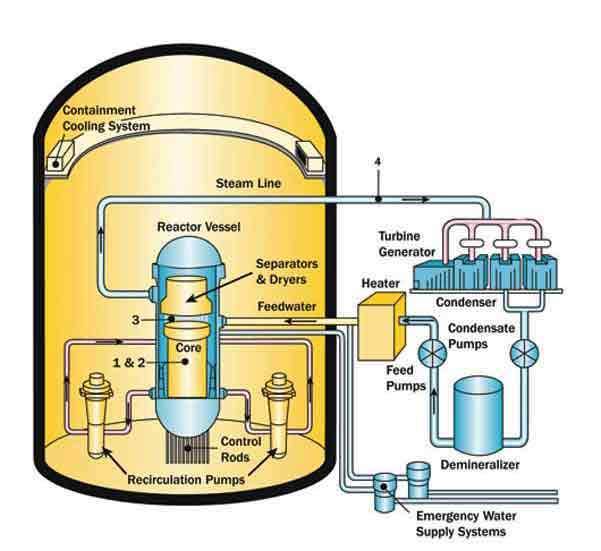
\includegraphics[width=\textwidth]{NRC-BWR.jpg}
 		    \caption{}
 		    \label{subfig:BWR}
 		\end{subfigure}
 		
		\begin{subfigure}[b]{0.65\textwidth}
 		    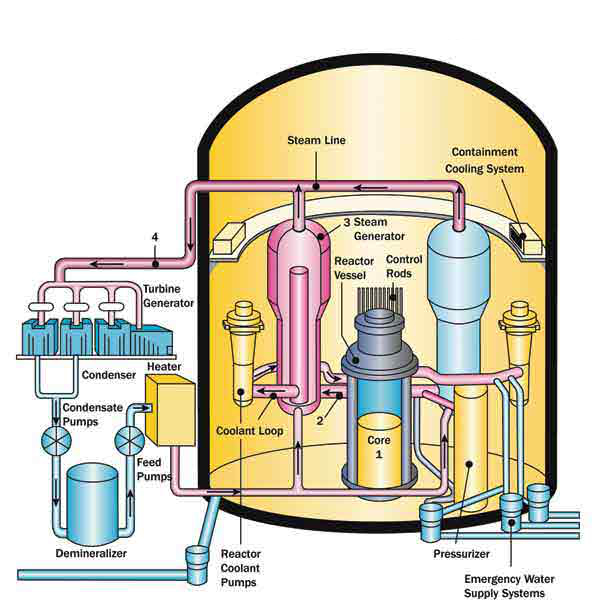
\includegraphics[width=\textwidth]{NRC-PWR.jpg}
 		    \caption{}
 		    \label{subfig:PWR}
 		\end{subfigure}
		\caption[Représentation schématique des technologies:
        a) réacteur à eau bouillante,
        b) réacteur à eau préssurisée.]
        {Représentation schématique des technologies:
        a) réacteur à eau bouillante,
        b) réacteur à eau préssurisée \citep{USNRC2013}.} 
 		\label{fig:Assembly_Control_Blades} 
 	\end{figure}
     \newpage


    

	
    \begin{table}[H]
        \begin{small}
        \centering
        \begin{tabular}{p{0.35\textwidth}p{0.28\textwidth}p{0.28\textwidth}}
        \toprule
        \textbf{Paramètres} & \textbf{REP} & \textbf{REB} \\ \midrule
        Fluide caloporteur & Eau pressurisée & Eau bouillante \\ \hline
        Matériaux des assemblages & Zy-4, Zirlo, Duplex, M5 & Zy-2, Zy-4 \\
                                    & Inconel, SS & Inconel, SS \\ \hline
        Flux de neutrons rapides ($\rm cm^{-2} \, s^{-1}$) &	\num{6}--\num{9e13} &	\num{4}--\num{7e13} \\ \hline
        Température (\si{\degreeCelsius}) & & \\
        Entrée & 279--294 & 272--278 \\
        Sortie & 313--350 & 280--300 \\ \hline
        Pression (bar) & 155--158 & 70--80 \\ \hline
        Vitesse du fluide caloporteur (\si{\meter\per\second}) & 3--6 & 2--5 \\ \hline
        Chimie du fluide caloporteur & & \\
        Oxygène  (\si{\ppb}) & <0.05 & 200--400 \\
        Hydrogène (\si{\ppm}) & 2--4 & 0.02 \\
        Acide borique (\si{\ppm}) & 0--2200 & -- \\
        LiOH (\si{\ppm}) & 0.5--3.5 & -- \\
        \bottomrule
        \end{tabular}
        \caption[Comparaison des paramètres de fonctionnement des technologies REB et REP.]%
        {Comparaison des paramètres de fonctionnement des technologies REB et REP \citep{Adamson2002}.}
        \label{tab:operating_parameters_reactors}
        \end{small}
    \end{table}

%%%%%%%%%%%%%%%%%%%%%%%%%%%%%%%%%%%%%%%%%%%%%%%%%%%%%%%%%%%%%%%%%%%%%%%%%%%%%%%%%%%%%
%%%%%%%%%%%%%%%%%%%%%%%%%%%%%%%%%%%%%%%%%%%%%%%%%%%%%%%%%%%%%%%%%%%%%%%%%%%%%%%%%%%%%
\section{Assemblage de combustible dans un REB}\label{sec:BWR_fuel_assembly}

    Les pastilles d’uranium sont empilées dans un crayon fermé hermétiquement qui
    les isole du fluide caloporteur comme illustré sur la figure \ref{fig:fuel_rod}.
    L’alliage de zirconium Zircaloy-2 est le matériau utilisé pour la fabrication
    des gaines de confinement.

    

    Ces crayons sont regroupés pour former un assemblage combustible dans lequel ils
    sont arrangés en réseau à maille carrée dans une structure assurant notamment
    leur maintien mécanique. Cet arrangement géométrique permet la circulation de
    l’eau entre les crayons et donc la dissipation de la chaleur
    engendrée dans le coeur du réacteur. L’assemblage de combustible est arrangé
    différemment par rapport à un REP à cause des variations de densité du fluide
    caloporteur. Les crayons sont regroupés dans des boîtiers carrés placés aux
    quatre coins de la croix de contrôle comme illustré sur la figure
    \ref{fig:Assembly_Control_Blades}.

    Les grilles de maintien permettent d’assurer la cohésion des crayons.
    Les matériaux généralement utilisés pour la fabrication des grilles de maintien sont des alliages de nickel 718 et
    X750.
    La croix de contrôle, généralement faite en acier
    inoxydable 316L, peut coulisser le long des assemblages de combustible afin
    d’assurer le contrôle de la fission de l’uranium en absorbant les neutrons. 

    Ces deux éléments, grilles de maintien et croix de contrôle, sont
    susceptibles d'induire le phénomène de Shadow Corrosion sur la gaine de confinement en
    Zircaloy-2. 
    Les paragraphes \ref{subsec:Zirconium} à \ref{subsubsec:Zircone} qui suivent donnent quelques informations sur les
    matériaux de gaine et l'oxyde qui se développe à leur surface.

    \newpage
    \begin{figure}[H] 
 		\centering 
 		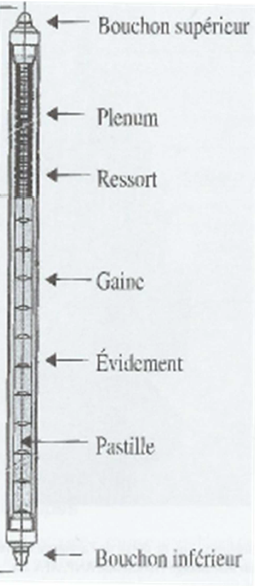
\includegraphics[height=0.40\textheight]{Buttin_2011-Fig1-1.png} 
 		\caption[Représentation schématique d'une gaine de confinement du combustible.]
        {Représentation schématique d'une gaine de confinement du combustible\citep{Coppolani2004}.} 
 		\label{fig:fuel_rod} 
 	\end{figure}

    \begin{figure}[H] 
 		\centering 
 		\begin{subfigure}[b]{0.45\textwidth}
 		    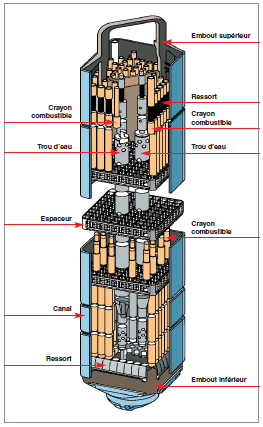
\includegraphics[width=\textwidth]{Pradel_2008-Fig91.png}
 		    \caption{}
 		    \label{subfig:BWR_fuel_assembly}
 		\end{subfigure}
 		\quad \quad \quad
		\begin{subfigure}[b]{0.45\textwidth}
 		    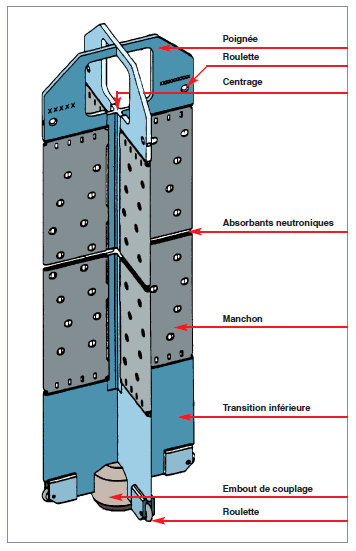
\includegraphics[width=\textwidth]{Pradel_2008-Fig92.png}
 		    \caption{}
 		    \label{subfig:COntrol_Blades}
 		\end{subfigure}
		\caption[Le combustible dans un réacteur à eau bouillante:
        a) assemblage de combustible,
        b) croix de contrôle.]{Le combustible dans un réacteur à eau bouillante:
        a) assemblage de combustible,
        b) croix de contrôle \citep{Pradel2008}.} 
 		\label{fig:Assembly_Control_Blades} 
 	\end{figure}
    \newpage

    
    
	 	
    \subsection{Zirconium pur}\label{subsec:Zirconium}

    Le zirconium répond au cahier des charges des gaines de confinement. En effet,
    ses propriétés physico-chimiques lui confèrent une bonne transparence aux
    neutrons, une bonne conductivité thermique, une bonne résistance mécanique, même
    à haute température et une bonne étanchéité entre les pastilles d'uranium et le fluide caloporteur.
    Les principales propriétés physiques du zirconium sont résumées dans le tableau \ref{tab:physical_properties_zirconium}. 

    Il faut noter que la principale raison du choix du zirconium réside dans sa
    faible section de capture des neutrons qui est environ 30 fois inférieure à celle
    des aciers inoxydables. Les caractéristiques
    métallurgiques du zirconium sont liées à sa forte réactivité avec l’oxygène, aux
    différentes interactions chimiques avec les éléments d’alliages (solubilité
    totale ou formation de phases intermétalliques) et à sa structure anisotropique
    hexagonale compacte qui conduit au développement d'un matériau texturé après
    traitement thermomécanique. 


    \begin{table}[H]
        \begin{small}
            \centering
            \begin{tabular}{p{0.45\textwidth} p{0.13\textwidth} p{0.13\textwidth} p{0.13\textwidth}}
                \toprule
                 & \textbf{Moyenne} & \textbf{Direction [1120]} & \textbf{Direction [0001]} \\ \midrule
                Masse volumique (\si{\kilogram\per\cubic\meter}) & 6500 & -- & -- \\ \hline
                Dilatation thermique (\si{\per\kelvin}) & \num{6.7e-7} & \num{6.7e-6} & \num{10.4e-6} \\\hline
                Module de Young (GPa) & -- & 99 & 125 \\\hline
                Paramètre de réseau (\si{\nano\meter}) & -- & a=0.323 & c=0.515 \\\hline
                Conductivité thermique (\si{\watt\per\meter\per\kelvin})  & 22 & -- & -- \\\hline
                Chaleur spécifique (\si{\joule\per\kilogram\per\kelvin}) & 276 & -- & -- \\\hline
                Section de capture de neutron \newline (1~barn= $10^{-28}m^2$) & 0.185 & -- & -- \\
                \bottomrule
            \end{tabular}
            \caption[Propriétés physique du zirconium.]{Propriétés physiques du zirconium \citep{IAEA1998}.}
            \label{tab:physical_properties_zirconium}
        \end{small}
    \end{table}

    
    

    A température ambiante, la forme allotropique stable du zirconium est hexagonale
    compacte avec un ratio c/a égale à 1.593. Les paramètres du réseau cristallin a
    et c ont pour valeur \SI{0.323}{\nano\meter} et  \SI{0.515}{\nano\meter},
    respectivement \citep{Douglass1971}. Les différences de dilatation thermique
    entre les directions a et c impliquent que le ratio c/a tend vers le ratio idéal (1.633)
    à plus haute température. Le zirconium fond à
    \SI{1860}{\degreeCelsius}, et par conséquent, il peut être considéré comme un
    métal modérément réfractaire.

    Lors des refroidissements après traitement thermique, le zirconium subit une transformation allotropique de la structure
    cubique centrée $\beta$ vers la structure hexagonale compacte $\alpha$.
    En fonction de la vitesse de refroidissement, la transformation peut être
    martensitique ou bainitique. L’épitaxie des plaquettes de la phase $\alpha$ sur
    les anciens grains de la phase $\beta$ conduit à une microstructure avec un
    ensemble d’orientations cristallographiques identiques à celles de la phase
    $\beta$ formant ainsi une microstructure à plaques parallèles. 

    

    \subsection{Alliage Zircaloy-2}\label{subsec:Zircaloy-2}

    La solubilité relative des différents éléments d’alliage dans les phases
    $\alpha$ et $\beta$ est un critère de premier ordre pour le choix des quantités à dissoudre
    et des traitements thermiques à effectuer. Le tableau
    \ref{tab:zircaloy_chemical_composition} liste les spécifications ASTM en termes de
    composition chimique des alliages Zircaloy-2. Les différentes nuances ont été développées 
    pour s'adapter aux différents REB mis en service.

    

    L’étain stabilise la phase $\alpha$ dans laquelle il se retrouve en solution
    solide. Il fut, originellement, ajouté afin de contrer les effets néfastes de
    l’azote en termes de résistance à la corrosion. Avec les améliorations des
    procédés de fabrication, il est maintenant possible de diminuer la teneur en
    étain, dont on notera qu'il a également un impact sur les propriétés mécaniques. 

    Le fer, le chrome et le nickel ont une solubilité très limitée dans la phase
    $\alpha$ et se retrouvent sous formes de précipités dans la matrice métallique.
    Deux types de précipités se forment: les phases de laves $\rm Zr(Fe,Cr)_2$ et
    les phases de Zintl $\rm Zr_2(Fe,Ni)$. La présence et la taille de ces
    précipités sont deux paramètres importants pour la résistance à la corrosion
    \citep{Barberis2005}. 

    \begin{table}[H]
        \begin{small}
        \centering
        \begin{tabular}{p{0.2\textwidth}%
                        p{0.12\textwidth}%
                        p{0.12\textwidth}%
                        p{0.12\textwidth}%
                        p{0.12\textwidth}%
                        p{0.12\textwidth}}
        \toprule
        \textbf{ASTM Ref.} & \textbf{Sn (\%wt.)} & \textbf{Fe (\%wt.)} & \textbf{Cr (\%wt.)} & \textbf{Ni (\%wt.)} & \textbf{O (ppm)} \\ \midrule
        R 60802 Zircaloy-2 & 1.2--1.7 & 0.07--0.20 & 0.05--0.15 & 0.03--0.08 & 1000--1400\\
        \bottomrule
        \end{tabular}
        \caption[Composition chimique (ASTM) de l'alliage Zircaloy-2.]{Composition chimique de l'alliage Zircaloy-2 \citep{IAEA1998}.}
        \label{tab:zircaloy_chemical_composition}
        \end{small}
    \end{table}



    \subsection{Zircone}\label{subsubsec:Zircone}

    Lors de l’exposition des gaines de confinement dans l’environnement d’un REB en fonctionnement,
    une couche d'oxyde de zirconium ($\rm ZrO_2$) se développe rapidement en
    surface \citep{Cox2011}. 
    La zircone existe sous trois variétés polymorphiques:
    \emph{monoclinique}, \emph{quadratique} et \emph{cubique}.
    Les mailles élémentaires sont
    illustrées sur la figure \ref{fig:Zirconia_allotropic_forms} alors que les domaines d’existence ainsi que les
    paramètres de maille sont résumés dans le tableau \ref{tab:zirconia_allotropic_forms}.
   

    Dans les conditions de pression et de température d’un REB, la phase stable de
    la zircone est donc la forme monoclinique. La différence de volume entre la
    maille de zircone monoclinique et la maille hexagonale compacte du zirconium métallique
    sous-jacent conduit à un ratio de Pilling-Bedworth de 1.56 dont la conséquence est
    la présence de contraintes de compression à l’interface métal/oxyde. Ces contraintes
    mécaniques ainsi que l'irradiation ou la présence des précipités peuvent favoriser
    la stabilisation de la phase quadratique à l'interface métal/oxyde \citep{IAEA1998}. 

    \begin{figure}[H] 
 		\centering 
 		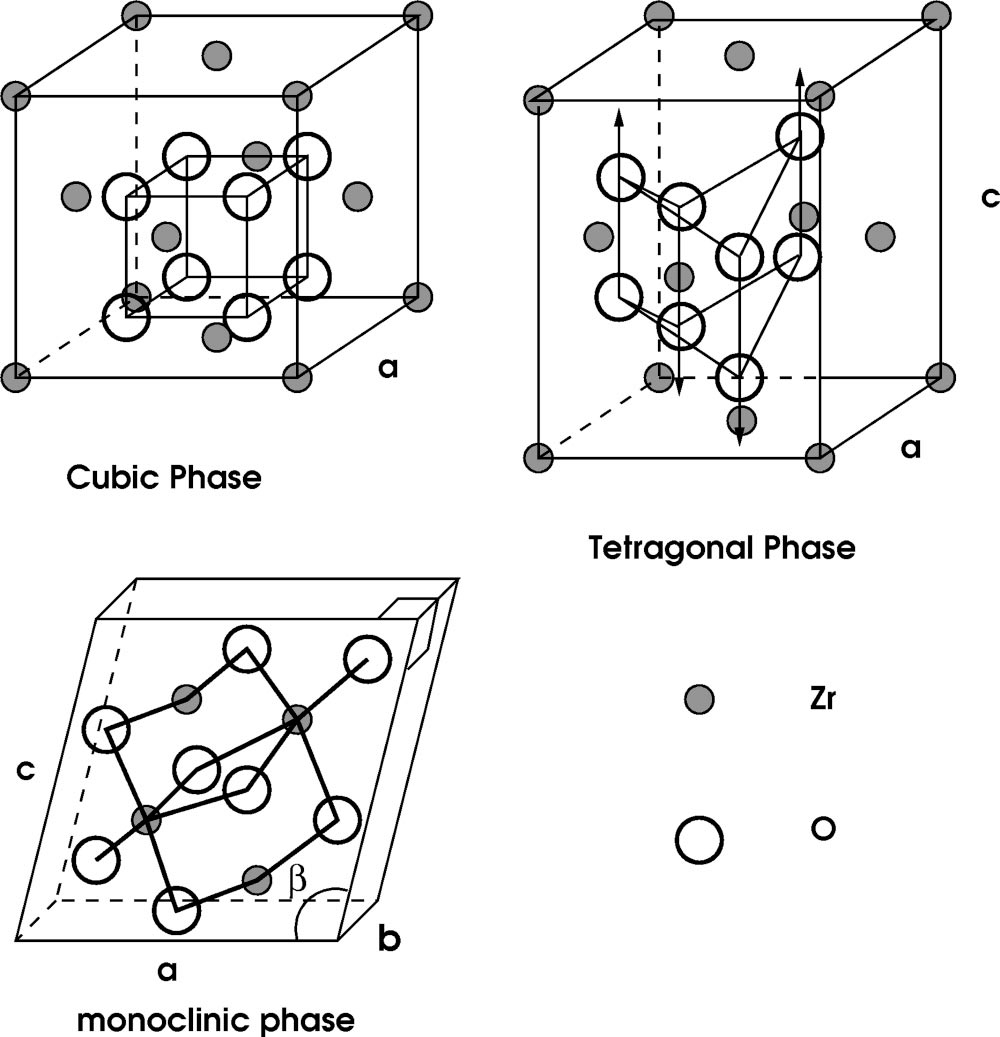
\includegraphics[width=0.59\textwidth]{Zhao_2002-Fig1.png} 
 		\caption[Les différentes phase de la zircone.]
        {Les différentes phases de la zircone \citep{Zhao2002}.
        Pour la phase quadratique (tetragonal en anglais), les flèches indiquent les distorsions du réseau par rapport à la phase cubique.} 
 		\label{fig:Zirconia_allotropic_forms} 
 	\end{figure}


    \begin{table}[H]
        \begin{small}
        \centering
        \begin{tabular}{p{0.30\textwidth} p{0.25\textwidth} p{0.35\textwidth}}
        \toprule
        \textbf{Variété polymorphique}    & \textbf{Température (°C)} & \textbf{Paramètre de maille (nm)} \\
        \midrule
        Monoclinique ($\rm m-ZrO_2$)      & T<1127    & a=0.510; b=0.516; c=0.527; $\beta$=99\si{\degree}21\si{\arcminute}      \\
        Quadratique ($\rm t-ZrO_2$)      & 1127<T<2297    & a=0.502; b=0.509 \\
        Cubique ($\rm c-ZrO_2$)      & 2297<T<2707    & a=0.503 \\
        \bottomrule
        \end{tabular}
        \caption[Domaine d'existence et paramètre de maille des variétés polymorphiques de la zircone.]
        {Domaine d'existence et paramètre de maille des variétés polymorphiques de la zircone \citep{Zhao2002}.}
        \label{tab:zirconia_allotropic_forms}
        \end{small}
	\end{table}

    Les propriétés d'isolant électrique de la zircone sont liées à la valeur de bande
    interdite élevée soit 5~eV \citep{Benaboud2007, Morrison1980}, mais sa résistivité varie sensiblement en présence
    d'impuretés.
    On considère généralement que la conductivité électrique et la conductivité ionique des couches d'oxydation du
    Zircaloy-2 sont séparées c'est-à-dire que la conductivité électrique est liées aux précipités alors
    que la conductivité ionique est liée aux défauts de la couche \citep{IAEA1998}. 

    Dans la suite du manuscrit, sauf indication contraire, les couches d'oxydation des alliages de zirconium seront
    dénommés \emph{couches de zircone}. 
    

	
\newpage
%%%%%%%%%%%%%%%%%%%%%%%%%%%%%%%%%%%%%%%%%%%%%%%%%%%%%%%%%%%%%%%%%%%%%%%%%%%%%%%%%%%%%
%%%%%%%%%%%%%%%%%%%%%%%%%%%%%%%%%%%%%%%%%%%%%%%%%%%%%%%%%%%%%%%%%%%%%%%%%%%%%%%%%%%%%
\section{Oxydation des alliages de zirconium}\label{sec:oxidation_zirconium}

    Dans un premier temps, la quantification de l'oxydation des alliages de zirconium est abordée en présentant la
    conversion des prises de masse en épaisseur de couche de zircone équivalente et en densité de courant d'oxydation équivalente. 
    Ensuite, l'analyse de l'oxydation hors irradiation
    permet de présenter les points clés en termes de cinétique, de porteurs de charge dans la couche de zircone et de
    processus limitant, complétée par une analyse de l'oxydation sous irradiation.

    \subsection{Quantifications de l'oxydation}\label{subsec:oxidation_introduction}


    Le diagramme de phase du système Zr/O est illustré en figure \ref{fig:ZrO_thermodynamics}. Il
    indique que tout l'oxygène n'est pas sous forme d'oxyde. Une partie de l'oxygène est dissoute
    dans la matrice $\alpha$ de zirconium. La proportion d'oxygène dissous est encore mal connue et elle dépend de
    l'équilibre entre les cinétiques d'oxydation et de dissolution. Tout changement de cinétique
    d'oxydation aura un impact sur l'extension spatiale de la zone de diffusion de l'oxygène dissous.
    Cependant, la quantité d'oxygène dissous est faible au regard de celle engagée dans les oxydes formés aux
    températures de fonctionnement d'un réacteur à eau bouillante.

    \begin{figure}[H]
    \centering
    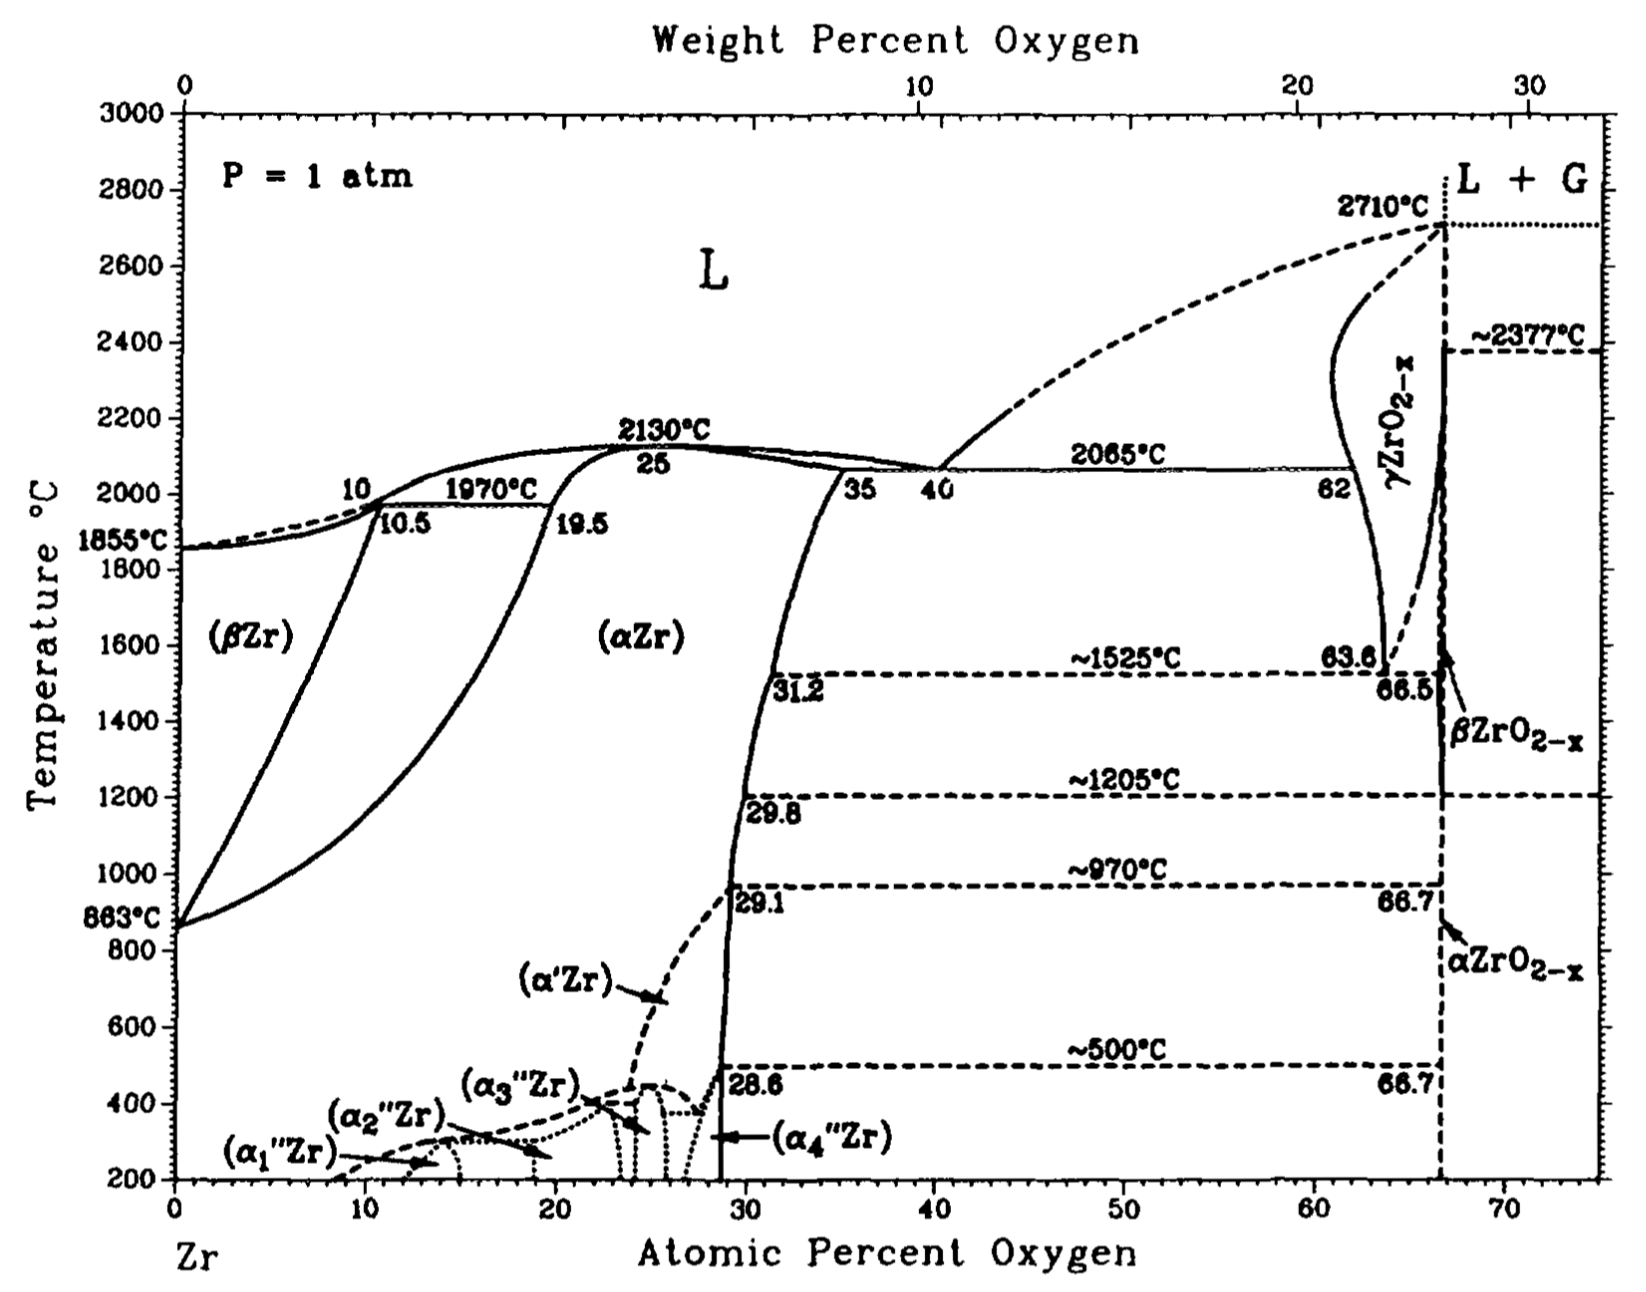
\includegraphics[width=0.85\textwidth]{IAEA_1998_Fig2_1a.png}
    \caption[Diagramme de phase du système ZrO/O]{Diagramme de phase du système Zr/O \citep{IAEA1998}.}
    \label{fig:ZrO_thermodynamics}
    \end{figure}

    Les cinétiques de croissance de l'oxyde sont donc généralement obtenues à partir des cinétiques expérimentales de prise de masse. L'hypothèse
    sous-jacente est que l'intégralité de la couche de zircone formée reste sur l'échantillon et que cette dernière est
    homogène sur l'ensemble de la surface exposée. Les cinétiques de prise de 
    masse sont converties en épaisseurs d'oxyde en utilisant la masse volumique théorique de $ZrO_2$ soit 
    \SI{5.68}{\gram\per\cubic\centi\meter} \citep{Lide2003}.
    %ce qui est une approximation car une partie des précipités
    %sont oxydés et bien d'avantage en raison de l'oxygène qui est dissout dans le métal sous-jacent.
    Le rapport de conversion de
    \SI{15}{\milli\gram\per\square\deci\meter} par micron d'épaisseur d'oxyde obtenue avec cette valeur de masse volumique
    reste une approximation, mais une utilisation standardisée permet  une première comparaison des
    cinétiques d'oxydation de différents alliages.

    Etant donné que le présent travail de thèse comporte une étude électrochimique de l'oxydation des alliages de zirconium, il est
    nécessaire de pouvoir convertir les cinétiques de croissance d'oxyde en densités de courant d'oxydation équivalentes.
    Sur la base des hypothèses formulées pour la conversion des prises de masse en épaisseur équivalente, il est
    possible de convertir une épaisseur d'oxyde en densité de courant
    d'oxydation en effectuant une approximation au premier ordre selon la loi de Faraday \citep{Bard2001}. Cette
    conversion est intéressante car la densité de courant, $j$, est une image de la vitesse d'oxydation.
    A partir des demi-réactions anodiques et cathodiques associées \citep{Adamson2007} à la corrosion du zirconium 
    (éq. \ref{eq:anodic_half_reaction} et \ref{eq:cathodic_half_reaction}),
    il est possible d'exprimer la densité de courant, j, en fonction de l'épaisseur de la
    couche de zircone, $d_{ZrO_2}$, par l'équation \ref{eq:th_to_j}. 



    \begin{equation}
        \text{Interface interne: }Zr_{metal} \rightarrow Zr_{Zr}^x + 4e^{-} + 2V_O^{\bullet \bullet}
        \label{eq:anodic_half_reaction}
    \end{equation}

    \begin{equation}
        \text{Interface externe: }2V_O^{\bullet \bullet} + 2 H_2O + 4e^{-}  \rightarrow 2O_O^x + 2H_2 \\
    \label{eq:cathodic_half_reaction}
    \end{equation}


    \begin{equation}
    \begin{split}
        \mathit{j} &= \frac{4F\rho _{ZrO_2}}{M_{ZrO_2}}\frac{d}{d\mathit{t}} \mathit{d_{\mathrm{ZrO_2}}}\\
        \mathit{j}[\si{\micro\ampere\per\square\centi\meter}] &\approx \num{1.78e6}
        \frac{d}{d\mathit{t}} \mathit{d_{\mathrm{ZrO_2}}} \frac{[\si{\micro\meter}]}{[\si{\second}]}
    \end{split}    
    \label{eq:th_to_j}
    \end{equation}


    \subsection{Oxydation hors irradiation}\label{subsec:no_irradiation}
    
    \subsubsection{Cinétiques d'oxydation}\label{subsubsec:oxidation_kinetics}
    
    Les expositions de Zircaloy-2 en milieu aqueux à différentes températures montrent que la cinétique d'oxydation du Zircaloy-2 est
    relativement lente en autoclave comme illustré sur la figure \ref{fig:Zy2_Kinetics_vs_T}, où les courbes à
    \SI{275}{\degreeCelsius} et \SI{300}{\degreeCelsius} sont représentatives des températures d'entrée et de sortie d'un
    réacteur à eau bouillante. Après un an d'oxydation en
    autoclave, la couche de zircone présente une épaisseur de seulement quelques microns. 

    La figure \ref{fig:Zy2_Kinetics_vs_T_J} montre en fonction du temps la densité de courant anodique obtenue par
    numérisation des données de
    la figure \ref{fig:Zy2_Kinetics_vs_T} et application de l'équation \ref{eq:th_to_j}. Dans les premiers instants de
    l'oxydation, la densité de courant est comprise entre 2 et 5 \si{\micro\ampere\per\square\centi\meter}, elle passe 
    rapidement sous le seuil de \SI{1}{\micro\ampere\per\square\centi\meter}, ainsi
    après 10 jours d'oxydation, la densité de courant vaut environ \SI{0.5}{\micro\ampere\per\square\centi\meter}, et après 50 jours,
    elle devient inférieure à \SI{0.1}{\micro\ampere\per\square\centi\meter} pour atteindre
    environ \SI{0.05}{\micro\ampere\per\square\centi\meter} après un an d'oxydation. Cette première analyse est certes
    simpliste mais elle fournit des ordres de grandeur pour les valeurs de densité de courant typiques qui seront
    mesurables en autoclave hors irradiation.

    \begin{figure}[H]
        \centering
        \begin{subfigure}[b]{0.65\textwidth}
            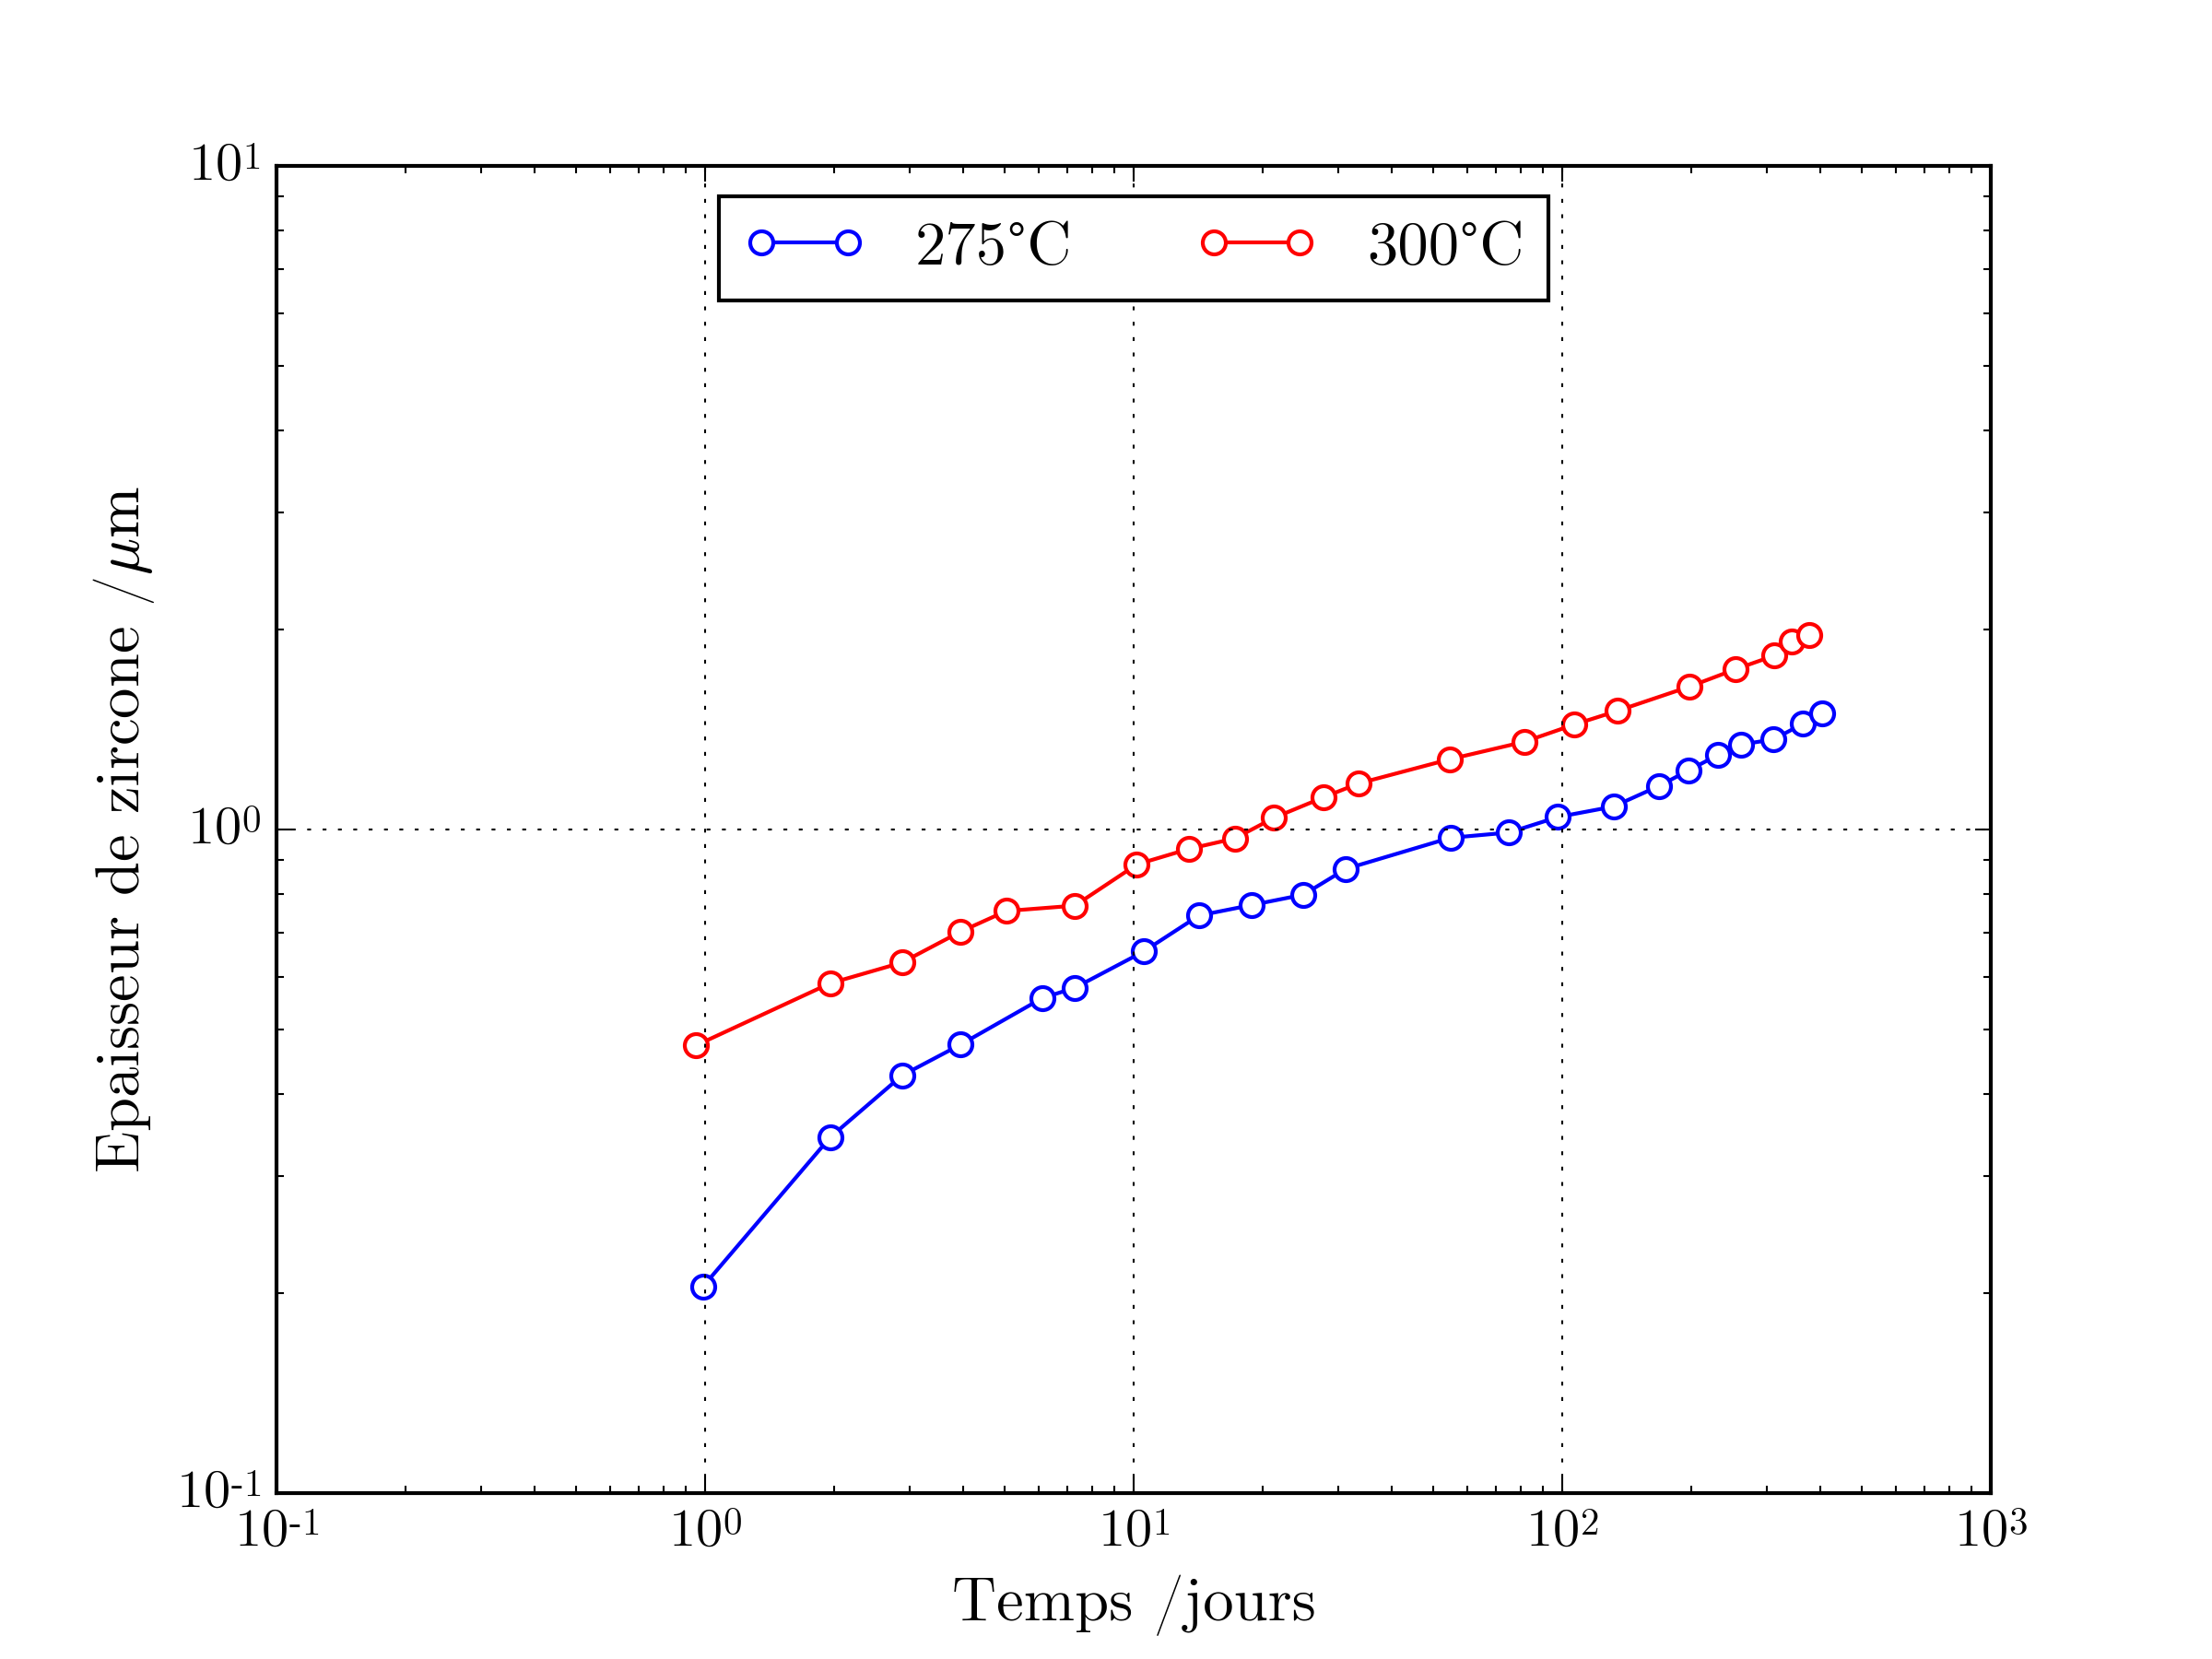
\includegraphics[width=\textwidth]{Cox_1968-Fig2-th.png}
            \caption{}
            \label{fig:Zy2_Kinetics_vs_T}
        \end{subfigure}
        \begin{subfigure}[b]{0.65\textwidth}
            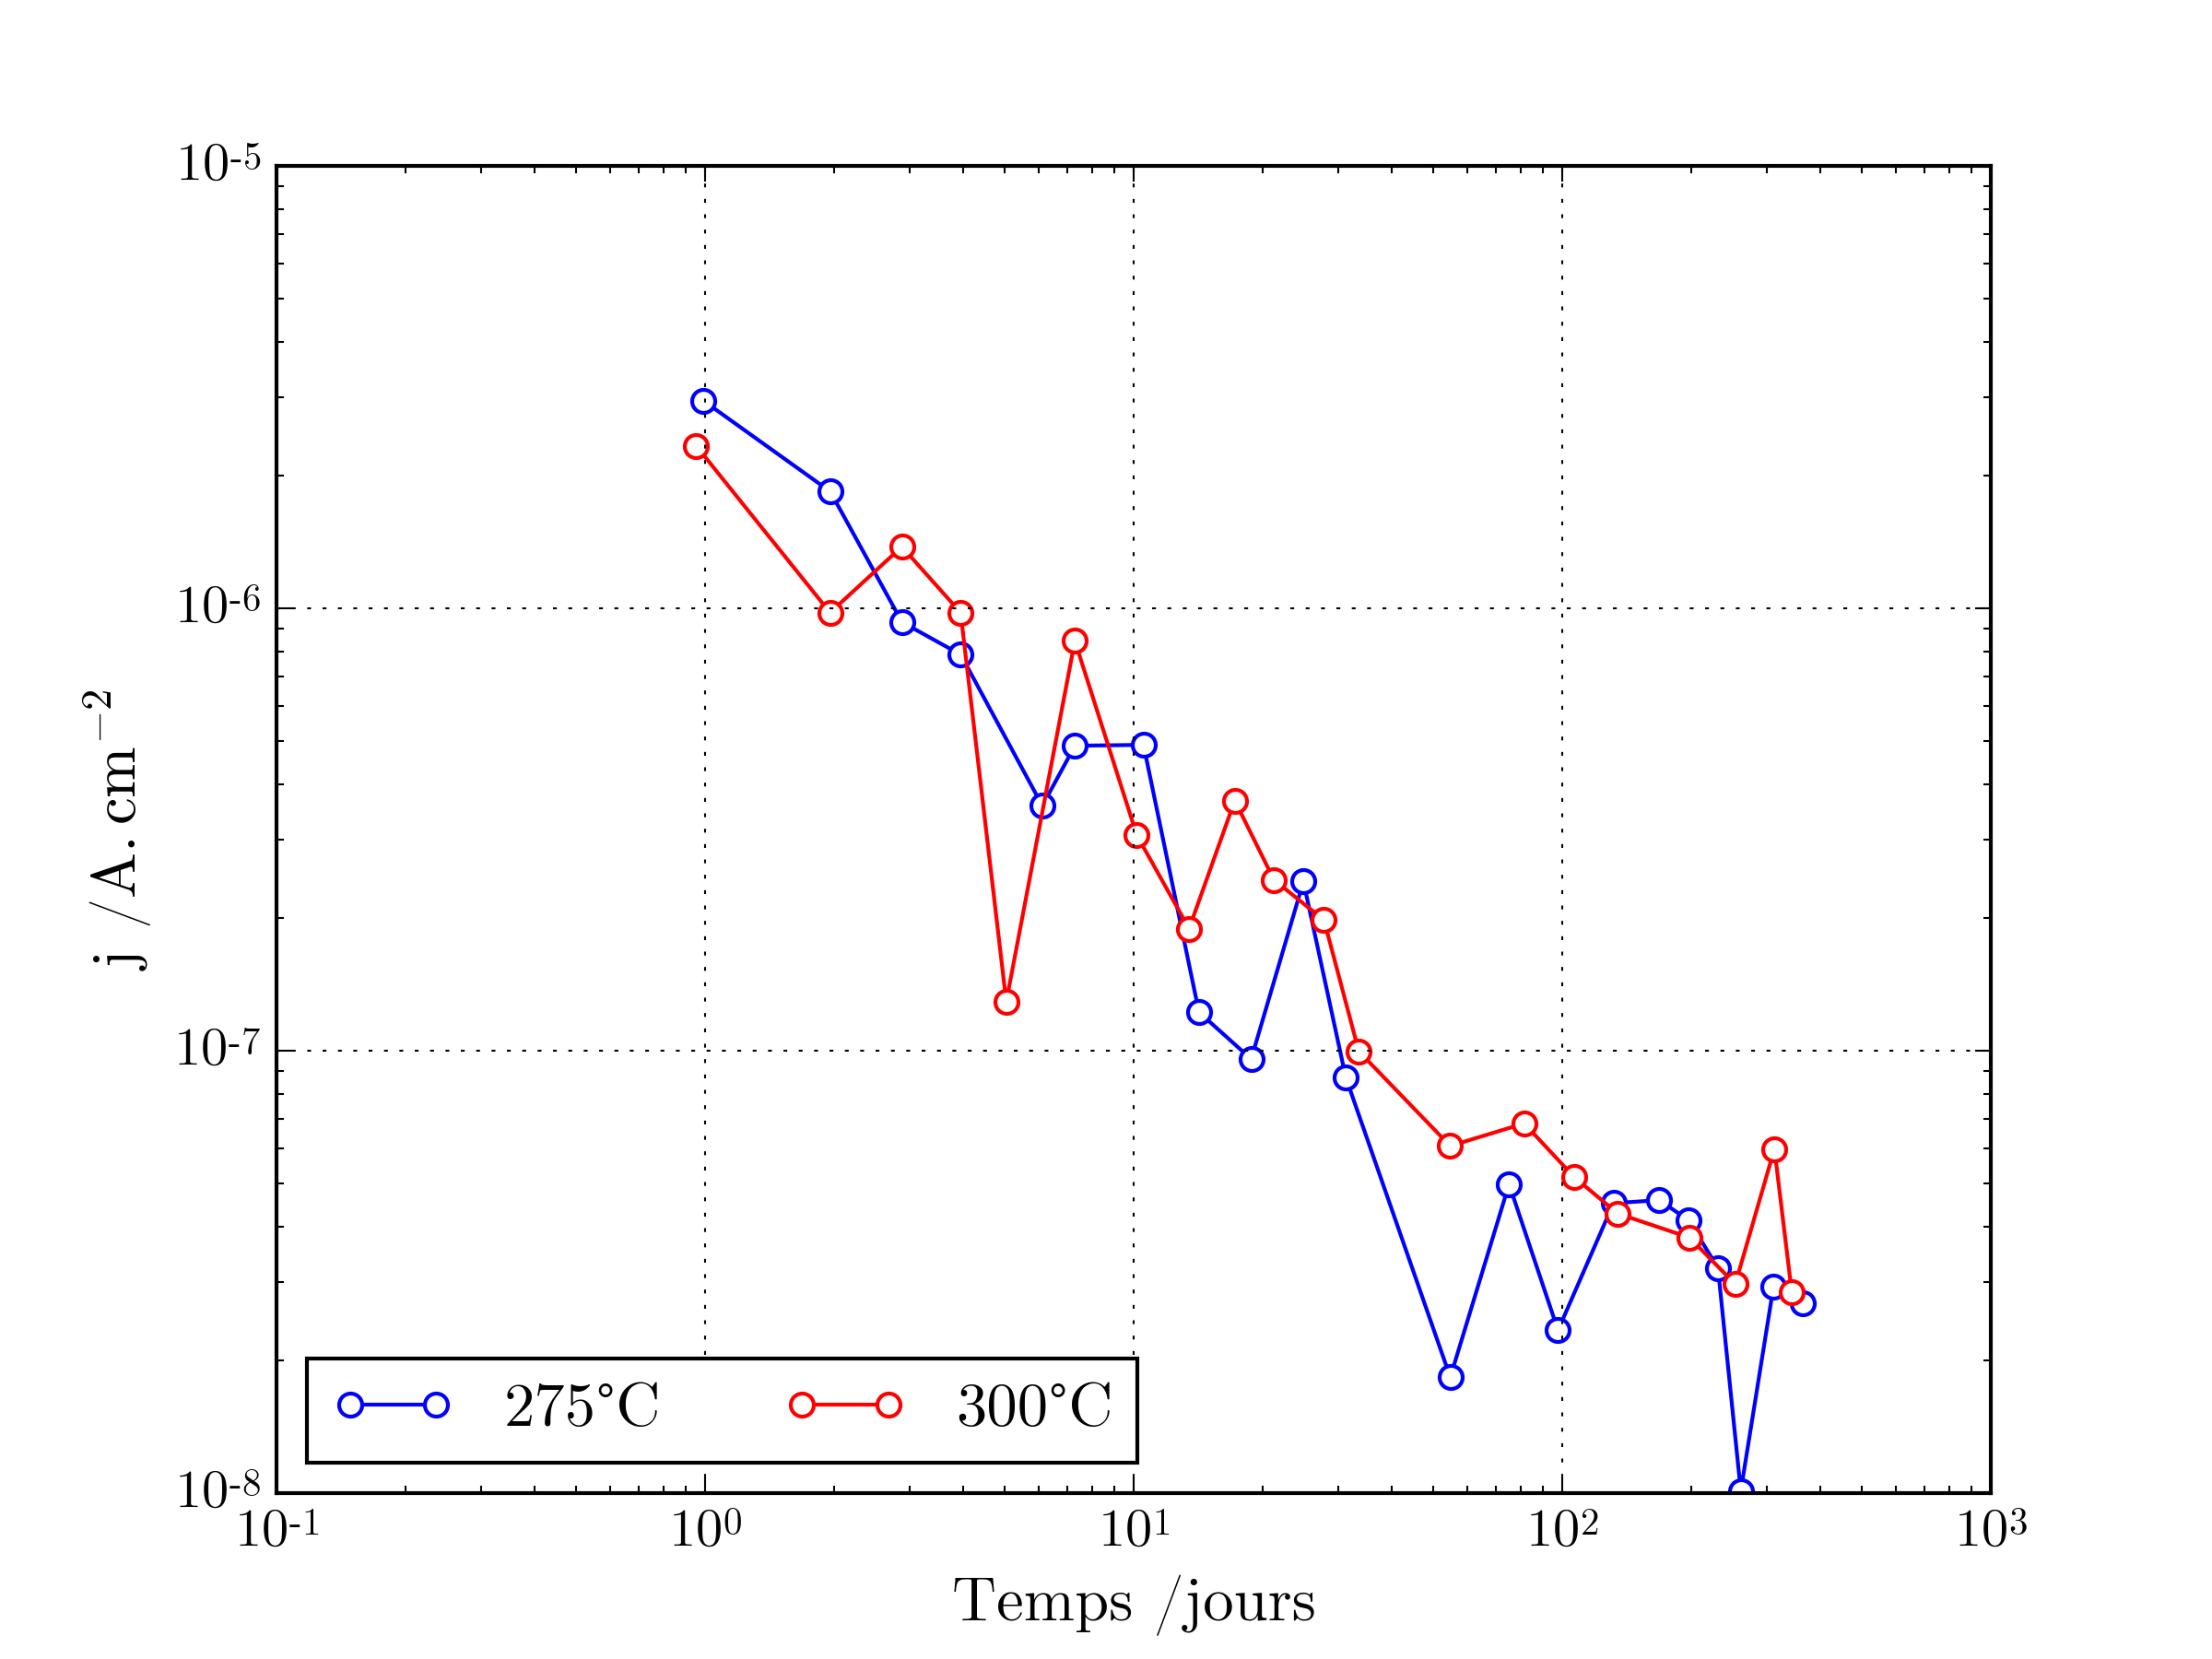
\includegraphics[width=\textwidth]{Cox_1968-Fig2-J.png}
            \caption{}
            \label{fig:Zy2_Kinetics_vs_T_J}
        \end{subfigure}
        \caption[Cinétique d'oxydation de l'alliage Zircaloy-2 en eau déminéralisée et désaérée à différentes
        températures.]{Cinétique d'oxydation de l'alliage Zircaloy-2 en eau déminéralisée et désaérée à différentes
        températures:
        a) évolution de la croissance de la couche de zircone \citep{Cox1968-1}, b) évolution de la densité de courant équivalente.}
        \label{fig:ch1_Zy2_Kinetics_th_J}
    \end{figure}


    La cinétique d'oxydation comporte deux régimes distincts (dits \emph{pré-transition} et \emph{post-transition}) séparés par
    une phase de \emph{transition}, comme illustré en figure \ref{fig:Zy2_Kinetics_Regimes}. 
    %La couche de zircone formée lors du 
    %régime de pré-transition est dense alors que la couche formée lors du régime de post-transition est poreuse
    %\citep{IAEA1998}. 
    La couche de zircone formée lors du régime de pré-transition est plus dense que la couche formée lors du régime de
    post-transition \citep{IAEA1998}.
    Généralement, la phase de \emph{transition} débute lorsque la couche de zircone atteint
    environ \SI{2}{\micro\meter}.

    Lors du régime de pré-transition, le profil cinétique d'oxydation est sub-parabolique, et non parabolique
    comme attendu pour une diffusion volumique de l’oxygène dans l’approximation de \citet{Wagner1933}.
    \citet{Dali2007} résume l'ensemble des lois cinétiques proposées pour le régime pré-transitoire avec 
    des descriptions mécanistiques particulières, qui ont été testées par
    ajustement aux données expérimentales. Par exemple, \citet{Smeltzer1961} proposent une loi cinétique basée sur la diffusion de
    l'oxygène aux joints de grain alors que \citet{Eloff1991} proposent un modèle où la cinétique est contrôlée par un
    champ électrique dans la couche de zircone en s'appuyant sur la théorie de \citet{Fromhold1980}. Par ailleurs,
    \citet{Cox1968-1} a montré par des
    expériences de marquage isotopique que la diffusion aux joints grains est nettement plus rapide que celle en volume.
    Il estime par conséquent que la vitesse est contrôlée par le transport de l’oxygène aux joints de grains. Comme la
    taille des grains augmente au cours de l’oxydation, cette croissance se traduit,
    d’après l’auteur, par une réduction sensible de la surface efficace de diffusion aux joints de grains et donc par
    une diminution de la vitesse par rapport à celle déduite de la loi parabolique.


            
    
    \begin{figure}[H]
        \centering
        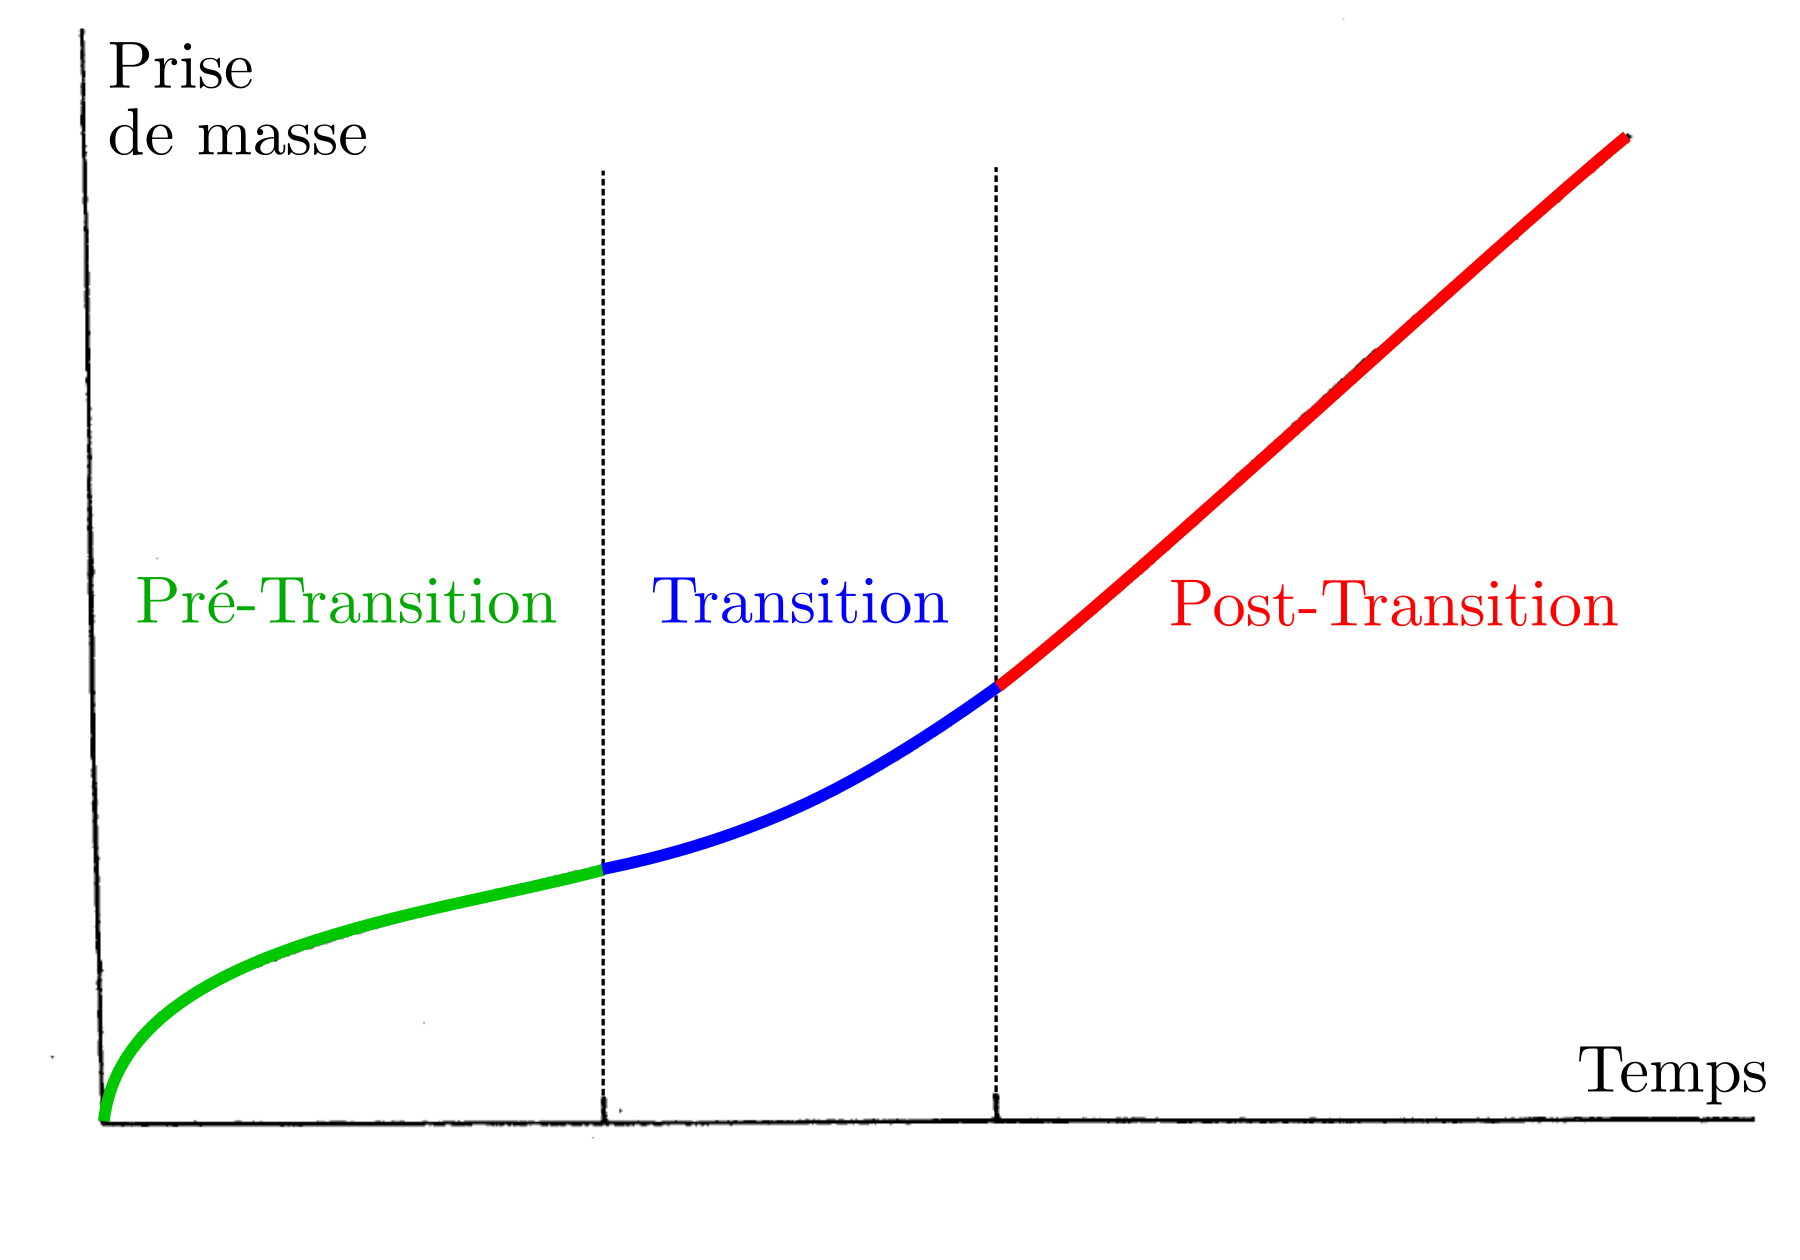
\includegraphics[width=0.65\textwidth]{Kinetics_Periods.png}
        \caption[Illustration des deux régimes de cinétique d'oxydation. Le deux régimes sont séparés par une phase de
        transition.]{Illustration des deux régimes de cinétique d'oxydation. Le deux régimes sont séparés par une phase de
        transition \citep{Cox2005}.}
        \label{fig:Zy2_Kinetics_Regimes}
    \end{figure}


    
    Comme déjà mentionné précédemment, la phase de transition apparaît lorsque l'épaisseur de la couche de zircone atteint
    environ \SI{2}{\micro\meter} \citep{IAEA1998}. Elle se traduit par l'apparition d'un changement de cinétique
    d'oxydation. La relaxation des contraintes dans la couche de zircone serait la première explication de la transition
    cinétique, en raison d'une
    fissuration (parallèle à l'interface) de la couche de zircone liée à des différences de contraintes dans l'épaisseur de l'oxyde.
    %La
    %différence de volume molaire entre le métal et la couche de zircone crée des contraintes de compression à l'interface
    %métal/oxyde alors que le rayon de courbure de la gaine crée des contraintes de traction à la surface externe de la couche de zircone,
    %favorables à l'initiation de fissures perpendiculaires à l'interface.
    %Cependant, les fissures perpendiculaires ne devraient pas se propager plus loin que l'axe des contraintes nulles laissant ainsi une
    %couche interne intacte. 
    La présence de fissures, perpendiculaires à l'interface, pénétrant jusqu'à l'interface métal/oxyde a été évoquée
    mais est encore débattue.
    La transition peut présenter différents mode de développement dans différentes conditions expérimentales
    \citep{Cox1968-1}. 
    Par exemple, en solutions aqueuses entre \SI{300}{\degreeCelsius} et \SI{360}{\degreeCelsius}, la transition peut être très
    soudaine, impliquant une forte augmentation de la cinétique d'oxydation. Pour des températures plus élevées, en présence
    de vapeur d'eau et d'oxygène, la transition est plus douce.
    %Enfin, une transition de type para-linéaire caractérisée par un changement de cinétique d'oxydation
    %constant de la cinétique sub-parabolique vers la cinétique linéaire en passant par la cinétique parabolique sans aucune accélération de la cinétique
    %d'oxydation.  
    
    Le profil cinétique d'oxydation du régime post-transition est, suivant les auteurs, soit un profil
    ressemblant à une succession de régimes de pré-transition dont l’amplitude diminue avec le temps
    \citep{Garcia1999}, soit un profil cinétique linéaire \citep{Vermoyal2002}. La différence entre ces deux profils dépend des
    conditions d’oxydation et des nuances d’alliage considérées.

    

    \subsubsection{Porteurs de charge dans la couche de zircone}\label{subsubsec:charge_carrier}

    En l'abscence de potentiel appliqué à l'échantillon, le courant d'oxydation correspondant à la demi-réaction anodique et le courant de réduction
    correspondant à la demi-réaction cathodique qui sont égaux et de signe opposé. Si cette condition d'électroneutralité n'est pas
    respectée dans les premiers instants de la formation de la couche de zircone, une différence de potentiel apparaît dans
    la couche de zircone entre l'interface métal/oxyde et l'interface oxyde/environnement dont l'effet est d'égaliser ces
    deux courants \citep{Cox1969}. La diffusion cationique (ions $Zr^{4+}$) est quasi inexistante dans la couche de
    zircone et seule
    la diffusion anionique (ions $O^{2-}$) a lieu au niveau des joints de grain possédant une concentration élevée de
    lacunes \citep{Cox1968-1,Brossmann1999}. Le transport dans la couche de zircone est de type lacunaire c'est-à-dire que des
    lacunes sont crées à l'interface métal/oxyde et diffusent vers l'interface oxyde/environnement. 

    Par conséquent, si les ions oxygène sont les seules espèces ioniques mobiles, l'électroneutralité dans la couche
    d'oxyde peut seulement être respectée avec un flux d'électrons dans le sens opposé. Le transport des électrons a
    probablement lieu par saut entre les atomes immobiles de Zr de la couche de zircone. Les phases intermétalliques,
    $Zr(Fe,Cr)_2$ et $Zr_2(Fe,Ni)$ dans la couche de zircone, sont potentiellement des sites de conduction électronique pour les électrons
    \citep{IAEA1998}.
    \citet{Sundell2012} ont récemment montré que le transport des électrons peut être favorisé par la ségrégation de Fe et
    de Ni aux joints de grain de la couche de zircone. Sur la base des ces résultats, la présence des phases intermétalliques peut
    paraître néfaste en termes de résistance à la corrosion. Cependant, la relation entre la présence des phases
    intermétalliques et la résistance à la corrosion n'est pas aussi tranchée. En effet, \citet{Barberis2005} ont 
    montré qu'un zirconium sans les précipités (dans le métal) avait une très faible résistance à la corrosion sous eau, par rapport à
    un zirconium contenant des précipités.  
     

    \citet{Shirvington1970-1} a étudié l'effet sur la conductivité de la couche de zircone des conditions
    oxydantes lors de sa formation. Il propose trois modèles de structure de couche de zircone en surface de phases intermétalliques dans
    l'alliage Zircaloy-2 comme illustré sur la figure \ref{fig:shirvington_oxide_structures}. Les modèles proposés ici sont
    basés sur l'analyse de courbes de polarisation mesurés en milieu sel fondu.

    Le modèle (i) correspond à la situation où le métal est à un potentiel très cathodique. Dans ce cas, les
    éléments plus nobles tels que Fe, Cr et Ni ne s'oxydent pas ou peu, avec pour conséquence la formation d'une couche
    de zircone non dopée. Les oxydes formés en milieu aqueux désaéré sont susceptibles de développer ce genre de
    structure.

    Le modèle (ia) est une structure
    supplémentaire pouvant apparaître dans les premiers instants de l'oxydation dans un environnement favorisant la
    cristallisation de magnétite $Fe_3O_4$ présentant une semi-conduction de type \emph{p}. L'augmentation de conductivité
    électronique peut être liée à l'injection de trou provenant de la bande de valence de la magnétite dont la
    conséquence sur les courbes de polarisation est de faciliter la demi-réaction cathodique

    Le modèle (ii) correspond à la situation où le métal est à un potentiel élevé, soit en raison d'un couplage, soit
    que la différence de potentiel dans la couche de zircone soit faible.
    Les
    éléments Fe, Ni, Cr peuvent alors se dissoudre dans la matrice de zircone et doper cette dernière. La présence d'hématite,
    présentant une semi-conduction de type \emph{n}, en
    surface n'est pas à exclure. Les oxydes formés en milieu aqueux oxygéné peu conducteur sont susceptibles de
    développer ce type de structure. Cependant, les courbes de polarisation mesurées montre un faible impact sur la
    conductivité électronique. L'ensemble de la structure peut être considéré comme un oxyde ayant une semi-conduction
    de type \emph{n}.


    Le modèle (iii) correspond à une situation intermédiaire entre le modèle (ia) et (ii). Ce modèle est envisageable
    lorsque le potentiel du métal se trouve à une valeur intermédiaire en milieu aqueux
    oxygéné. L'élément Fe (éventuellement Cr et Ni) peut se dissoudre dans la matrice de zircone, dopant cette
    dernière comme dans le modèle (ii). La diffusion jusqu'à l'interface externe pour former de la magnétite
    est éventuellement possible (modèle (ia)). Une partie de la magnétite est convertie en hématite. La conductivité
    électronique de la couche de zircone peut être liée à l'injection de trous provenant de la bande de valence de la
    magnétite. Il faut noter qu'un alignement adéquat des bandes de valence et de conduction, selon que les oxydes sont
    en appauvrissement
    ou en accumulation de porteurs de charge majoritaires, ainsi que des largeurs de bande interdite particulières 
    sont nécessaires pour qu'un tel agencement de couches
    semi-conductrices puissent générer un effet fort sur la conductivité électronique \citep{Gerischer1985}.

    
    \begin{figure}[H]
        \centering
        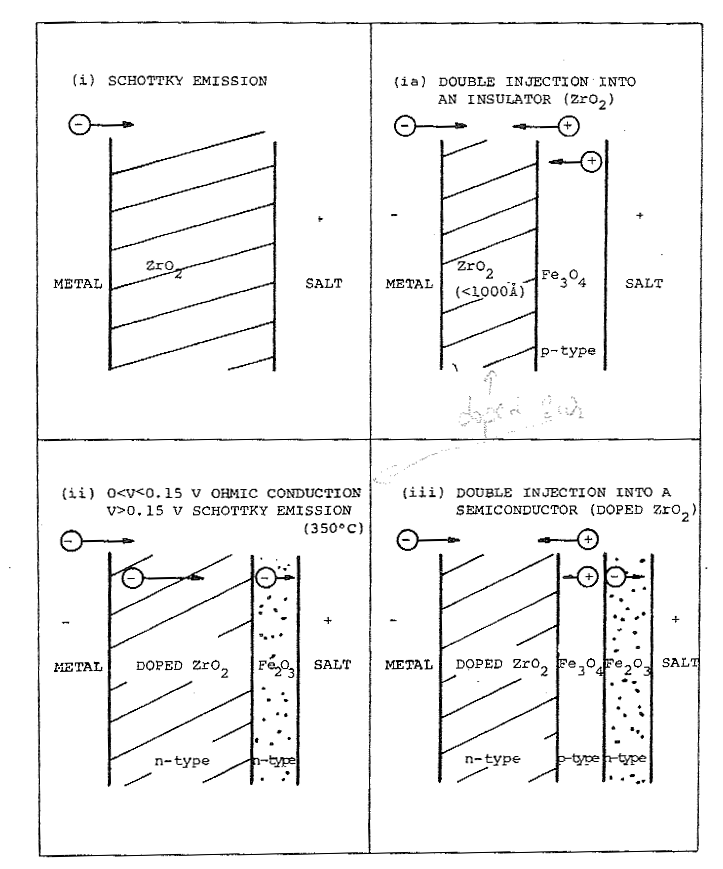
\includegraphics[width=0.9\textwidth]{Shirvington_1970-Fig12.png}
        \caption[Modèles de couche de zircone sur les phases intermétalliques de l'alliage Zircaloy-2.]{Modèles de couche
        d'oxyde sur les intermétalliques de l'alliage Zircaloy-2 \citep{Shirvington1970-1}.}
        \label{fig:shirvington_oxide_structures}
    \end{figure}

    L'auteur insiste sur le fait que la présence de l'oxygène ainsi que le potentiel du métal ont un effet fort sur la
    conductivité de la zircone lorsque de la magnétite peut cristalliser en surface. En effet, le fluide caloporteur
    d'un REB contient très souvent du fer sous forme ionique provenant des pièces de structure de la cuve
    \citep{IAEA1993, IAEA1998, IAEA2011}. Cependant, les dépôts de couleur rouge/orange (appelés CRUD) habituellement observés en
    réacteur sont majoritairement composés d'hématite \citep{Edsinger2004}.
    
    Enfin, l'auteur rappelle que
    l'accélération de la cinétique d'oxydation ne dépend pas seulement de la conduction électronique mais également du
    transport de matière dans la couche de zircone.      
   
   
   
    \subsubsection{Processus limitant}\label{subsubsec:rate_limiting}
         
    La détermination du processus limitant sur la base de mesures séparées des coefficients de diffusion de l'oxygène et de la
    conductivité électronique de la couche de zircone n'est pas simple à réaliser. Comme mentionné précédemment, les deux
    processus sont en balance. Dans le cas où les deux processus n'évoluent pas à la même vitesse dans les
    premiers instants de l'oxydation, une différence de potentiel apparaît entre l'interface interne et l'interface
    externe. Cette dernière accélère le processus le plus lent et ralentit le plus rapide. Les courbes de polarisation
    anodiques et cathodiques permettent d'avoir une estimation du processus limitant dans des conditions expérimentales
    données.

%    Mesurer le potentiel qui apparaît dans la couche d'oxyde n'est simple à réaliser sans perturber la réaction
%    d'oxydation. La figure \ref{fig:potential_drop_Zy2} montre les mesures expérimentales obtenues par \citet{Cox1969}
%    en bain de sel fondu sur du Zy2. Le potentiel à l'interface métal/oxyde diminue vers de potentiel plus cathodiques
%    lors des premiers instants de la croissance de la couche d'oxyde. Cette diminution a été attribuée à la formation d'oxyde de fer en
%    surface des intermétalliques \citep{Shirvington1970, Shirvington1970-1}.

%    \begin{figure}[!htb]
%        \centering
%        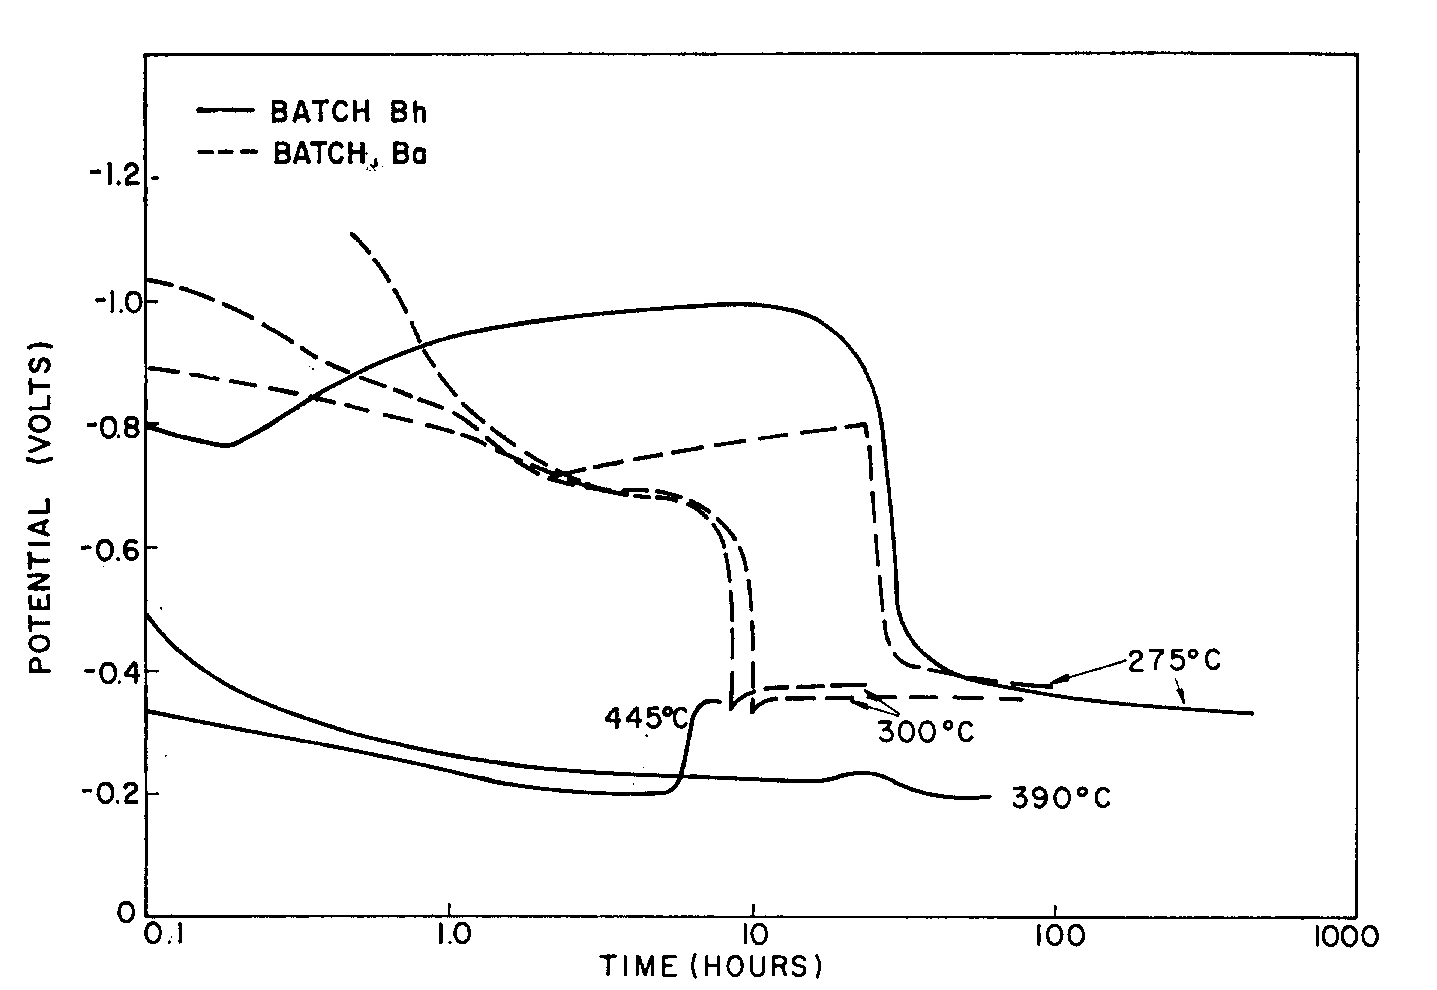
\includegraphics[width=0.45\textwidth]{Cox_1969-Fig4.png}
%        \caption[Evolution du potentiel de l'alliage Zircaloy-2 en bain de sel fondu.]{Evolution du potentiel de l'alliage
%    Zircaloy-2 en bain de sel fondu \citep{Cox1969}.}
%        \label{fig:potential_drop_Zy2}
%    \end{figure}


    Il est fort probable que la conduction électronique pilote la cinétique d'oxydation dans les premiers instants de la
    croissance de la couche de zircone. Cette dernière semble devenir plus conductrice à cause de la contribution des
    phases intermétalliques. Lorsqu'une certaine épaisseur d'oxyde est atteinte, les résistivités électronique et
    ionique semblent plus équilibrées.  La figure \ref{fig:oxide_film_diagram} schématise les différents processus
    intervenants dans l'oxydation de l'alliage Zircaloy-2 au niveau de la couche de zircone lors du régime de
    pré-transition. Cette figure met en lumière la dualité du transport ionique et du transport électronique qui
    doivent être en équilibre afin de maintenir l'électroneutralité dans la couche de zircone.
    
    \begin{figure}[H]
        \centering
        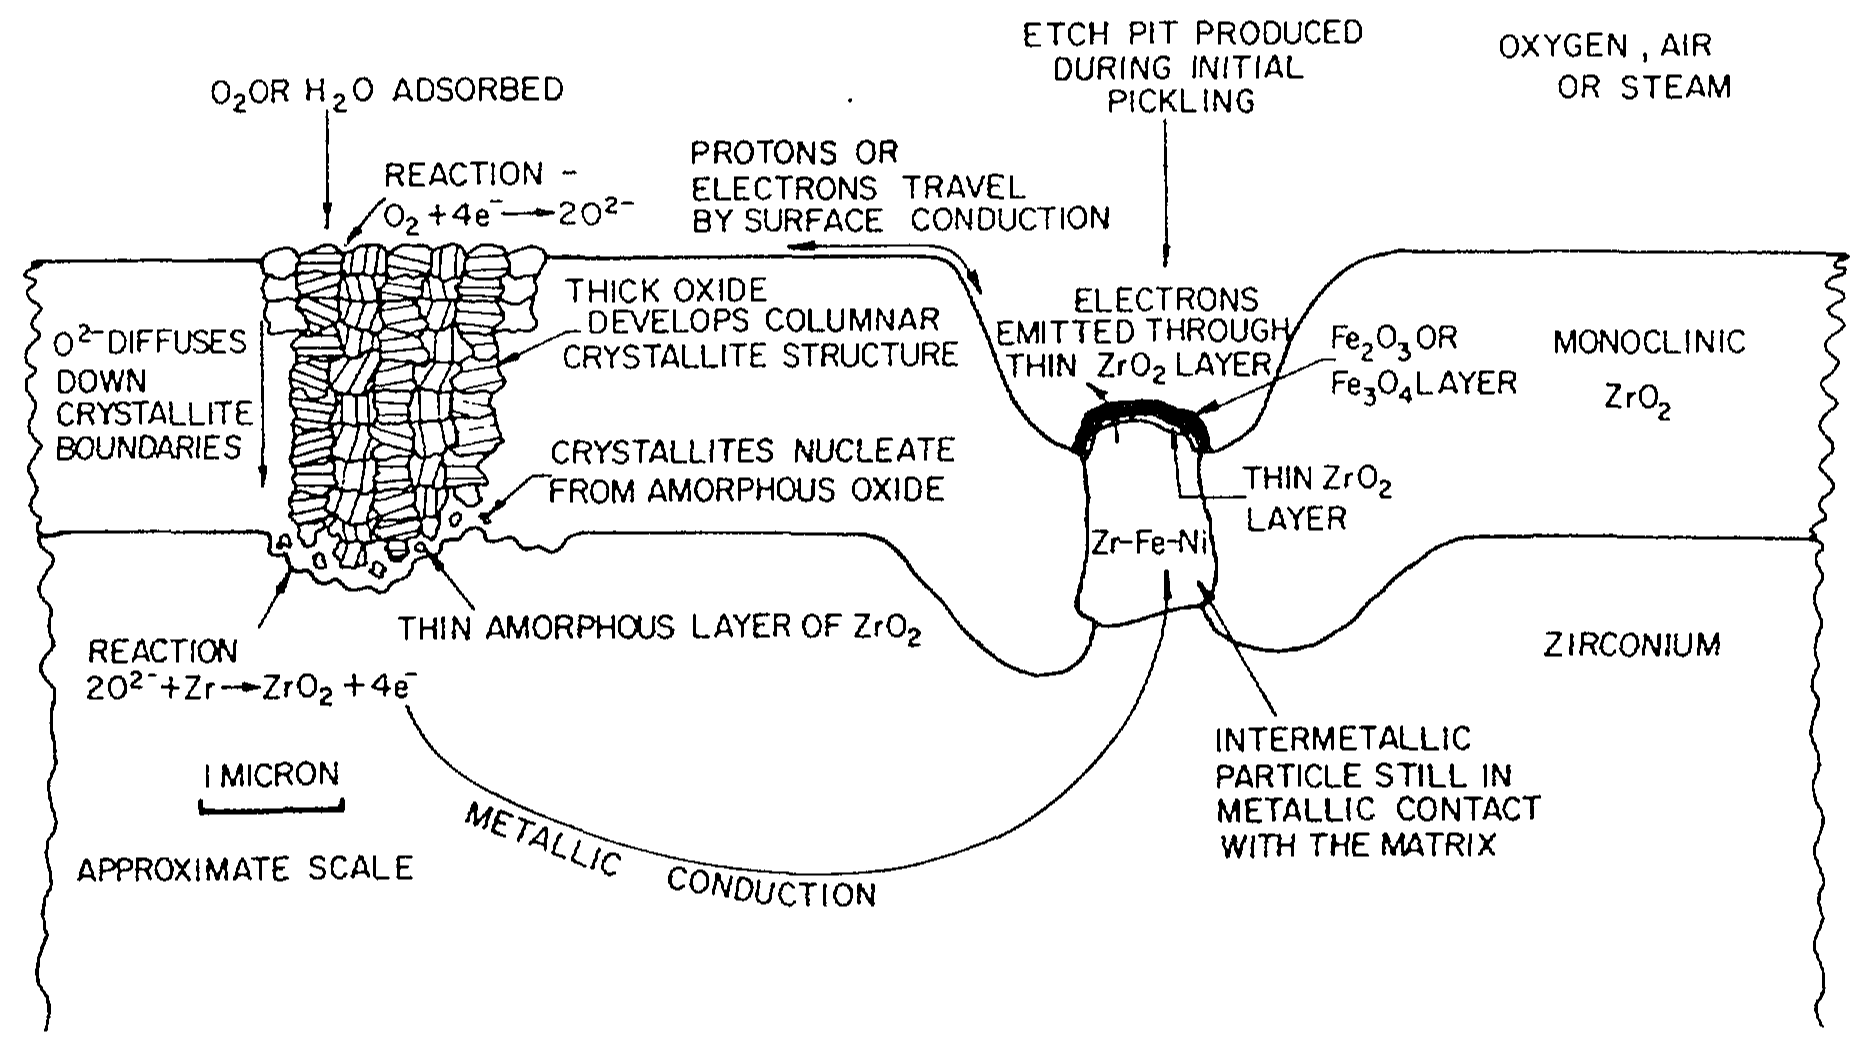
\includegraphics[width=0.95\textwidth]{IAEA_1993_Fig2_17.png}
        \caption[Représentation schématique de la couche de zircone se formant sur l'alliage Zircaloy-2 et des différents
    processus se déroulant lors de l'oxydation.]{Représentation schématique de la couche de zircone se formant sur
    l'alliage Zircaloy-2 et des différents processus se déroulant lors de l'oxydation \citep{IAEA1998}.}
        \label{fig:oxide_film_diagram}
    \end{figure}


    \subsection{Oxydation sous irradiation}\label{subsec:with_irradiation}

    L'impact de l’irradiation sur la cinétique l'oxydation du zirconium n'est pas encore parfaitement connu
    \citep{IAEA1998}. Cependant, un certain nombre de résultats expérimentaux sont disponibles et permettent d'avoir un aperçu de
    l'effet de l'irradiation. 
    
    En première approximation, l'irradiation des matériaux présente dans un coeur de réacteur est due à deux
    types de rayonnements: un rayonnement \emph{neutronique} et un rayonnement électromagnétique $\gamma$, s'y ajoute le
    rayonnement \emph{Cherenkov}, un rayonnement électromagnétique secondaire dans le domaine des UV. 
    Ce rayonnement est liée aux électrons produits par la diffusion de \emph{Compton} des rayonnements $\gamma$ sur les
    matériaux de structure. 
    
    L'irradiation par des neutrons rapides favorise la dissolution des phases intermétalliques et ainsi redistribue les
    éléments d'alliage dans la matrice $\alpha$ \citep{Vizcaino2008, Garzarolli2002}. 
    Cette dissolution est susceptible de doper la couche de zircone qui va se former autour des phases intermétalliques,
    ce qui peut induire une augmentation de la conduction
    électronique comme suggéré dans le paragraphe \ref{subsubsec:charge_carrier}.
    
    Travailler en laboratoire avec des rayonnements
    neutroniques nécessitent des moyens lourds et coûteux. On simule quelquefois l'effet d'une
    irradiation neutronique en la remplaçant par des atomes lourds tels que le xénon.
    \citet{Bererd2005} ont irradié une couche de zircone avec des atomes de Xe  
    ayant une énergie de 64.5 MeV et un flux de \SI{2.6e10}{\per\square\centi\meter\per\second}. La figure
    \ref{fig:Bererd_diffusion_increase} montre que l'irradiation peut engendrer une augmentation du coefficient de
    diffusion de plusieurs ordres de grandeur à \SI{300}{\degreeCelsius}. Cependant, il ne semble pas y avoir peu de preuves
    définitives d'un lien direct entre l'accélération de la cinétique de corrosion et l'augmentation des coefficients de
    diffusion de l'oxygène dans la couche de zircone \citep{IAEA1993, IAEA1998}.
    \citet{Simeone2000, Simeone2002} ont mis en évidence des
    changements de phase locaux dans la couche de zircone lorsque celle-ci est irradiée avec des atomes de Xe.
    L'irradiation avec des particules lourdes crée des défauts dans la couche favorisant la stabilisation de la phase
    quadratique. Cette transformation s'accompagne d'une augmentation des contraintes dans la couche
    de zircone.

    \begin{figure}[H]
        \centering
        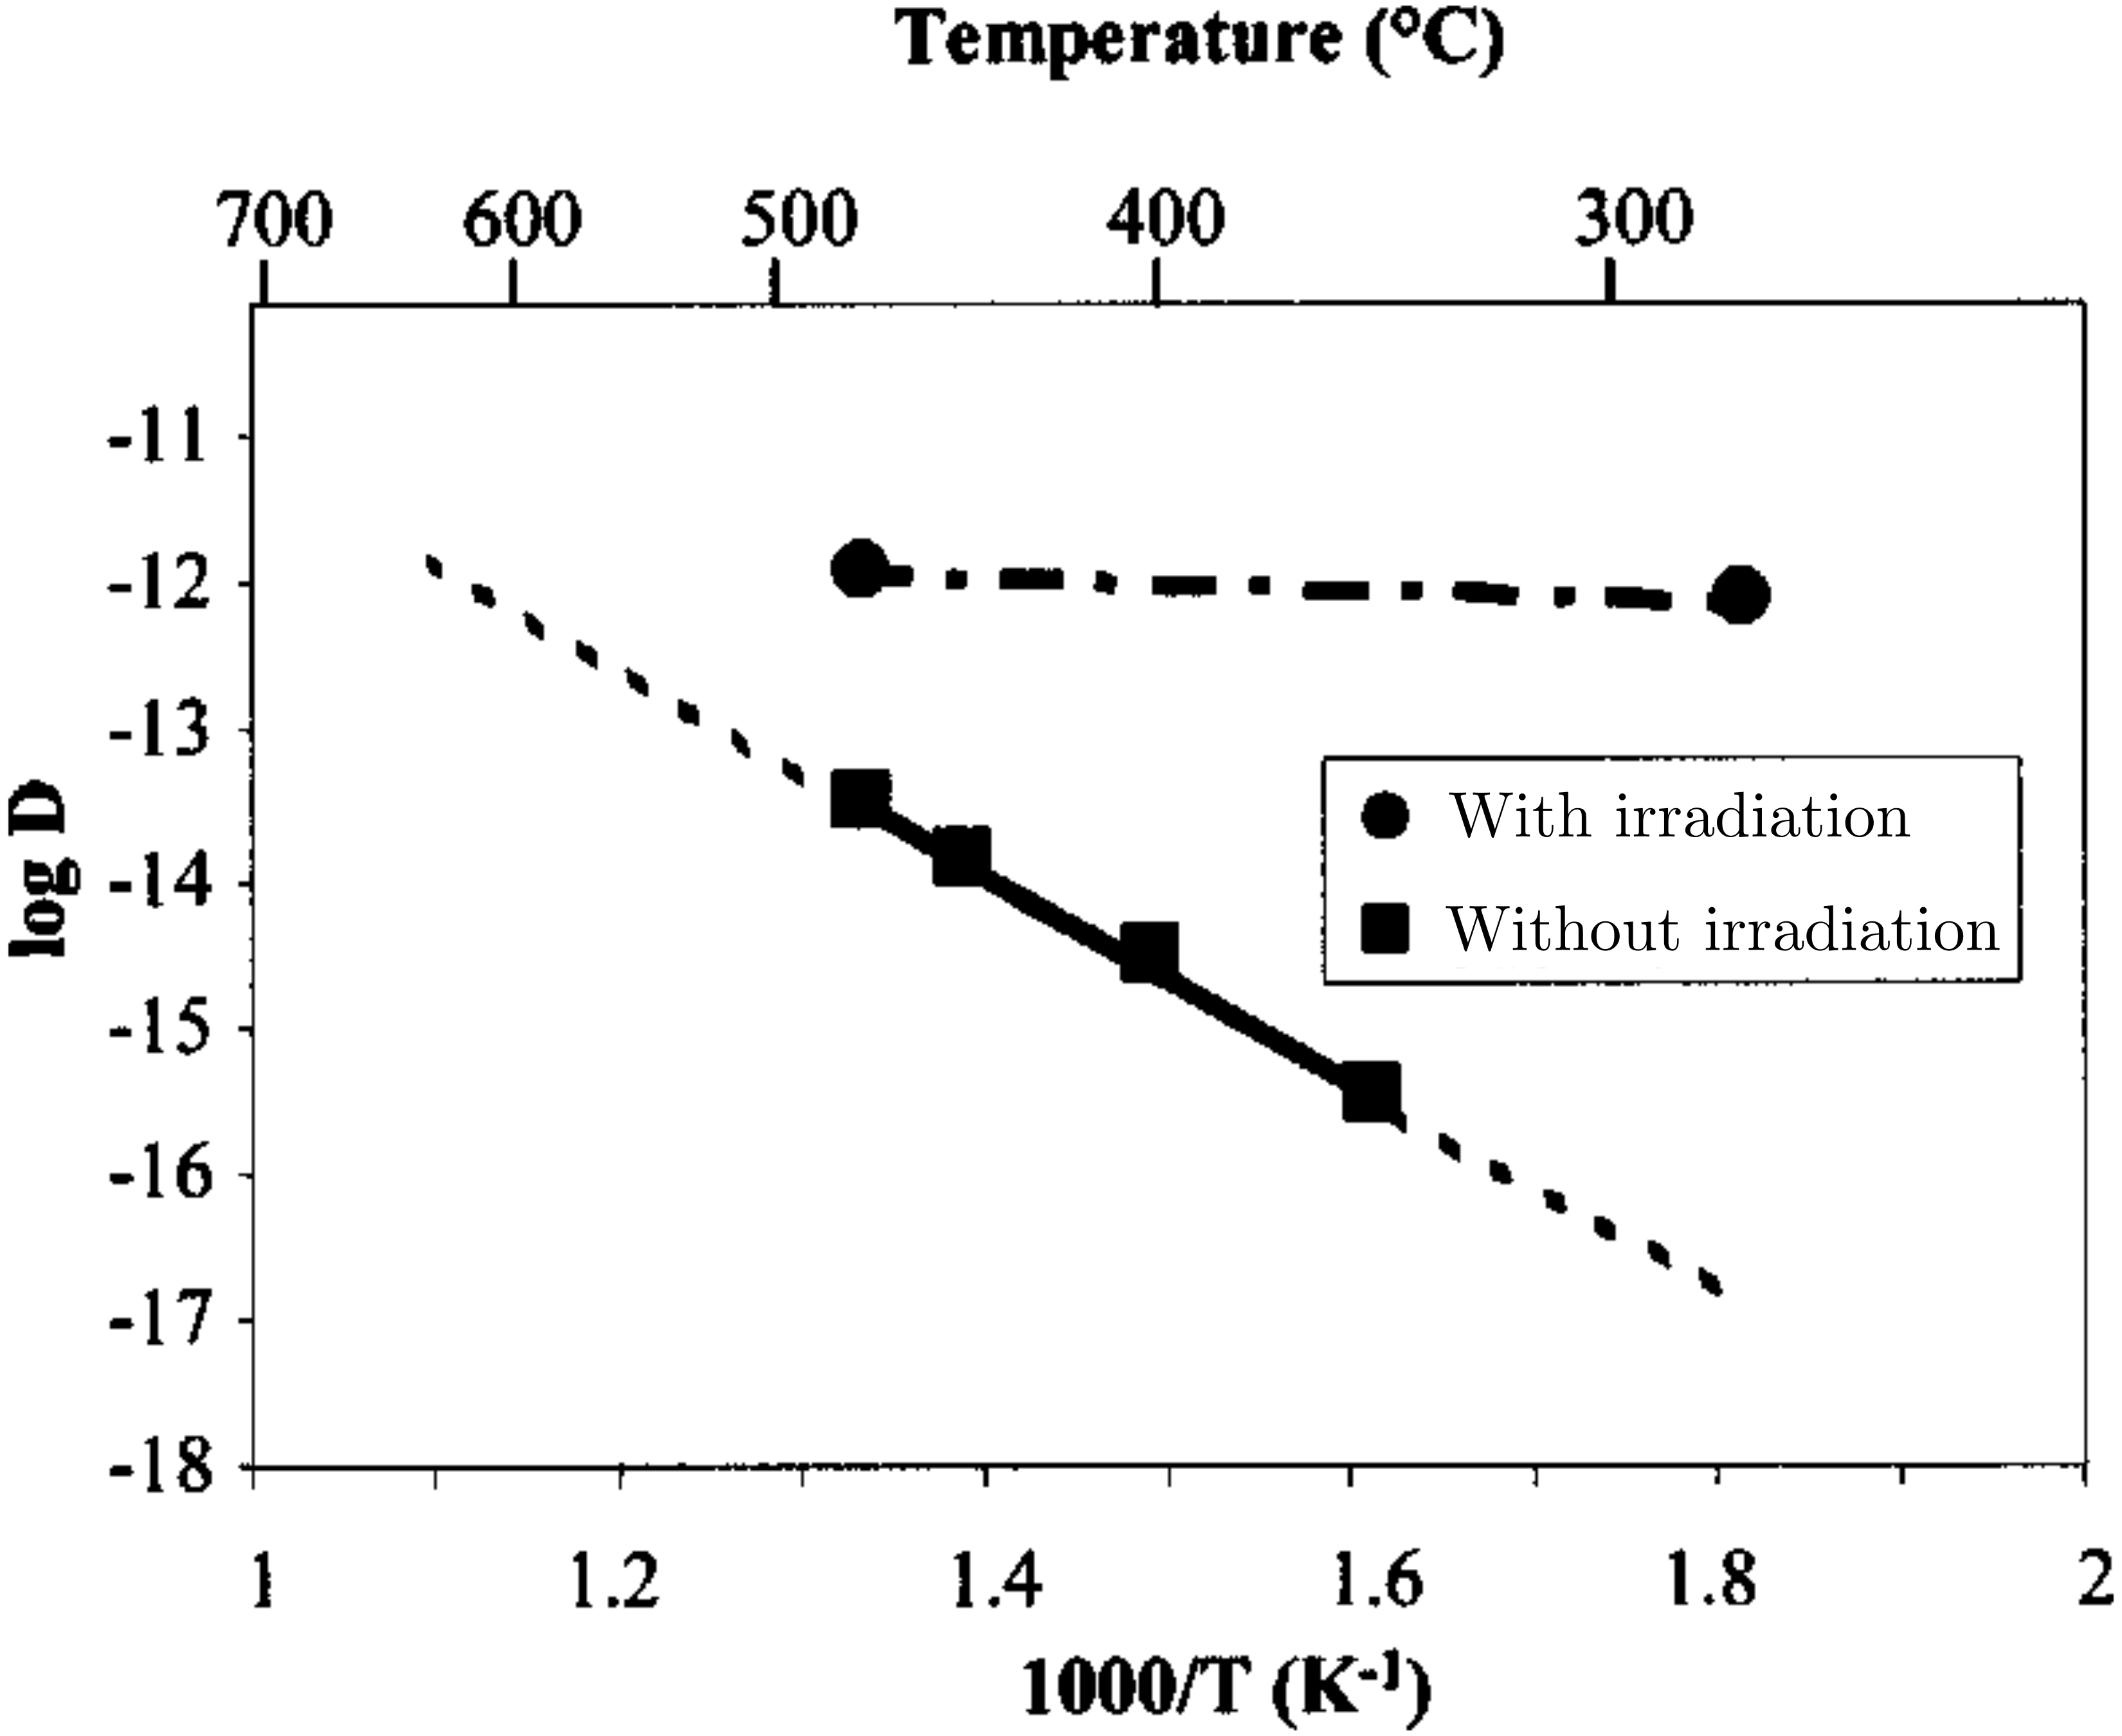
\includegraphics[width=0.65\textwidth]{Bererd_2005-Fig11-redraw.png}
        \caption[Courbe d'Arrhenius du coefficient de diffusion de l'oxygène dans la zircone.]{Courbe d'Arrhenius du
        coefficient de diffusion de l'oxygène dans la zircone \citep{Bererd2005}.}
        \label{fig:Bererd_diffusion_increase}
    \end{figure}


    L'irradiation par des rayonnements $\gamma$ peut augmenter de quelques ordres de grandeur la conductivité
    électronique de
    céramiques considérées isolantes telle que l'alumine \citep{Shikama1994}. \citet{Howlader1999} se sont intéressés à la
    conductivité de la zircone sous irradiation d'électrons de 1~MeV. L'auteur note une forte augmentation de
    la conductivité comme illustré sur la figure \ref{fig:conductivty_electron_beam}, et que l'impact de
    l'irradiation d'électrons diffère selon la nuance considérée. 


    \begin{figure}[H]
        \centering
        \begin{subfigure}[b]{0.48\textwidth}
            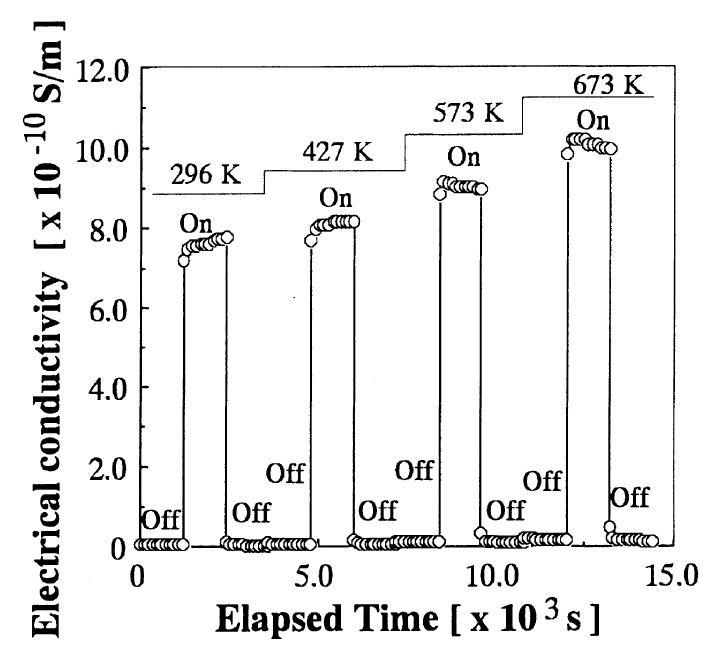
\includegraphics[width=\textwidth]{Howlader_1999-Fig6a.png}
            \caption{}
            \label{subfig:conductivity_gamma_Zy2}
        \end{subfigure}
        \quad
        \begin{subfigure}[b]{0.48\textwidth}
            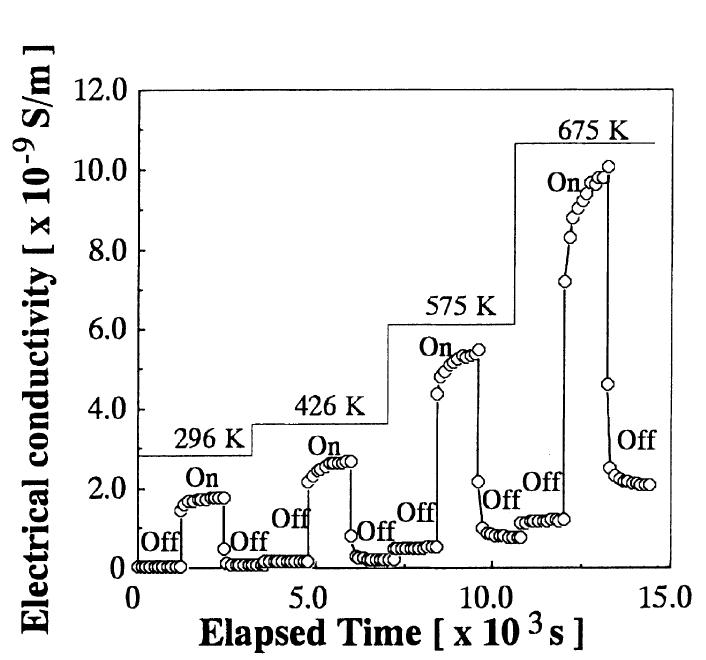
\includegraphics[width=\textwidth]{Howlader_1999-Fig6b.png}
            \caption{}
            \label{subfig:conductivity_gamma_improved_Zy2}
        \end{subfigure}
        \quad
        \begin{subfigure}[b]{0.48\textwidth}
            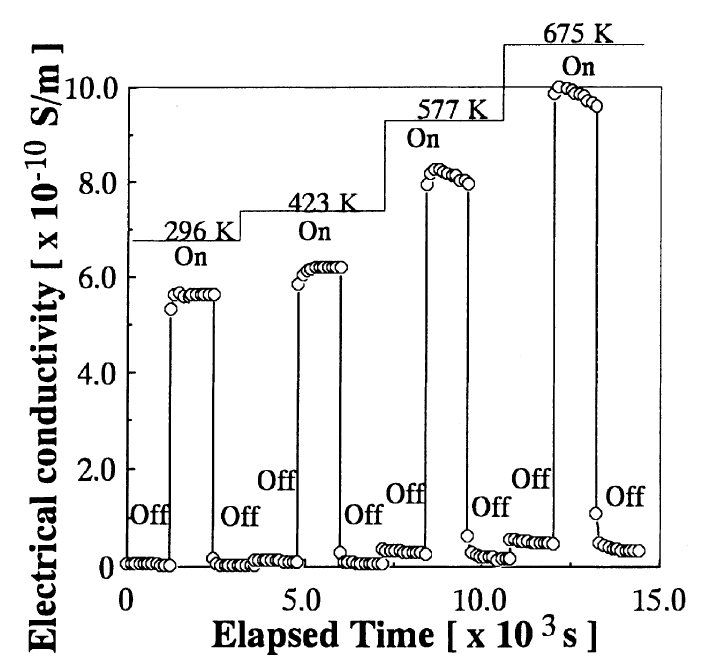
\includegraphics[width=\textwidth]{Howlader_1999-Fig6c.png}
            \caption{}
            \label{subfig:conductivity_gamma_Zy4}
        \end{subfigure}
    \caption[Effet de l'irradiation avec des électrons (1 MeV avec un flux de \num{1.4e18}~$e m^{-2} s^{-1}$) sur la conductivité électronique
    de la couche de zircone sur l'alliage: a) Zircaloy-2, b) Zircaloy-2 modifié et c) Zircaloy-4.]
    {Effet de l'irradiation avec des électrons (1 MeV avec un flux de \num{1.4e18}~$e m^{-2} s^{-1}$) sur la conductivité électronique
    de la couche de zircone sur l'alliage: a) Zircaloy-2, b) Zircaloy-2 modifié et c) Zircaloy-4 \citep{Howlader1999}.}
    \label{fig:conductivty_electron_beam}
    \end{figure} 
    
    Le rayonnement neutronique ainsi que le rayonnement $\gamma$ sont également responsables de la radiolyse de l'eau
    \citep{Cowan2011}. Les réactions chimiques pouvant se produire entre les différents produits de radiolyse sont
    nombreuses \citep{Trupin-Wasselin2000, Auclair2001}. Parmi les produits de radiolyse primaire, c'est-à-dire ceux
    qui ont une durée de vie assez longue pour réagir chimiquement (de quelques nanosecondes à la milliseconde \citep{Trupin-Wasselin2000}), on trouve les espèces $e^-_{aq}$, $HO^{\bullet}$,
    $H^{\bullet} $,  $HO_2^{\bullet}$ et $H_2O_2$. Le peroxyde d’hydrogène possède la plus longue durée de vie et
    reste par conséquent le produit majoritaire de la radiolyse de l'eau. Néanmoins, sa concentration n'est pas
    identique sur toute la longueur de la gaine comme illustré sur la figure \ref{fig:radiloytic_species_profil} et les
    concentrations locales peuvent différer des valeurs en volume notamment au niveau des grilles de maintien. A cette 
    hétérogénéité de concentration de peroxyde d'hydrogène correspond une hétérogénéité de pouvoir oxydant de
    l'environnement le long de la gaine.  

    \begin{figure}[H]
        \centering
        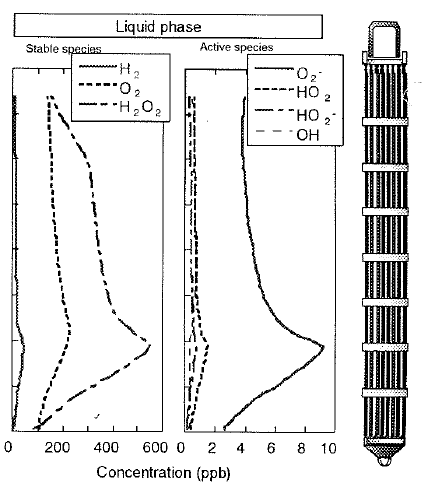
\includegraphics[width=0.75\textwidth]{Adamson_2002_Fig1-3-H2O2.png}
        \caption[Profil de concentration calculé des produits de radiolyse le long des gaines.]
        {Profil de concentration
        calculé des produits de radiolyse le long des gaines \citep{Adamson2002}.}
        \label{fig:radiloytic_species_profil}
    \end{figure}

    
    Il a été proposé que la présence de peroxyde d'hydrogène peut engendrer une dissolution locale de la couche de zircone
    \citep{IAEA1997}. \citet{Nishino1997} montrent que de la zircone massive stabilisée à l'yttrium est susceptible d'être
    dissoute lorsque cette dernière est irradiée par un rayonnement $\gamma$ à \SI{25}{\degreeCelsius} comme illustré
    par la figure \ref{subfig:Nishino_gamma_effect_YSZ}. La figure \ref{subfig:Nishino_gamma_effect_Zy2}, qui montre
    les prises de masse mesurées sur un alliage de Zircaloy-2 sous irradiation $\gamma$ à
    \SI{288}{\degreeCelsius}, semble confirmer cette observation.

    \begin{figure}[H]
        \centering
        \begin{subfigure}[b]{0.42\textwidth}
            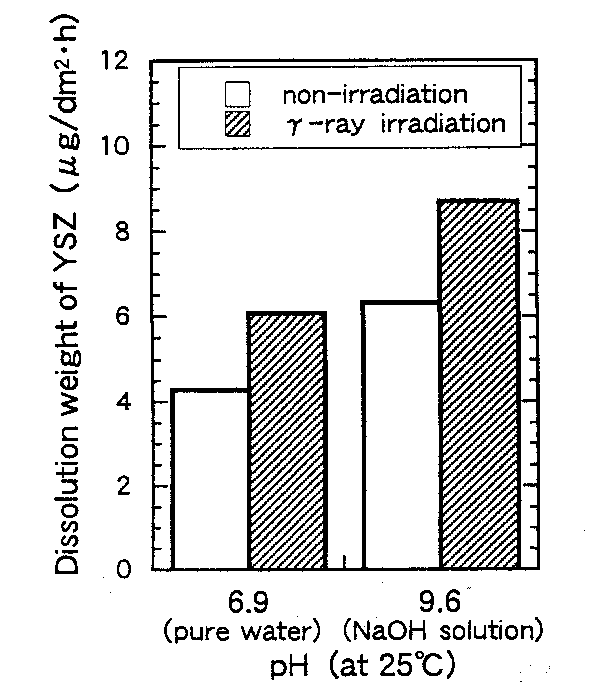
\includegraphics[width=\textwidth]{Nishino_1997-Fig8.png}
            \caption{}
            \label{subfig:Nishino_gamma_effect_YSZ}
        \end{subfigure}
        \quad
        \begin{subfigure}[b]{0.48\textwidth}
            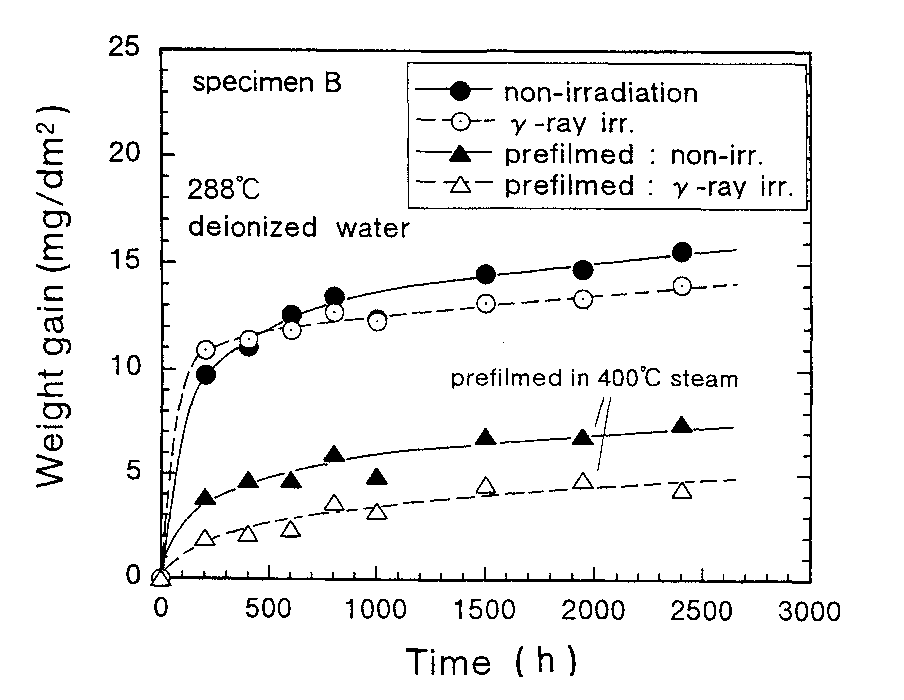
\includegraphics[width=\textwidth]{Nishino_1997-Fig3.png}
            \caption{}
            \label{subfig:Nishino_gamma_effect_Zy2}
        \end{subfigure}
        \caption[Effet de l'irradiation $\gamma$: 
        a) perte de masse de la zircone stabilisée à l'yttrium dans l'eau à \SI{25}{\degreeCelsius} sous irradiation,
        b) prise de masse de alliage Zircaloy-2  dans de l'eau pure à \SI{288}{\degreeCelsius} sous irradiation
    $\gamma$.]
        {Effet de l'irradiation $\gamma$: 
        a) perte de masse de la zircone massive stabilisée à l'yttrium dans l'eau à \SI{25}{\degreeCelsius} sous irradiation,
        b) prise de masse de alliage Zircaloy-2  dans de l'eau pure à \SI{288}{\degreeCelsius} sous irradiation $\gamma$
        \citep{Nishino1997}.}
        \label{fig:Nishino_Gamma_Effect}
    \end{figure}

    
    Par ailleurs, \citet{Cox1989} se sont intéressés à l'impact de l'illumination UV avec une lampe Xe 150W sur l'oxydation
    de l'alliage Zircaloy-2 à température ambiante.
    Ces auteurs montrent que l'illumination UV peut engendrer une légère augmentation de
    l'épaisseur de la couche de zircone sous une forte polarisation anodique. 
    %Cependant, l'utilisation de solution très
    %acide ou très basique ne permet pas de conclure si l'augmentation d'épaisseur serait également observée à pH neutre. 
    %Plus récemment, \citet{Goossens1996} ont étudié l'impact de la lumière UV sur une couche de zircone formée
    %anodiquement sur du zirconium
    %pure avec un potentiel imposé de \SI{12}{\volt}. La longueur d'onde de la lumière UV utilisée était de
    %\SI{220}{\nano\meter} avec une puissance de \SI{452}{\micro\watt\per\square\centi\meter}.
    %L'épaisseur de la couche de zircone a augmentée de \SI{1}{\nano\meter} pour une durée d'illumination d'environ
    %\SI{15}{\minute}. L'augmentation d'épaisseur a été attribuée à une diminution de l'intensité du champ électrique
    %dans la couche de zircone.

    L'étude de l'effet de l'irradiation n'est pas simple car elle peut agir simultanément sur le transport ionique et
    le transport électronique de la couche de zircone. Les effets sur le transport ionique et électronique peuvent être
    quantifiés sur les branches anodiques et cathodiques des courbes de polarisation, respectivement. 
    \citet{Cox1968} a proposé une synthèse des modifications hypothétiques subies par les branches anodiques et
    cathodiques sous irradiation en fonction de l'environnement comme illustré sur la figure
    \ref{fig:irradiation_effect_IE_plots}. Les courbes de polarisations anodiques et cathodiques classiquement mesurées en
    autoclave sur les alliages de zirconium sont présentées en figure \ref{fig:irradiation_effect_IE_plots}a).
    La présence de l'irradiation seule, illustrée par la figure \ref{fig:irradiation_effect_IE_plots}b), 
    impacterait seulement la branche anodique et induirait une faible augmentation du courant de corrosion, 
    alors que la présence supplémentaire d'oxygène, illustrée par la figure \ref{fig:irradiation_effect_IE_plots}c), impacte 
    les deux branches induisant ainsi une forte augmentation du courant de corrosion. La figure
    \ref{fig:irradiation_effect_IE_plots}d) illustre que la pré-oxydation permet de diminuer le courant de corrosion.

    En prenant en compte la possibilité d'avoir des branches anodiques et
    cathodiques qui différent à l'échelle locale par rapport à l'échelle de la gaine entière, différents types de corrosion
    sous irradiation peuvent être observés. En effet, trois types majeurs de corrosion ont été
    définis: \emph{corrosion uniforme}, \emph{corrosion nodulaire} et la \emph{Shadow Corrosion}.

    \begin{figure}[H]
        \centering
        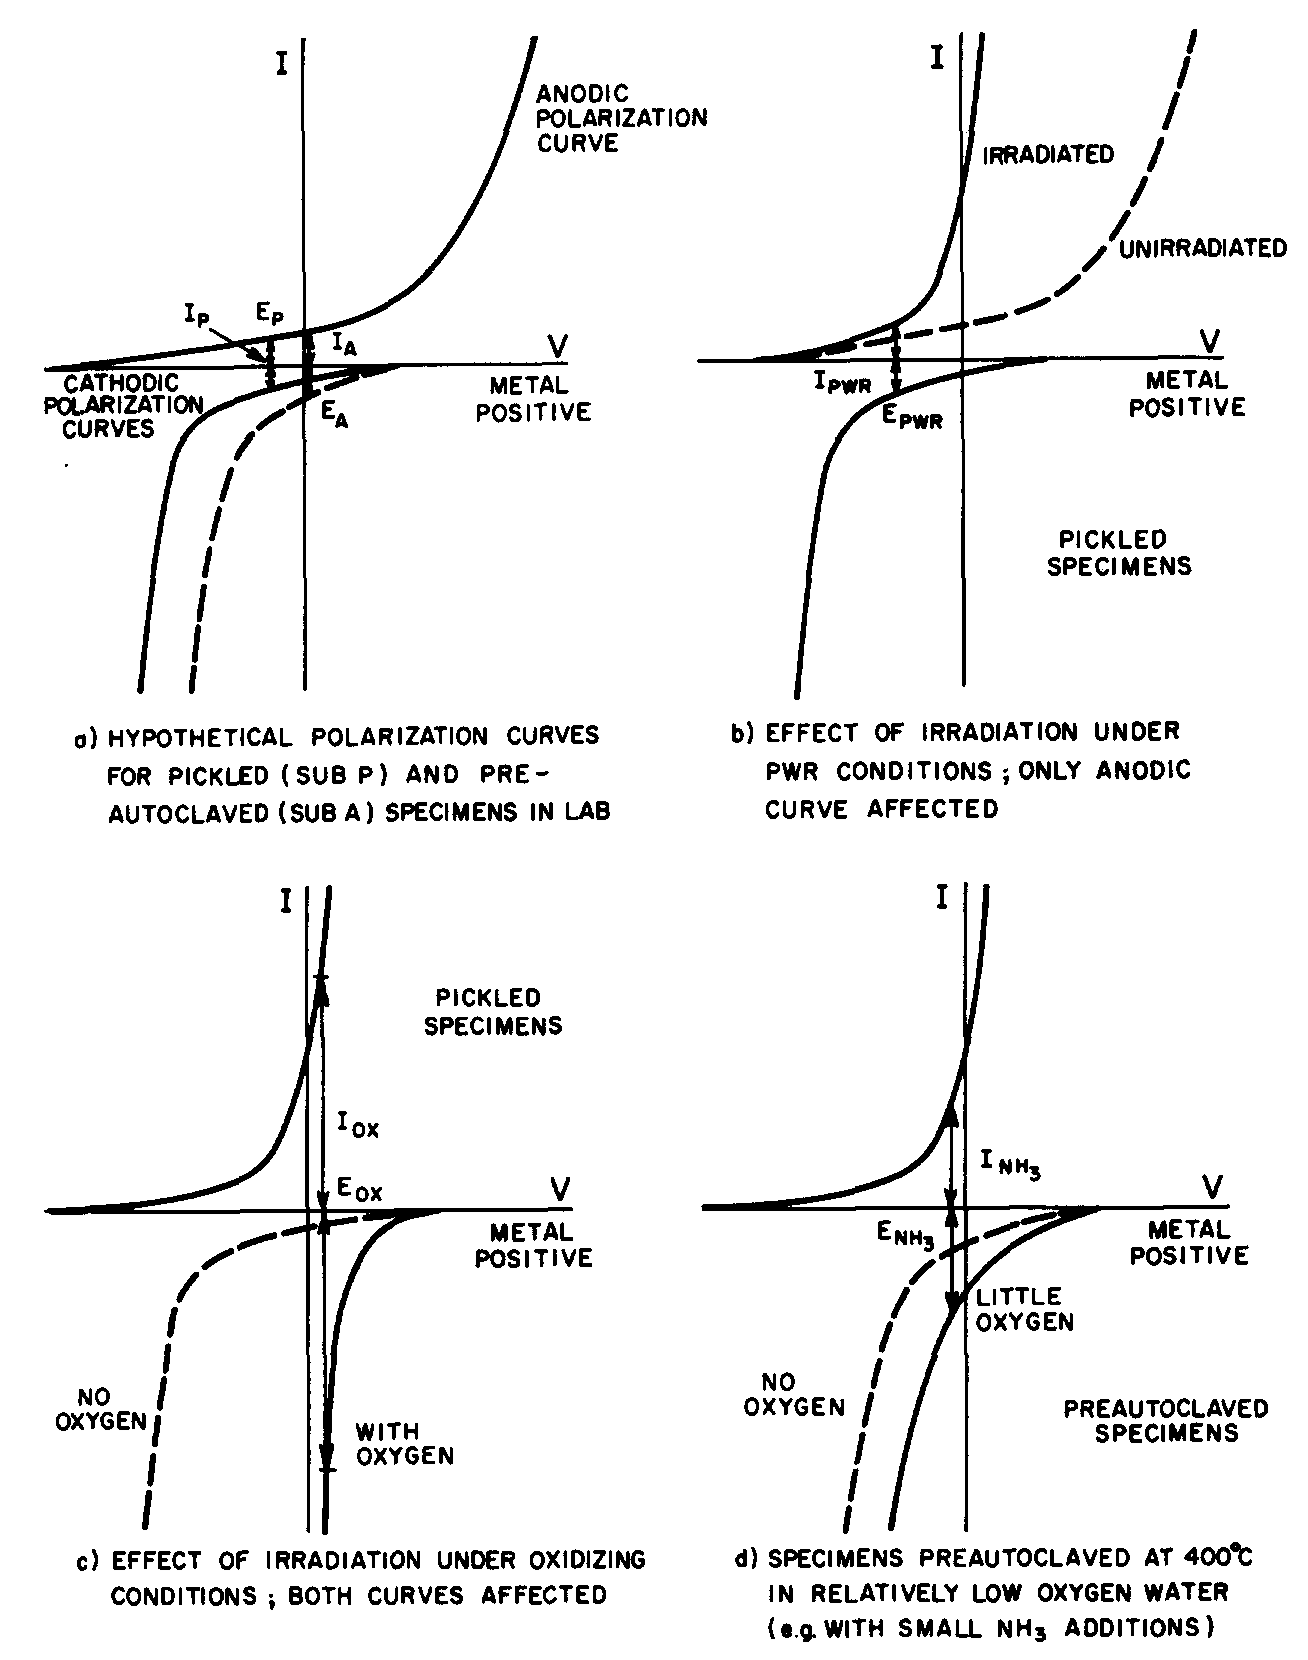
\includegraphics[width=0.9\textwidth]{Cox_1968b-Fig32.png}
        \caption[Effets hypothétiques de l'irradiation sur le transport ionique et électronique.]
        {Effets hypothétiques de
    l'irradiation sur le transport ionique (branche anodique) et électronique
        (branche cathodique) \citep{Cox1968-1}.}
        \label{fig:irradiation_effect_IE_plots}
    \end{figure}
    

    
    \subsection{Points clés de l'oxydation des alliages de zirconium}
        
        Moyennant quelques approximations, les mesures expérimentales de cinétique de prise de masse peuvent être
        converties en épaisseur de couche de zircone équivalente et en densité de courant d'oxydation équivalente. 

        La cinétique d'oxydation du Zircaloy-2 est relativement lente en autoclave. En effet, après un an d'oxydation en
        autoclave, la couche de zircone présente une épaisseur de seulement quelques microns. Cela correspond à une
        densité de courant entre 2 et 5 \si{\micro\ampere\per\square\centi\meter} au début de l'oxydation et elle
        atteint environ \SI{0.05}{\micro\ampere\per\square\centi\meter} après un an d'oxydation.

        La cinétique d'oxydation comporte deux régimes distincts (dits \emph{pré-transition} et \emph{post-transition}) séparés par
        une phase de \emph{transition}. La couche de zircone formée lors du 
        régime de pré-transition est plus dense alors que la couche formée lors du régime de post-transition 
        \citep{IAEA1998}. Généralement, la phase de \emph{transition} débute lorsque la couche de zircone atteint
        environ \SI{2}{\micro\meter}. Le profil cinétique d'oxydation du régime de
        \emph{pré-transition} est sub-parabolique alors qu'il est linéaire dans le régime de \emph{post-transition}.

        Les conditions oxydantes lors de la formation de la couche de zircone sont susceptible d'impacter sa
        conductivité en favorisant plus ou moins la dissolution d'éléments plus nobles tels que Fe, Cr et Ni
        pouvant doper la couche de zircone. En effet, la ségrégation de Fe et
        de Ni aux joints de grain de la couche de zircone peuvent favoriser le transport électronique.

        L'accélération de la cinétique d'oxydation ne dépend pas seulement de la conductivité électronique mais
        également de la conductivité ionique car les deux processus sont en équilibre. Dans le cas où les deux processus
        n'évoluent pas à la même vitesse dans les
        premiers instants de l'oxydation, une différence de potentiel apparaît entre l'interface interne et l'interface
        externe. Cette dernière accélère le processus le plus lent et ralentit le plus rapide.
        
        L’irradiation que subissent les matériaux englobe des rayonnements électromagnétiques allant des UV profonds aux
        rayonnements $\gamma$ ainsi que le rayonnement neutronique. Ces rayonnements peuvent impacter le transport ionique
        ainsi que le transport électronique des oxydes formés sur les gaines de confinement et les grilles de maintien. 
        La principale conséquence de l'irradiation est la perturbation de l'équilibre qui s'établit entre le transport
        ionique et le transport électronique afin d'assurer l'électroneutralité dans la couche de zircone. Toutefois, il
        semble y avoir peu de preuves avérées sur le lien direct entre l’accélération de la cinétique de corrosion et 
        l’augmentation des coefficients de diffusion de l’oxygène dans la couche de zircone.
        



%%%%%%%%%%%%%%%%%%%%%%%%%%%%%%%%%%%%%%%%%%%%%%%%%%%%%%%%%%%%%%%%%%%%%%%%%%%%%%%%%%%%%
%%%%%%%%%%%%%%%%%%%%%%%%%%%%%%%%%%%%%%%%%%%%%%%%%%%%%%%%%%%%%%%%%%%%%%%%%%%%%%%%%%%%%
\section{Phénomène de Shadow Corrosion}\label{sec:shadow_corrosion}

La Shadow Corrosion est communément définie comme un phénomène localisé de corrosion aggravée des alliages de zirconium
lorsque ces derniers se trouvent à proximité d'alliages plus \emph{nobles} tels que les alliages de nickel ou les aciers
inoxydables \citep{Chen1994}. Ce phénomène est uniquement observé dans les REB, dont
l'environnement est plus oxydant que dans les REP en raison de teneurs plus élevées
en oxygène et peroxyde d'hydrogène dissous dans l'eau \citep{Adamson2002}.

Pour mémoire, les assemblages de combustibles des REB sont constitués de gaines en alliage de zirconium de type Zircaloy-2
lesquelles sont maintenues par des grilles de maintien faites en alliage base nickel \cite{Garzarolli2011} comme
illustré sur la figure \ref{fig:what_is_shadow_corrosion}a. L'accroissement accéléré de la couche de zircone sur la gaine se situe
dans la zone en vis-à-vis de la grille de maintien. La surépaisseur de la couche de zircone peut atteindre dix fois la
valeur attendue pour une durée d'exposition donnée. Elle se manifeste par un oxyde de couleur blanche qui reproduit
la forme de la pièce en vis-à-vis comme on peut s'en rendre compte sur la figure \ref{fig:what_is_shadow_corrosion}b
\citep{Bischoff2012}.
Les grilles de maintien maintiennent les gaines de confinement à l'aide de ressorts qui sont en contact avec la surface
de ces dernière.
Une représentation schématique de la zone de contact est présentée en figure \ref{fig:what_is_shadow_corrosion}c.
 


    \begin{figure}[H] 
        \centering 
        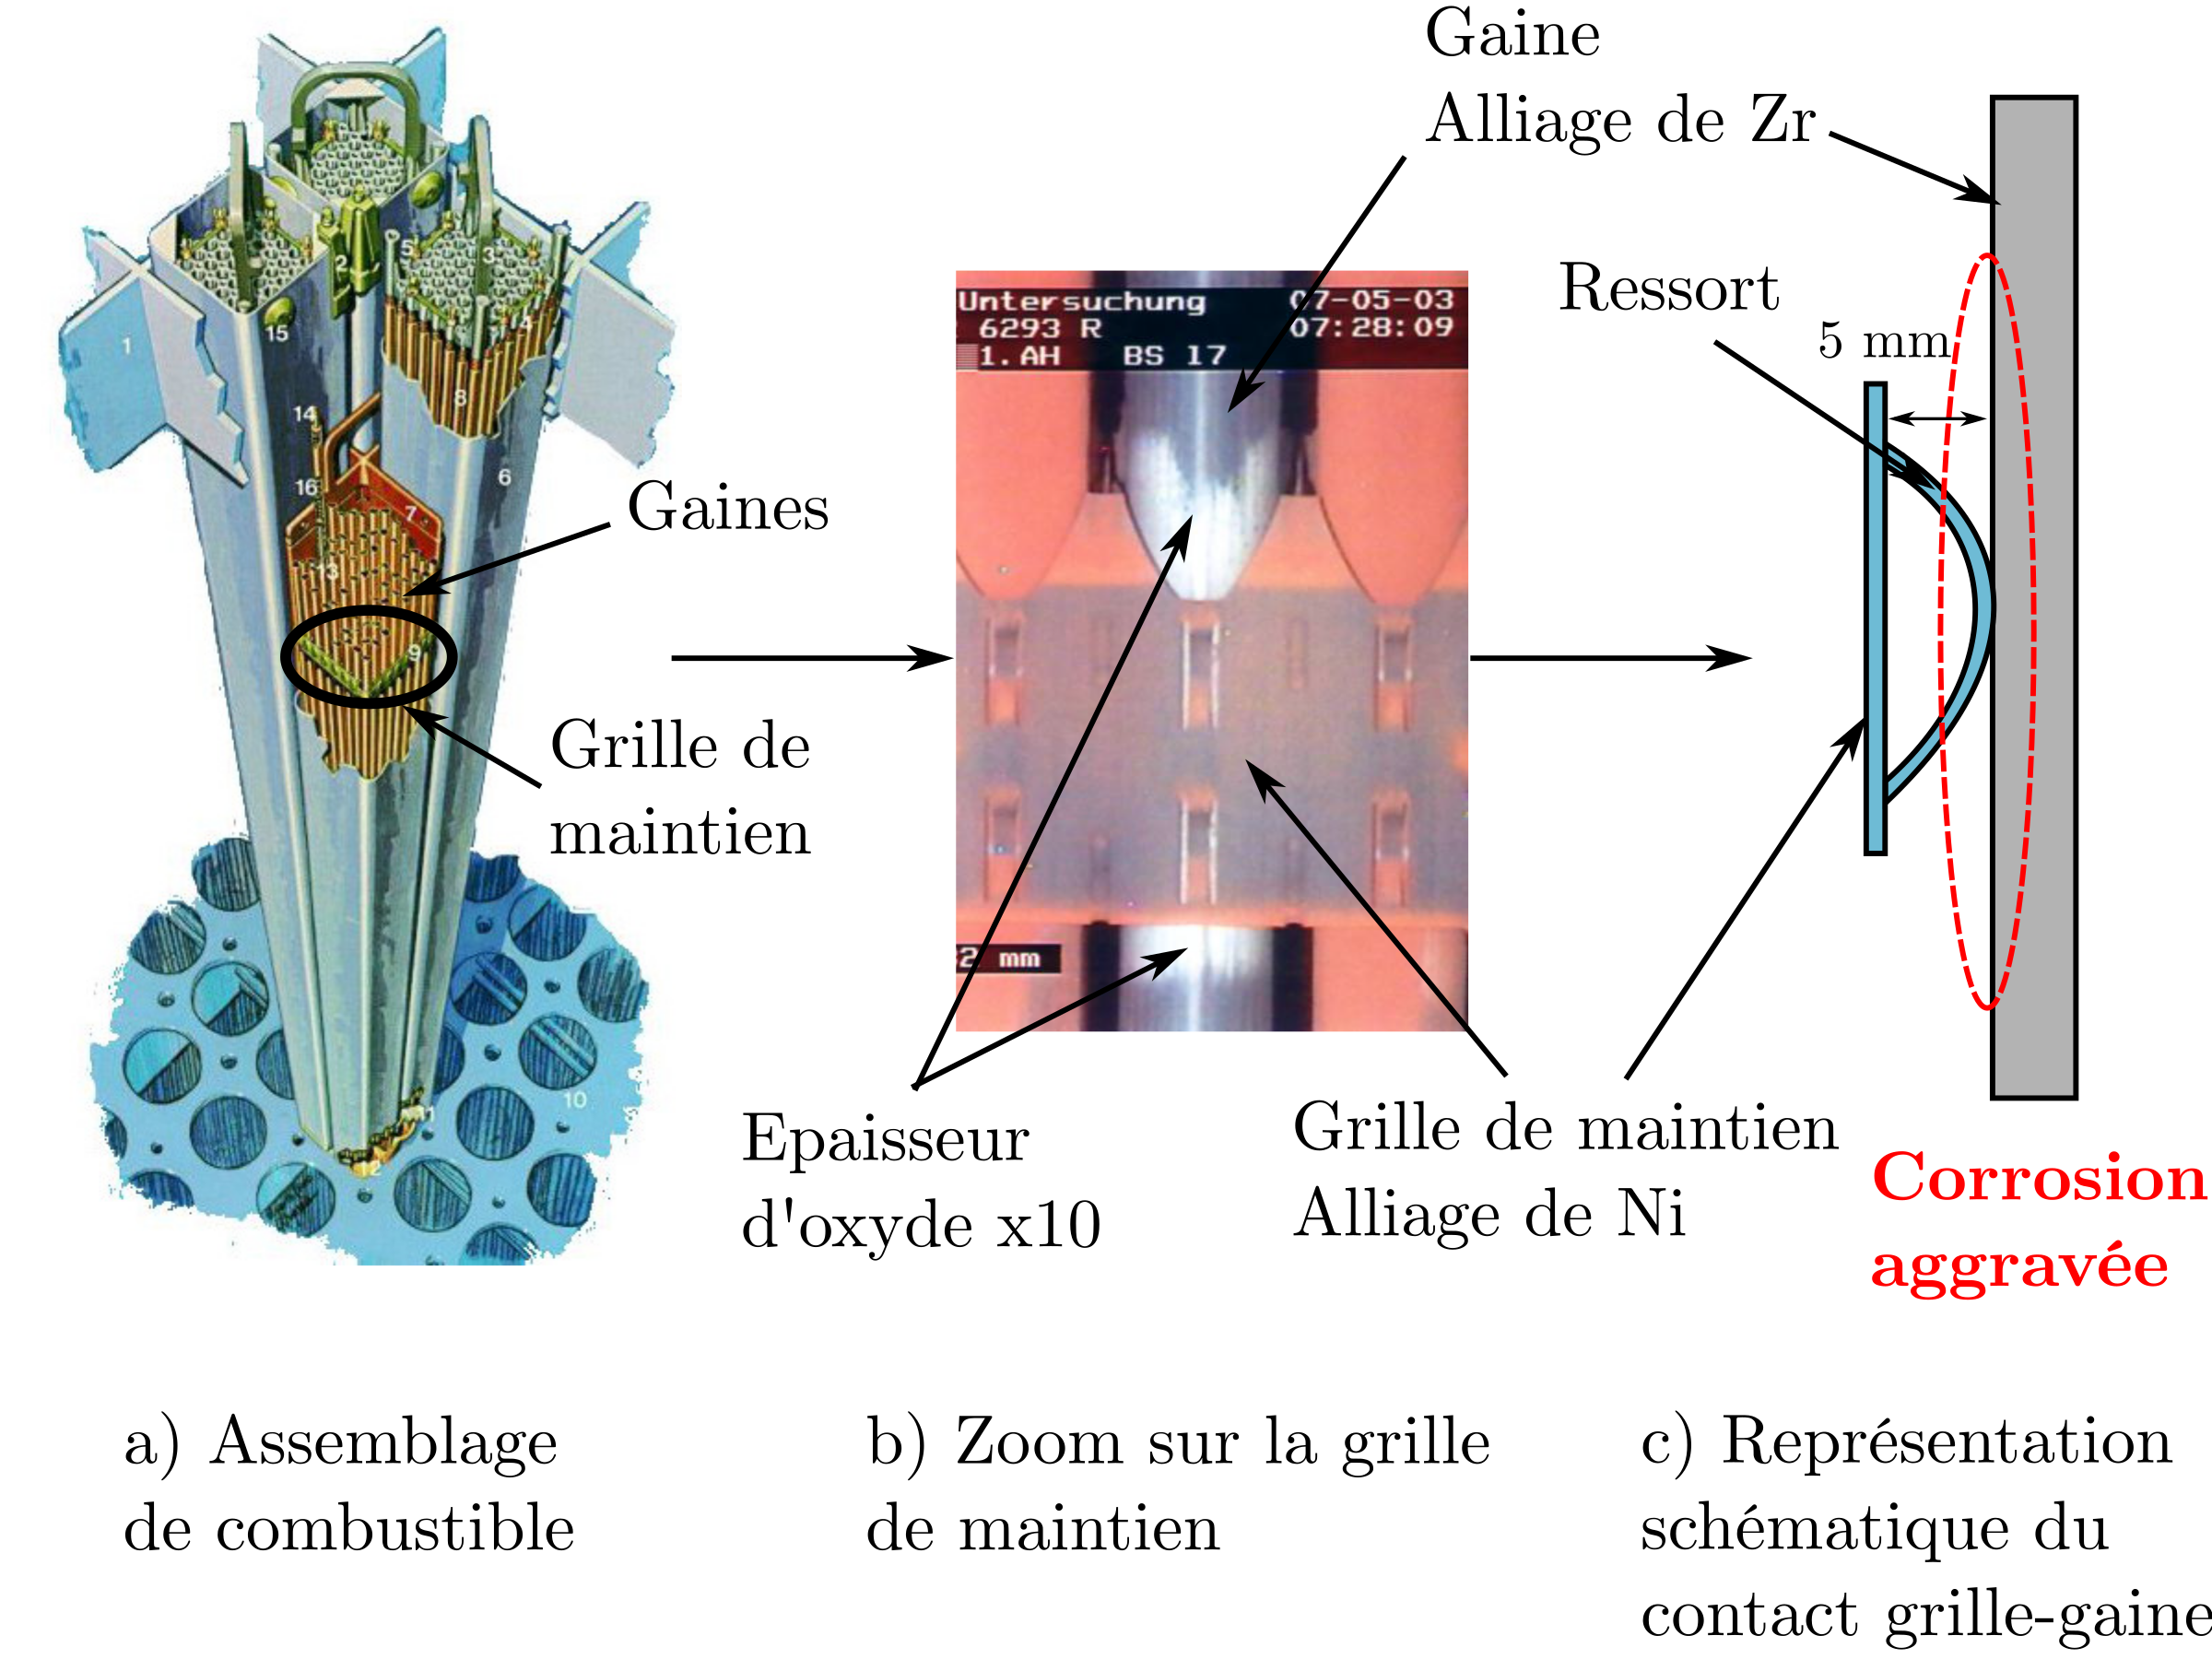
\includegraphics[width=0.95\textwidth]{what_is_shadow_corrosion.png}
        \caption[Schéma du phénomène de Shadow Corrosion]{Représentation schématique de la localisation du phénomène de
     Shadow Corrosion sur les assemblages de combustible dans un REB.} 
        \label{fig:what_is_shadow_corrosion} 
     \end{figure}


Le phénomène de Shadow Corrosion est connu depuis les années 1970. \citet{Johnson1974} ont signalé l’apparition de
corrosion accélérée sur des coupons de zirconium à proximité de pièces en platine dans un réacteur test.
\citet{Trowse1977} ont également observé la présence de corrosion aggravée des gaines de confinement sous les grilles
de maintien dans un réacteur à eau lourde. Cependant, ce phénomène n'a été étudié qu'à partir des années 2000 lorsqu’une
rupture de gaine de confinement s'est produite dans un REB en Suisse (réacteur KKL, Westinghouse, 
figure \ref{fig:fuel_rod_failure_KKL}).
Le mécanisme de rupture a été attribué à une forme aggravée de
Shadow Corrosion au niveau des grilles de maintien \citep{Edsinger2004}, dénommée par la suite ESCC
(Enhanced Spacer Shadow Corrosion).
Le problème a été partiellement résolu en s'appuyant sur les données de fonctionnement du réacteur antérieures à
l'incident, dont l'analyse a conduit au réajustement du ratio de $\frac{[Fe_{aq}]}{[Ni_{aq}]+[Zn_{aq}]}$ 
dans l'eau afin qu'il soit supérieur à 2, à l'augmentation de la teneur en fer dans l'alliage 
de zirconium et au changement d'un paramètre de recuit de l'alliage de zirconium \citep{Edsinger2004}.

         
     \begin{figure}[H] 
        \centering 
        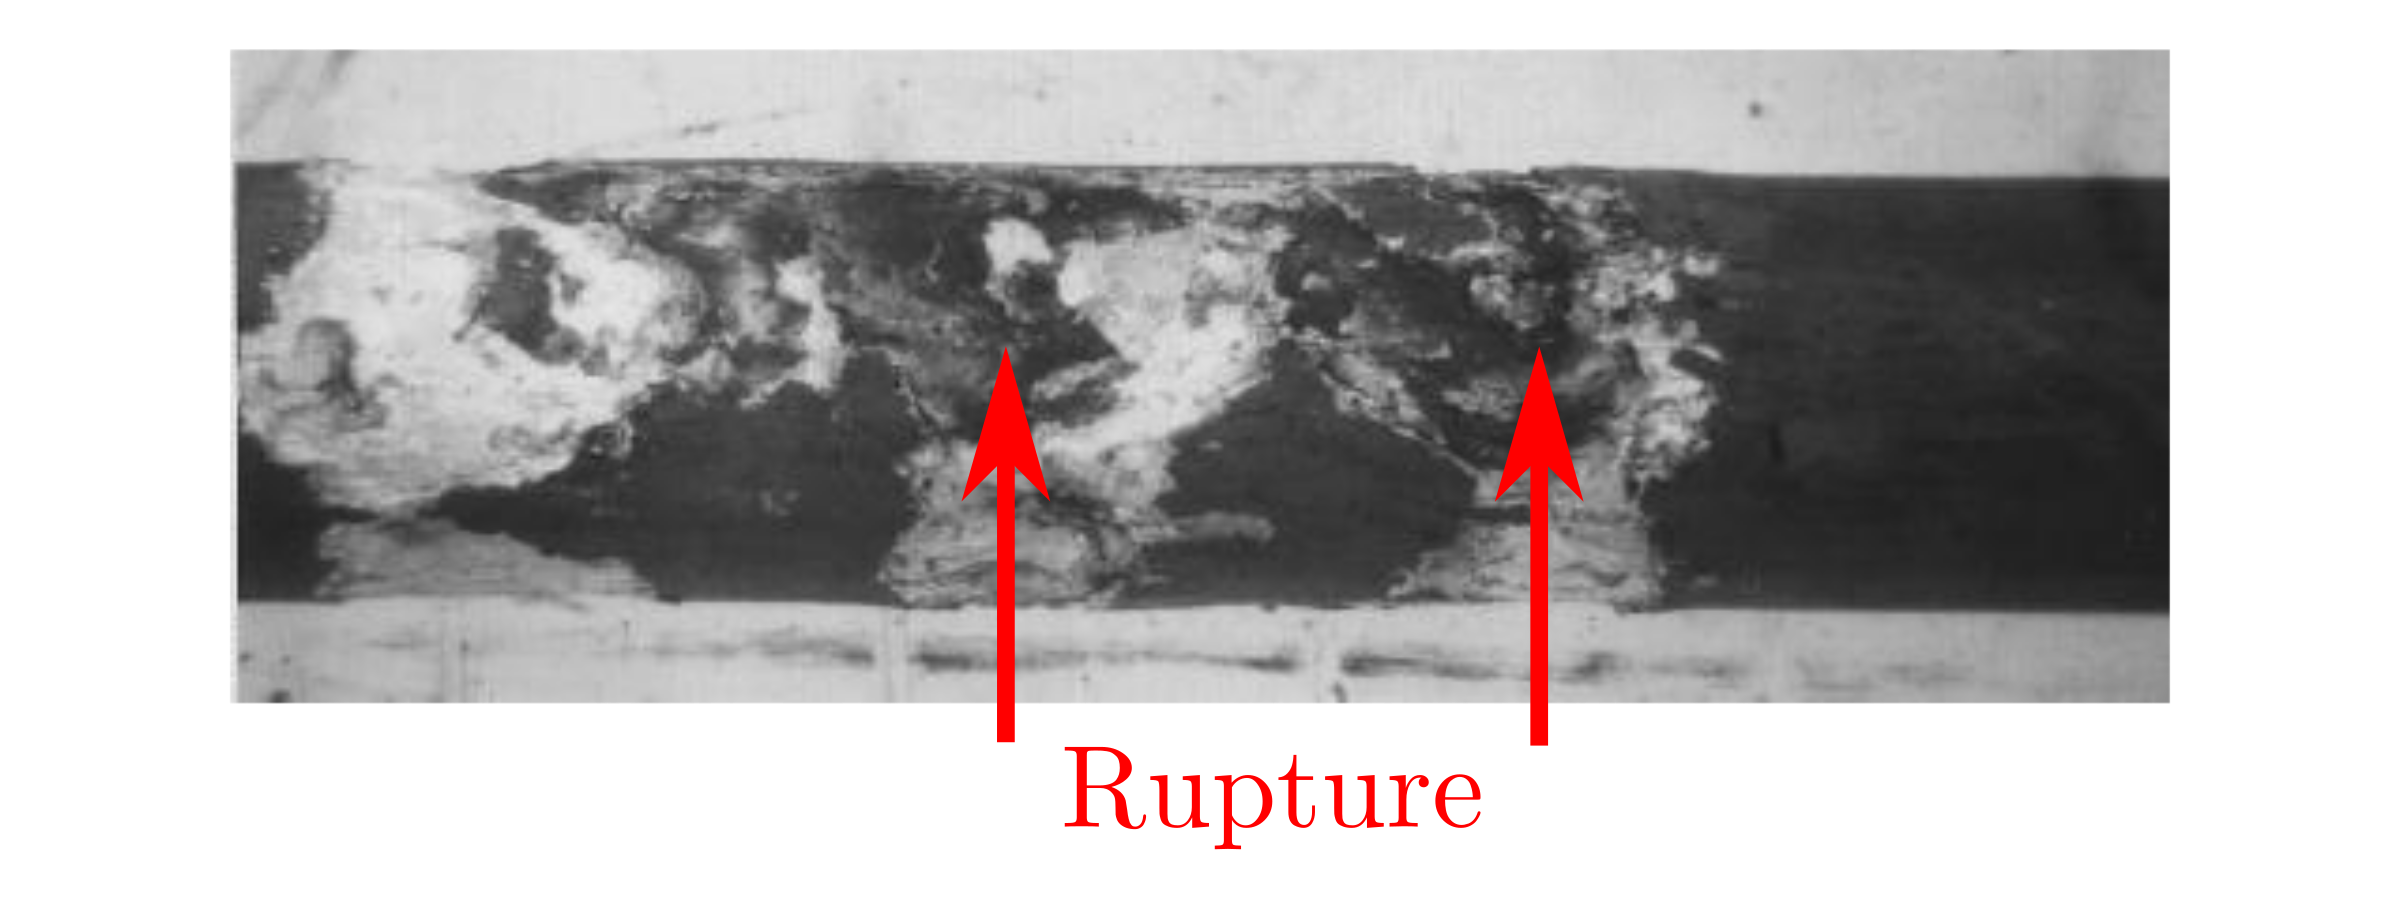
\includegraphics[width=0.6\textwidth]{rod_failure.png}
        \caption[Photographie illustrant la rupture d'une gaine de confinement dans le réacteur KKL]
        {Photographie illustrant la rupture d'une gaine de confinement dans le réacteur KKL \citep{Edsinger2004}.} 
        \label{fig:fuel_rod_failure_KKL} 
     \end{figure}


Des suivis de l'évolution de l'épaisseur de zircone sur les gaines sont effectués pendant la durée de mise en service de
ces dernières. Dans le cas de l'incident du réacteur KKL, les valeurs d'épaisseur de zircone ont été mesurées et celles-ci
ont été confrontées aux valeurs d'épaisseur de zircone obtenus lorsque le phénomène de Shadow Corrosion est absent comme
illustré sur la figure \ref{fig:KKL_shadow_values}. Il semble que le phénomène de Shadow Corrosion est apparu dès la
première année de mise en service avec une augmentation très rapide de l'épaisseur suivie par une période de
stabilisation. Une nouvelle augmentation forte de l'épaisseur de zircone, après trois ans de service, a mené à l'oxydation
totale de la gaine.

La figure \ref{fig:KKL_shadow_digitalization} a été obtenue à partir des données numérisées de la 
figure \ref{fig:KKL_shadow_values}, en calculant les densités de courant équivalentes à partir de l'équation
\ref{eq:th_to_j}. Il est clair que le peu de points disponibles rend cette estimation de la densité de courant très 
approximative. Cependant, elle permet de comparer les ordres de grandeur mis en jeu dans le cas
d'une cinétique d'oxydation classique et d'une cinétique d'oxydation de type Shadow Corrosion. 

    \begin{figure}[H] 
        \centering 
        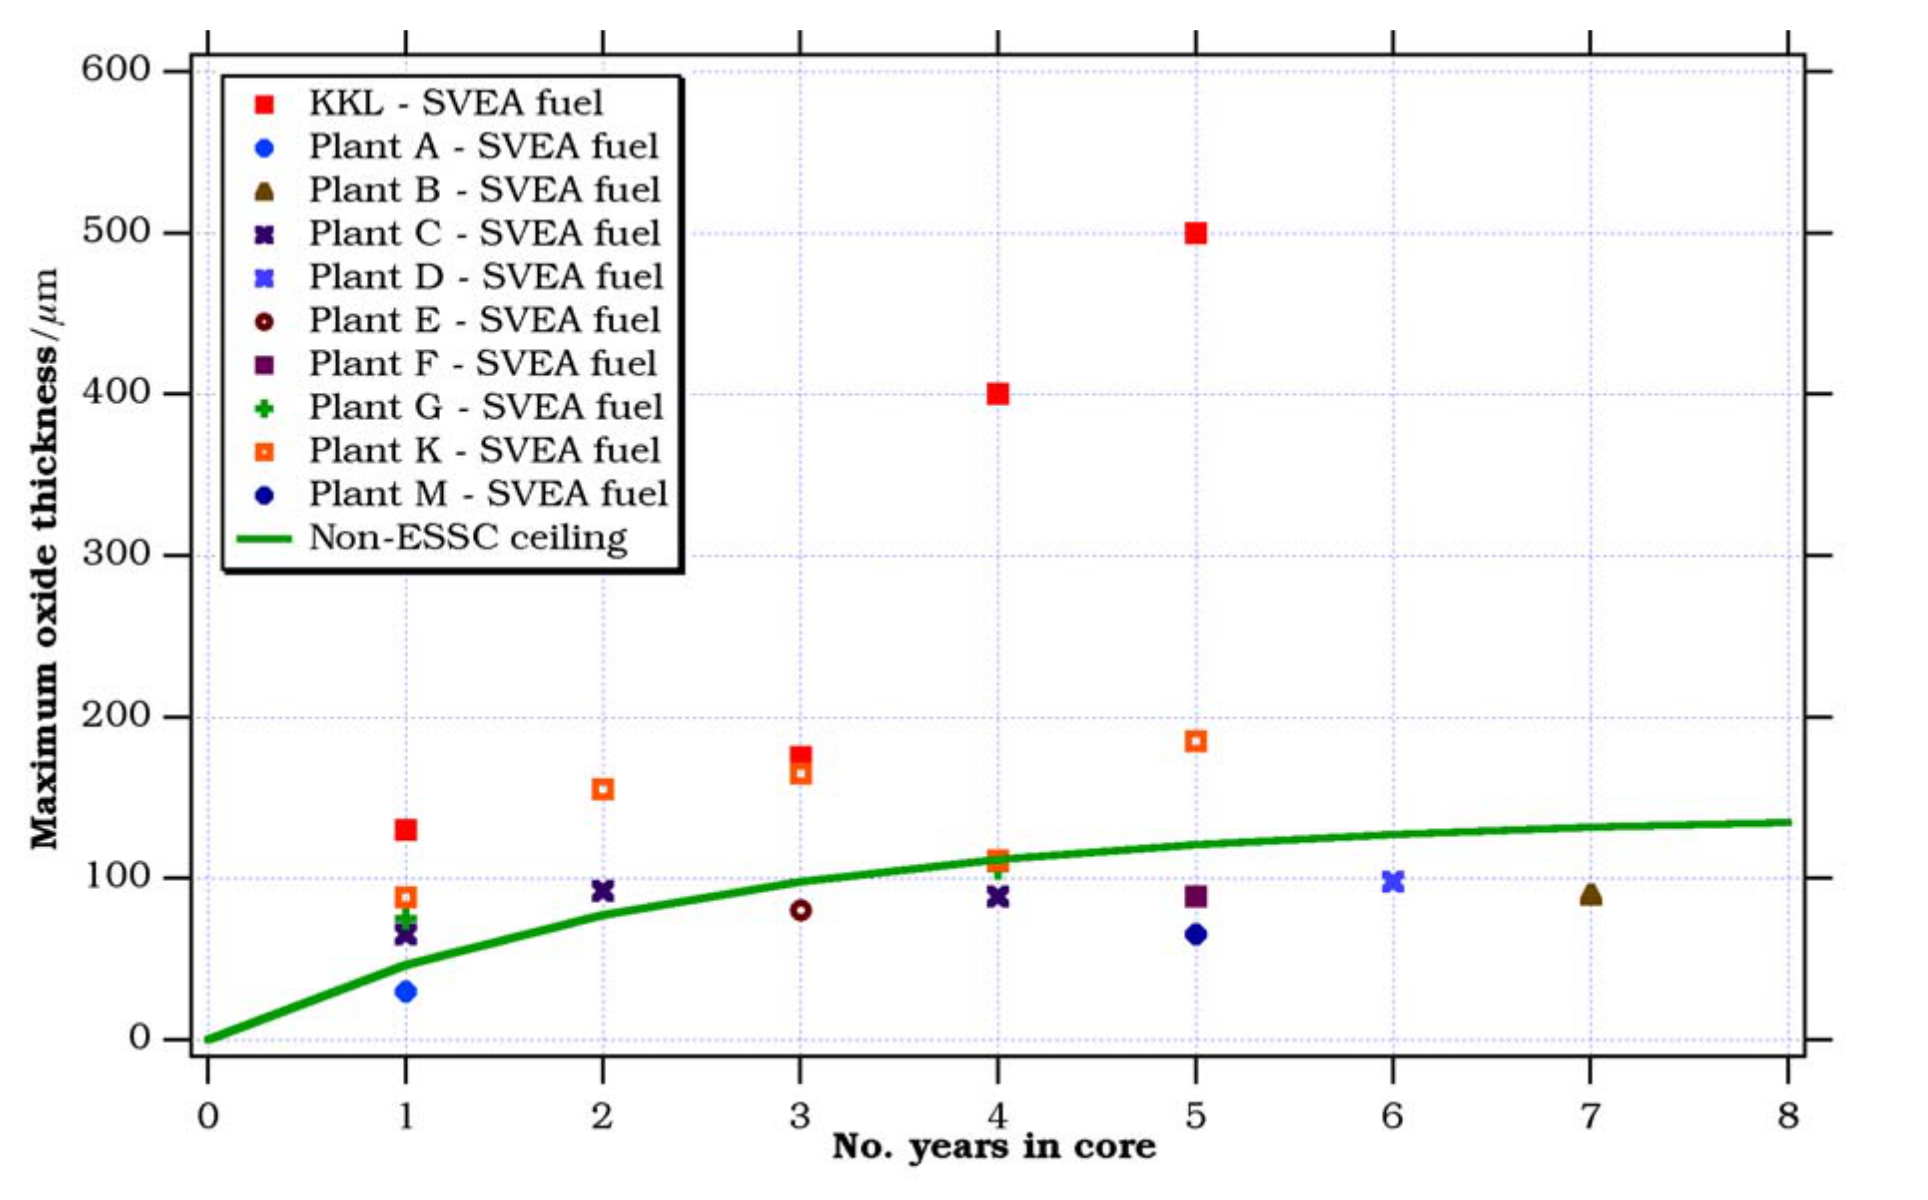
\includegraphics[width=0.65\textwidth]{Edsinger_2004-Fig_2_15.png}
        \caption[Evolution de l'épaisseur de la couche de zircone formée sur les gaines en fonction du temps d'exposition en réacteur
        dans le cas d'une corrosion classique et dans le cas de Shadow Corrosion.]
        {Evolution de l'épaisseur de zircone formée sur les gaines en fonction du temps d'exposition en réacteur
        dans le cas d'une corrosion classique et dans le cas de Shadow Corrosion \citep{Edsinger2004}.} 
        \label{fig:KKL_shadow_values} 
     \end{figure}  

     \begin{figure}[H]
         \centering
            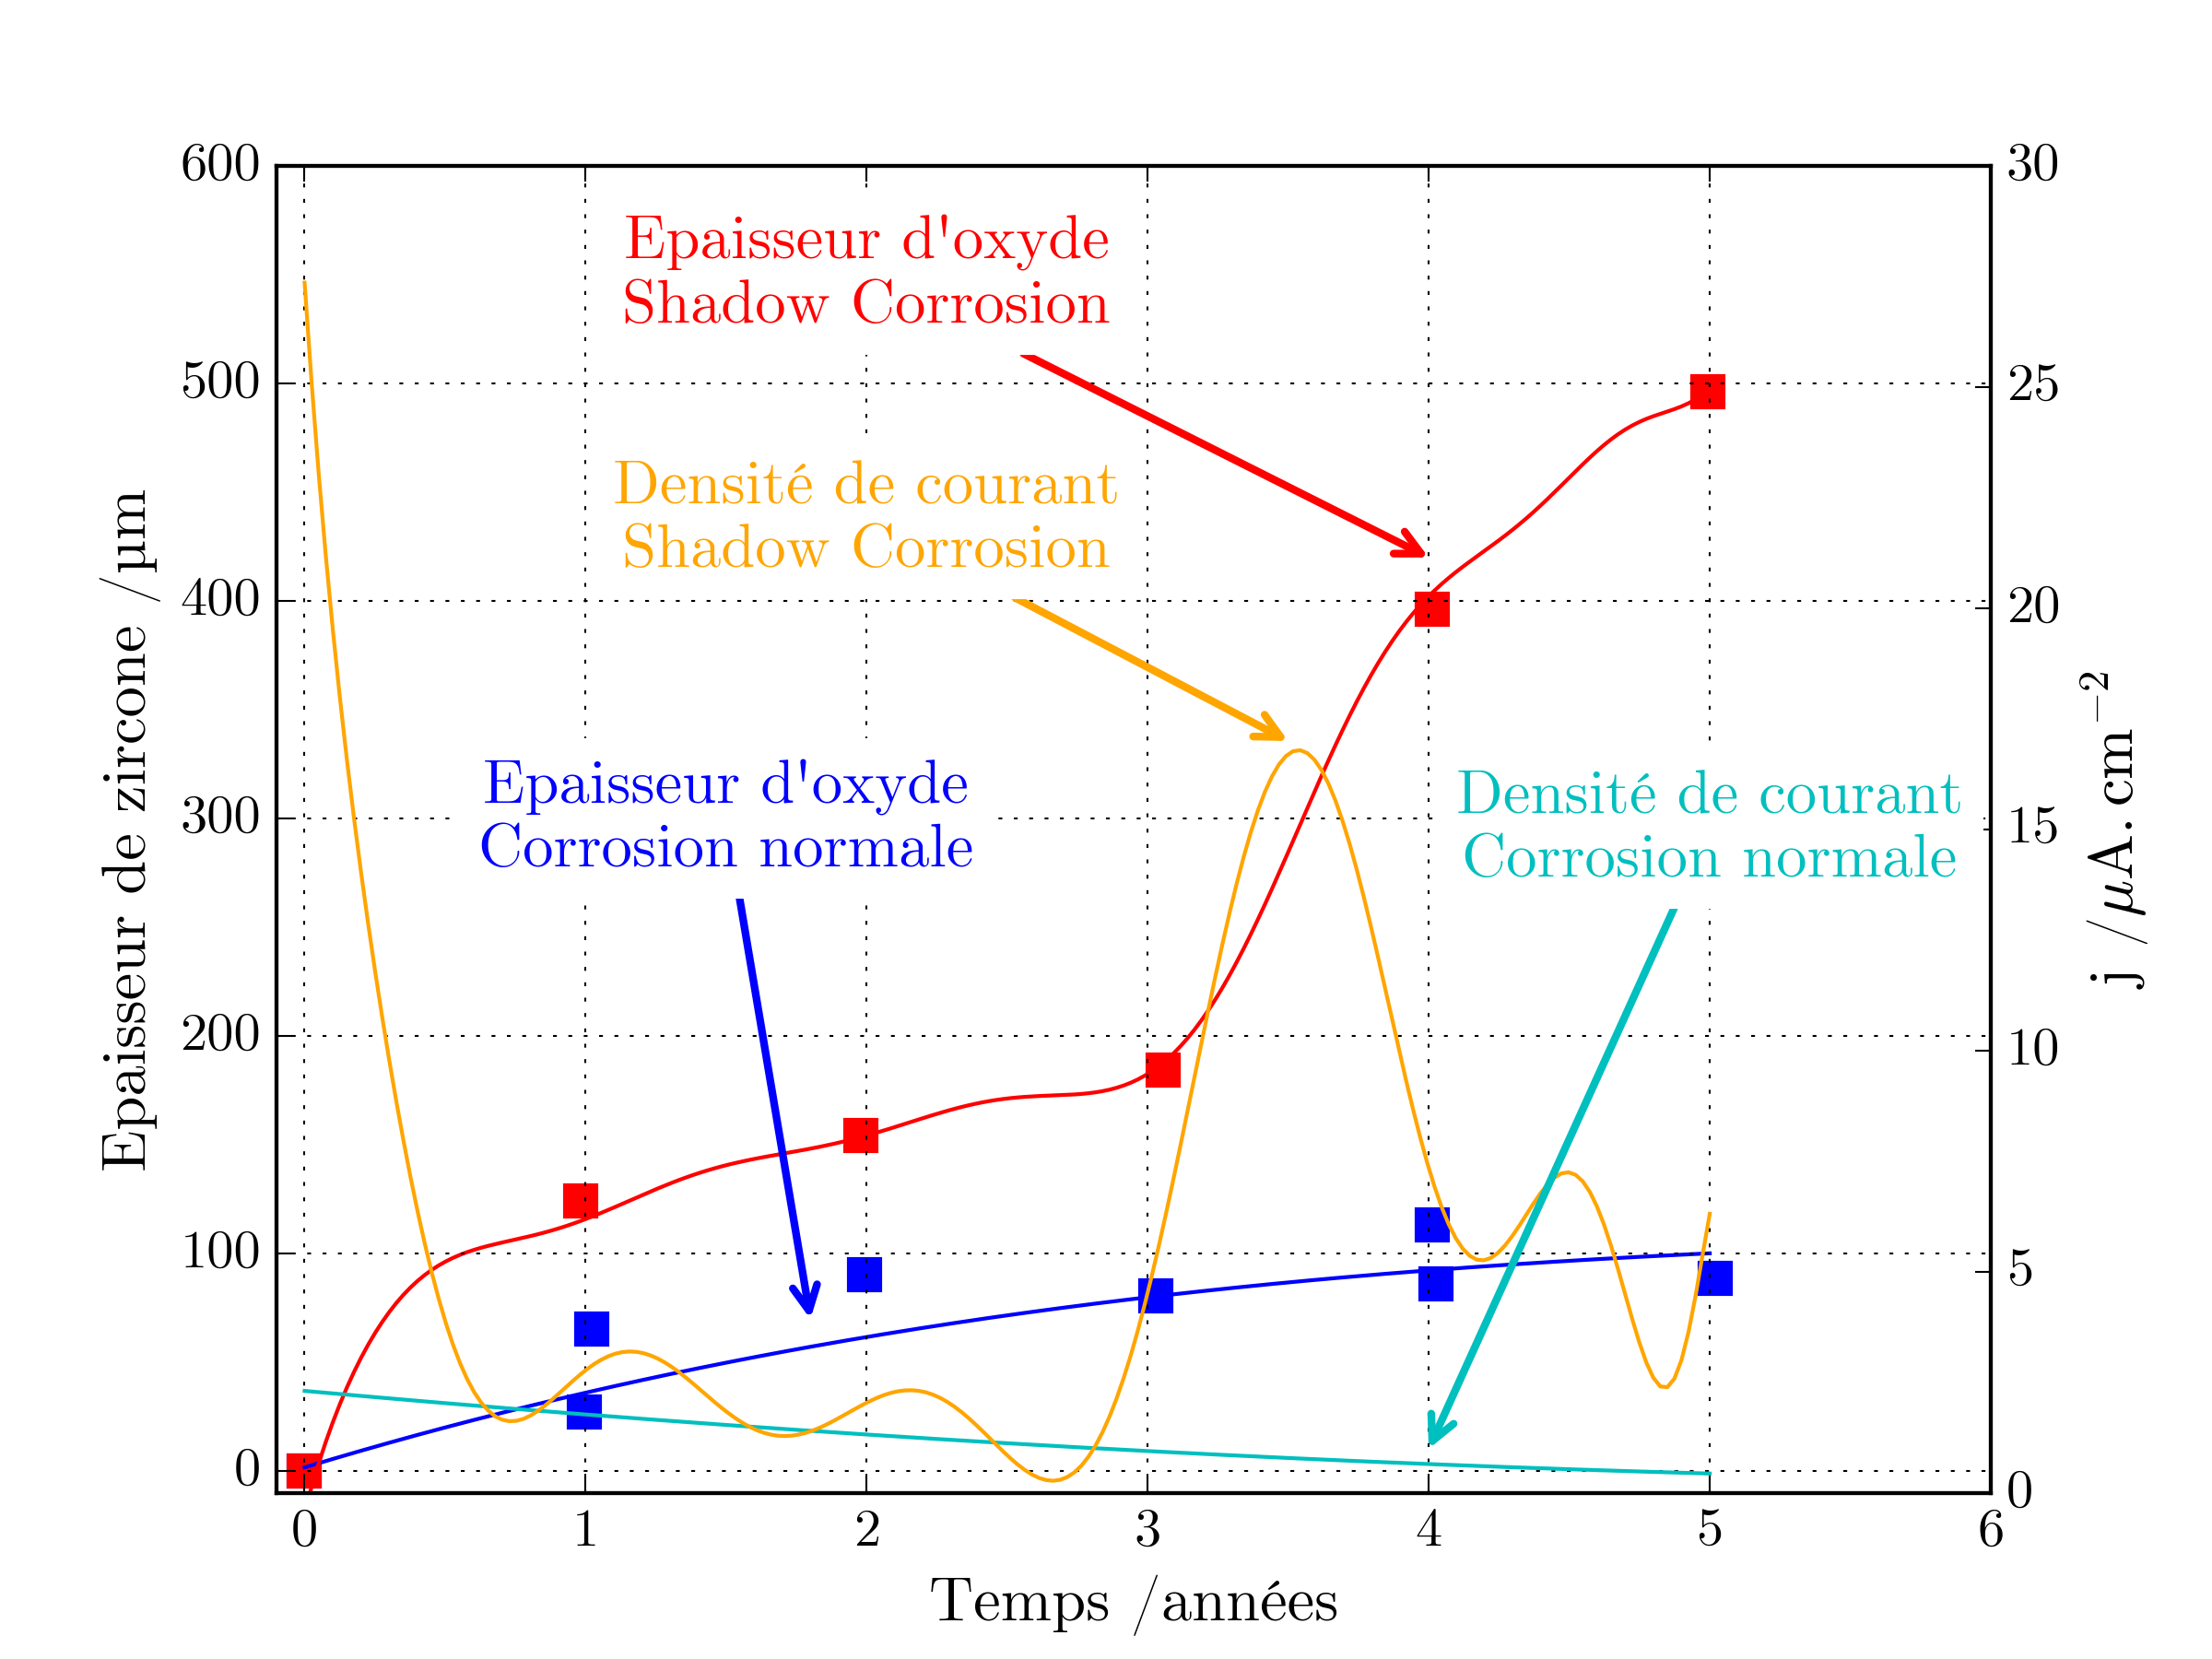
\includegraphics[width=0.65\textwidth]{Bischoff_2012_Fig2-Plot.png}
            \caption{Densité de courant équivalentes calculées selon l'équation \ref{eq:th_to_j} à partir des données
            numérisées de la figure \ref{fig:KKL_shadow_values}.} 
            \label{fig:KKL_shadow_digitalization} 
    \end{figure} 
    
Dans le cas d'une corrosion classique, la densité de courant diminue constamment à partir de valeurs initiales
 de quelques \si{\micro\ampere\per\square\centi\meter} 
jusqu'à des valeurs finales de quelques dizaines de \si{\nano\ampere\per\square\centi\meter}.
En Shadow Corrosion on mesure une densité de courant initiale de quelques dizaines de 
\si{\micro\ampere\per\square\centi\meter}. Pendant la période de stabilisation, celle-ci reprend à des valeurs proches
des valeurs observées dans le cas d'une corrosion classique.
Après trois ans de fonctionnement, la densité de courant augmente à nouveau pour atteindre des valeurs voisines de
\SI{10}{\micro\ampere\per\square\centi\meter}. Cette analyse, certes très approximative, permet à minima de constater que la
densité de courant liée à la Shadow Corrosion est environ dix fois plus élevée que dans le cas d'une corrosion classique.


%%%%%%%%%%%%%%%%%%%%%%%%%%%%%%%%%%%%%%%%%%%%%%%%%%%%%%%%%%%%%%%%%%%%%%%%%%%%%%%%%%%%%
%%%%%%%%%%%%%%%%%%%%%%%%%%%%%%%%%%%%%%%%%%%%%%%%%%%%%%%%%%%%%%%%%%%%%%%%%%%%%%%%%%%%%
\section{Etudes expérimentales de la Shadow Corrosion en réacteur test}\label{sec:in_pile_reactor}

    A la suite de l’incident du réacteur KKL, Westinghouse a lancé trois séries de
    tests expérimentaux dans des réacteurs de recherche afin
    d’étudier le phénomène de Shadow Corrosion. Ces réacteurs de recherche
    permettent de simuler les conditions de fonctionnement d’un REB
    en termes de pression, de température, de flux de neutron et de chimie de
    l’eau. Les résultats issus de ces expériences ont permis de lister les
    paramètres qui semblaient avoir un impact fort sur le phénomène de Shadow Corrosion.

    Les études expérimentales ont été menées dans trois réacteurs de recherche différents :
    le réacteur de Studsvik R2 en Suède \citep{Nystrand1999}, le réacteur MITR-II
    aux Etats-Unis \cite{Chatelain2000} et le réacteur de Halden en Norvège
    \cite{Andersson2002}. La principale donnée de sortie était l’épaisseur de la
    couche de zircone qui s’est formée sur la gaine en Zircaloy-2 mesurée par observation métallographique ou par mesure
    des courants de Foucault.

    \subsection{Essais effectués dans le réacteur de Studvik (Suède)}\label{subsec:studvik}

	\subsubsection{Conditions expérimentales des essais}
        L’objectif de ce premier test était de vérifier si le phénomène de Shadow
        Corrosion peut être observé sur des gaines de confinement en Zircaloy-2
        placés dans une grille de maintien en alliage de nickel X750 après une
        courte période d’exposition dans le coeur du réacteur test. Les gaines de
        Zircaloy-2, en contact avec les grilles de maintien, étaient placées en parallèle dans le
        coeur et hors du coeur du réacteur pendant 5 semaines avec une chimie
        déficiente en fer comme dans le cas de l’incident du réacteur KKL.
        Différents traitement de surface ont été testés sur les gaines de Zircaloy-2 dont  
        quatre ont été pré-oxydés jusqu'à une épaisseur de zircone de
        \SI{1}{\micro\meter} et deux jusqu'à une épaisseur de
        \SI{2}{\micro\meter}.
	
	\subsubsection{Résultats des essais}
        Le même phénomène que dans les réacteurs commerciaux a été observé
        c’est-à-dire que les échantillons placés dans le coeur du réacteur présentaient
        une couche de zircone de \SI{10}{\micro\meter} alors que les échantillons
        placés hors du coeur présentaient une couche de zircone de \SI{1}{\micro\meter}. L'augmentation d'épaisseur de la couche
        de zircone n'a été observée qu'au point de contact et aucune surépaisseur n'a été observée dans la zone autour
        du point de contact grille-gaine.
        Il n’y a pas d’effet notable du traitement de surface. 

        La présence d’irradiation
        semble donc être une condition nécessaire pour reproduire le
        phénomène de Shadow Corrosion. Cependant, l’absence de couplage entre la
        gaine et la grille est une condition expérimentale qui n'a pas été étudiée.


    \subsection{Essais effectués dans le réacteur du MIT (USA)}\label{subsec:MIT}

    \subsubsection{Conditions expérimentales des essais}
        L’objectif premier de ce test était d’étudier l’impact des matériaux de
        contre-électrode, c’est-à-dire les matériaux des grilles de maintien, sur le
        phénomène de la Shadow Corrosion. La durée de l'exposition était d'environ 7 semaines.
        Quatre matériaux ont été testés: l'alliage de
        nickel X750, le platine, l’alliage Nitronic 32 et l'alliage Zircaloy-2 qui est
        également le matériau de la gaine. L’alliage Nitronic 32 est alliage austénitique
        de fer contenant 12 \% en masse de manganèse qui est un émetteur de radiation $\beta$
        lorsqu’il est activé. Les échantillons étaient placés dans deux types de modules :
        module \emph{sans contact} et module \emph{avec contact}, représentés en figures
        \ref{fig:Modules_MIT_Test} et \ref{fig:Modules_MIT_Test_schematics}.

        \begin{figure}[H] 
            \centering 
            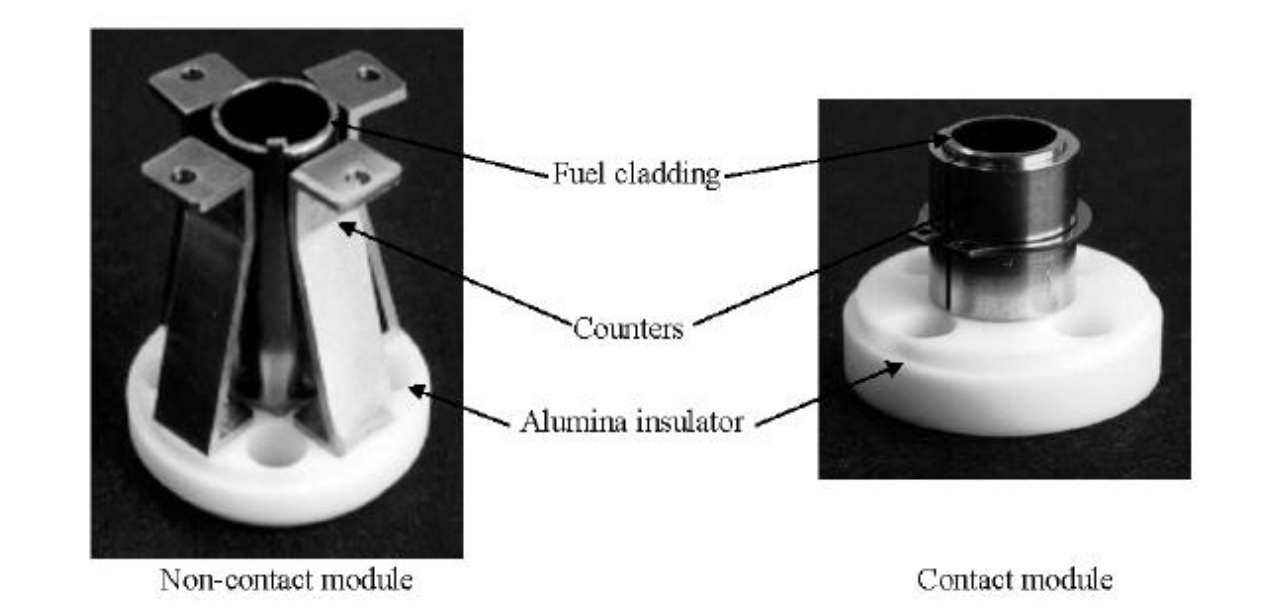
\includegraphics[width=0.65\textwidth]{Bischoff_2012_Fig8.png} 
            \caption[Photographies des modules testés dans le réacteur MITR-II.]
            {Photographies des modules testés dans le réacteur MITR-II \citep{Chatelain2000}.} 
            \label{fig:Modules_MIT_Test} 
        \end{figure}
        
        \begin{figure}[H] 
            \centering 
            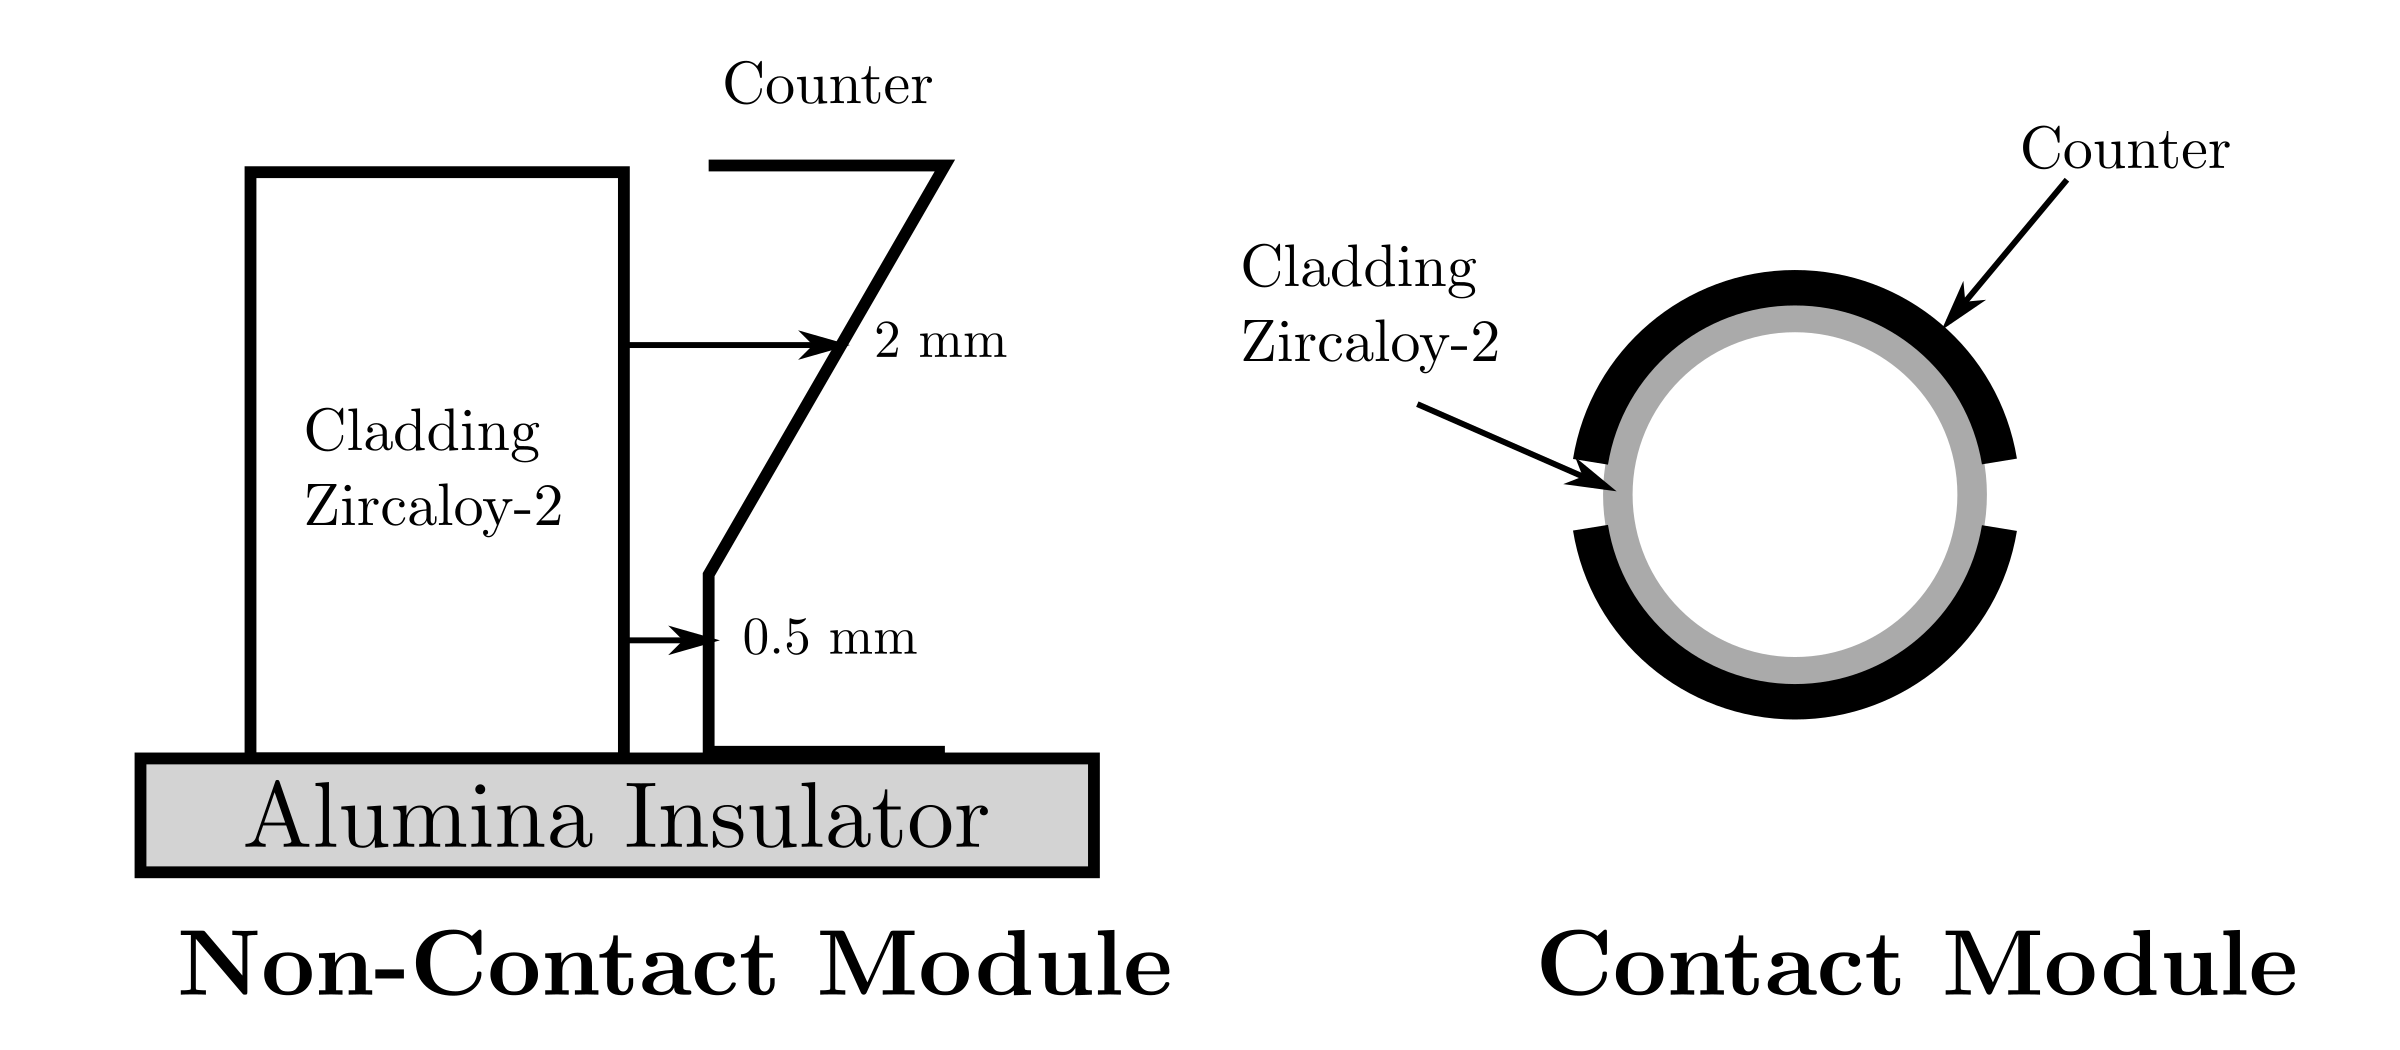
\includegraphics[width=0.65\textwidth]{Chatelain_2000-Modules-Both-Redrawn.png} 
            \caption[Représentation schématique des modules testés dans le réacteur MITR-II.]
            {Représentation schématique des modules testés dans le réacteur MITR-II \citep{Chatelain2000}.} 
            \label{fig:Modules_MIT_Test_schematics} 
        \end{figure}

        Les modules avec contact étaient constitués d’une gaine de Zircaloy-2 avec deux
        moitiés de tube en guise de contre-électrodes, ces dernières étant mises en contact
        avec la gaine et maintenues par un anneau en acier inoxydable. L’ensemble était
        placé sur un isolant en alumine. Les modules sans contact sont réalisés en
        isolant une gaine de Zircaloy-2 avec de l’alumine par rapport aux quatre contre-électrodes
        qui font face à la gaine. La forme des contre-électrodes permettait de
        contrôler leur distance (entre \SI{0.5}{\milli\meter} et \SI{2}{\milli\meter}) à la gaine en Zircaloy-2.

        La chimie d’un REB était reproduite dans le réacteur et le flux d’eau formait une boucle dans le
        réacteur comme illustré sur la figure \ref{fig:MITRII_reactor_schematics}. Des
        échantillons étaient placés dans le coeur, et hors du coeur du réacteur à environ
        \SI{60}{\milli\meter} en aval. Les échantillons ont été exposés pendant une période de 7 semaines, la dose
        de rayonnement gamma était environ deux ordres de grandeur inférieure hors du coeur
        par rapport au coeur alors que la dose de rayonnement neutronique était environ inférieure de cinq ordres de
        grandeurs.

	\begin{figure}[H] 
 		\centering 
 		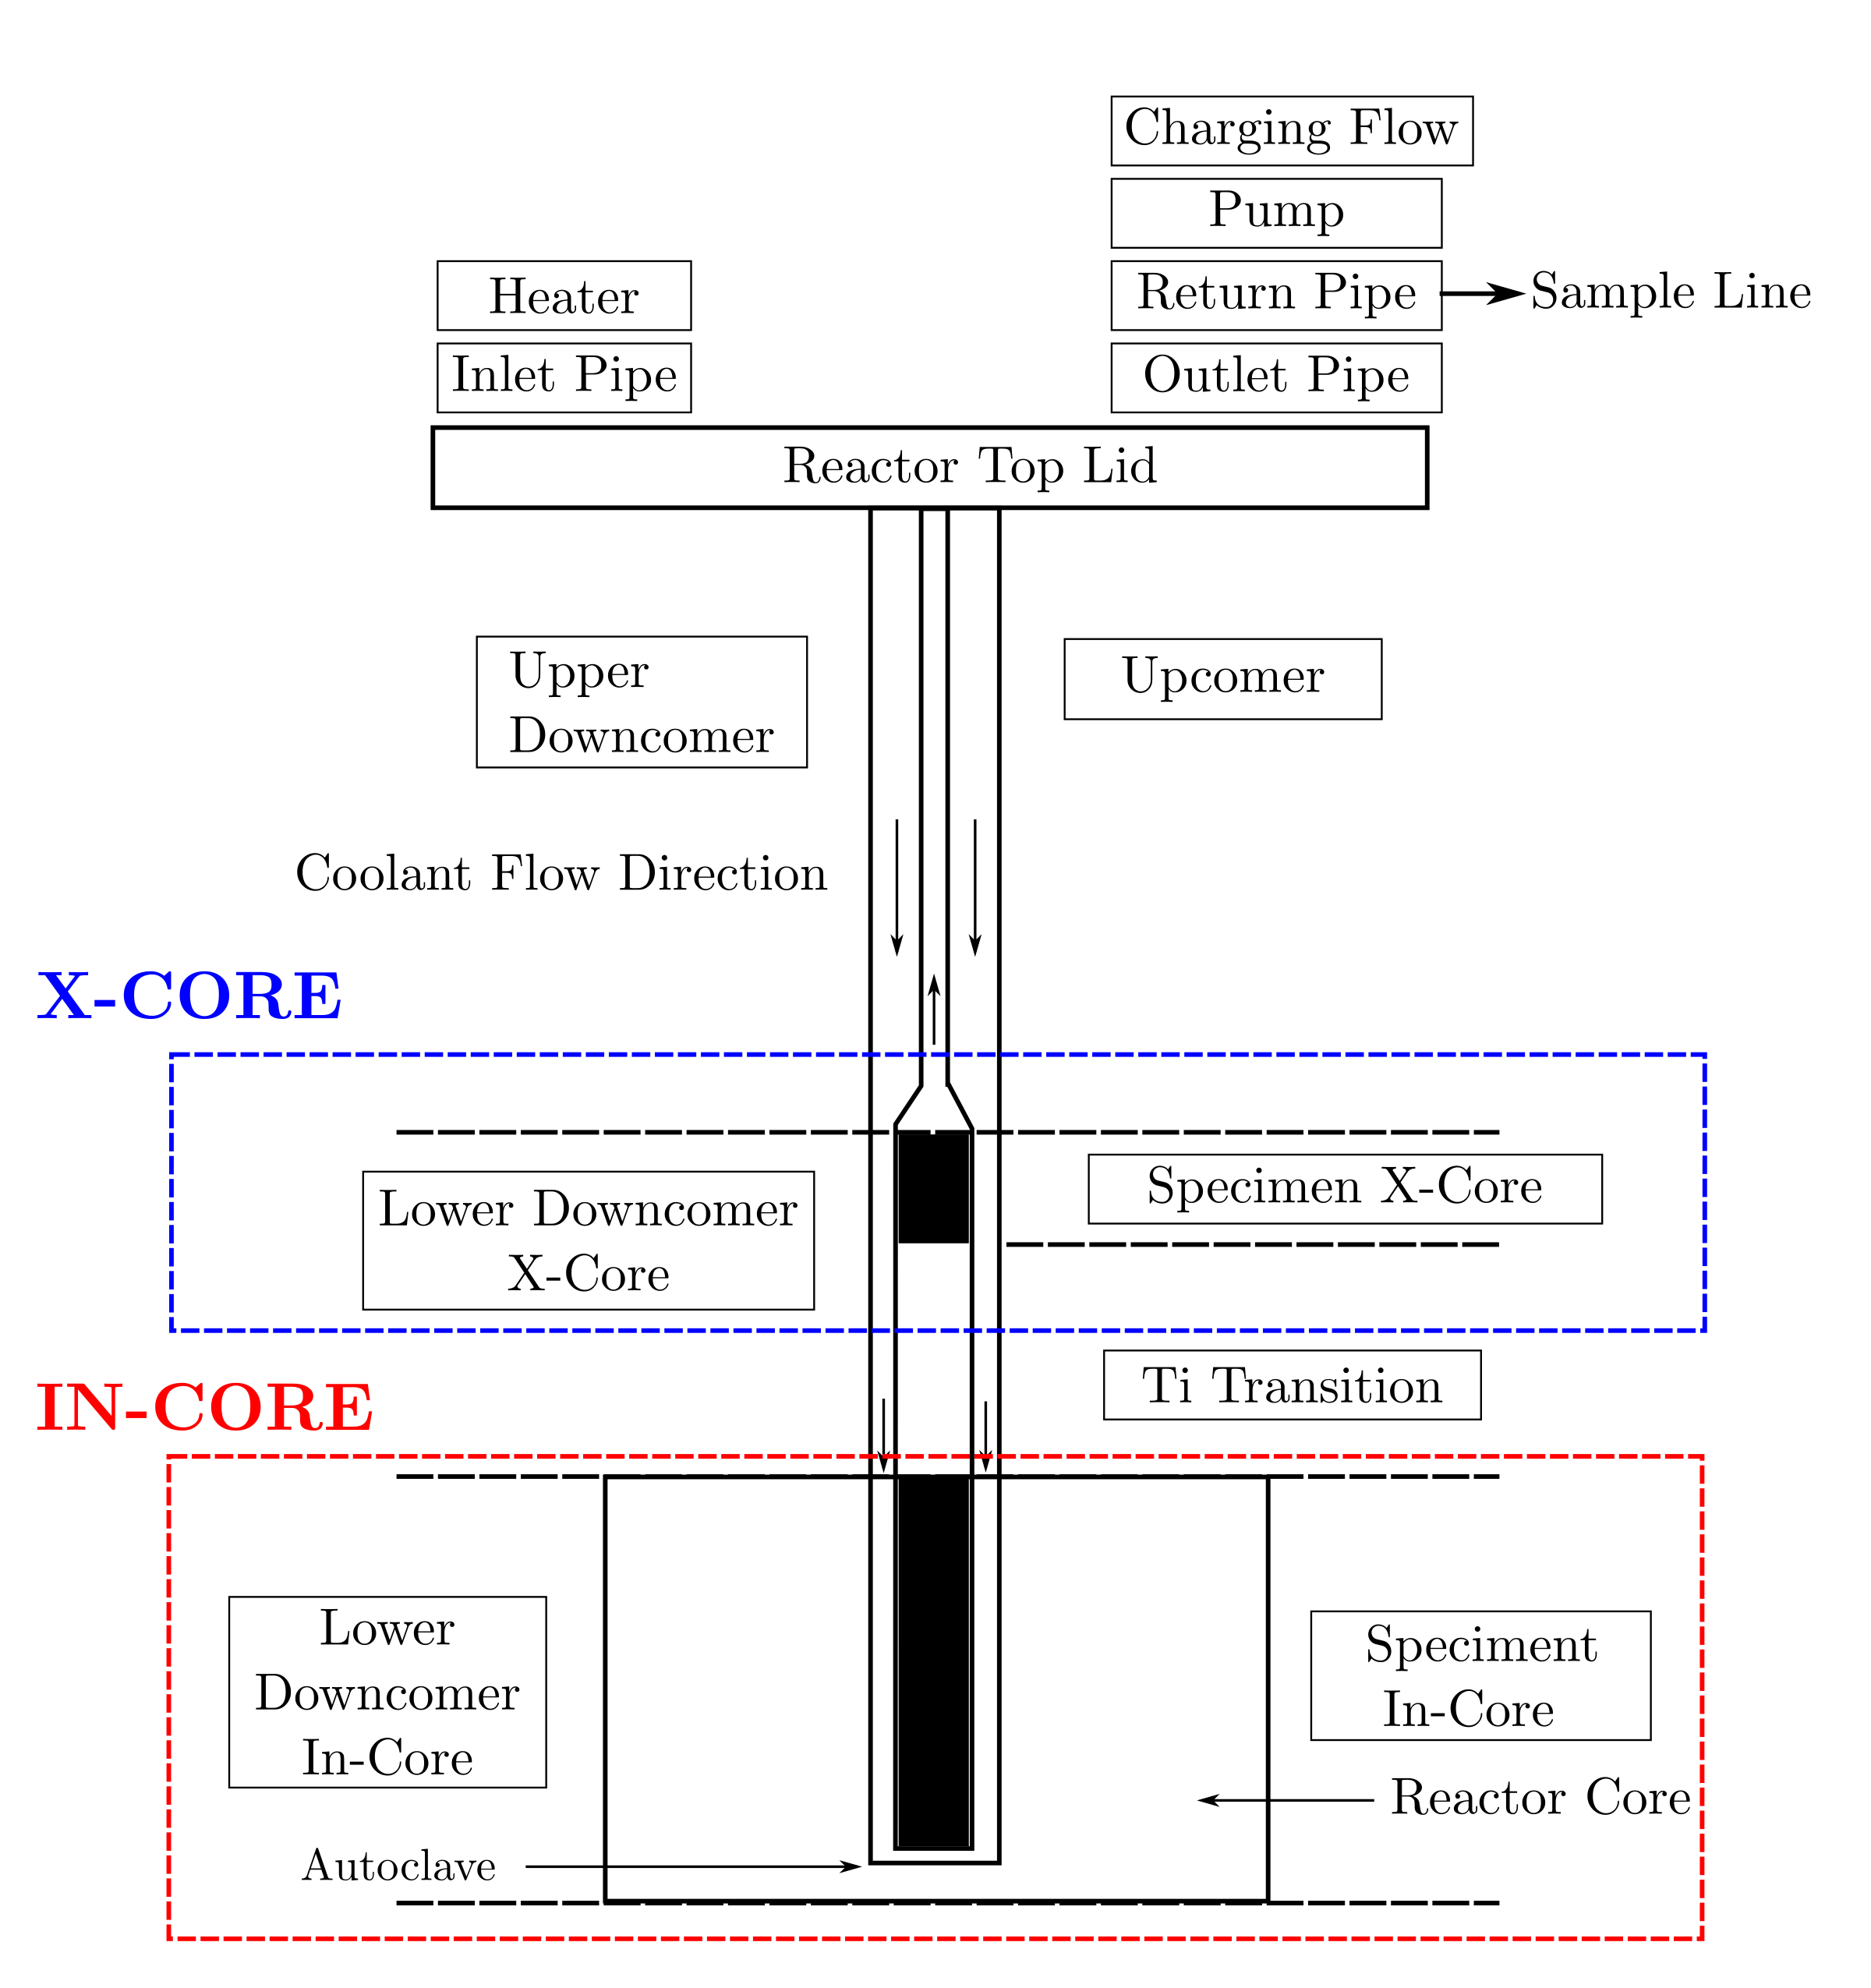
\includegraphics[width=\textwidth]{Chatelain_2000-InCore_ExCore_Locations-2.png} 
        \caption[Représentation schématique du réacteur test MITR-II.]
        {Représentation schématique du réacteur test MITR-II \citep{Chatelain2000}.} 
 		\label{fig:MITRII_reactor_schematics} 
 	\end{figure}
	
	\subsubsection{Résultats des essais}
        Dans le cas des modules sans contact, le phénomène de Shadow Corrosion n'a été
        observé qu'avec l’alliage de nickel X750 et le platine, quelles que
        soient les configurations expérimentales comme illustré en figure
        \ref{fig:oxide_thickness_vs_counter_material_non_contact_module}. Le
        phénomène de Shadow Corrosion apparaissant deux fois moins prononcé sur les
        échantillons hors du coeur. Par ailleurs, l’épaisseur de zircone était inversement
        proportionnelle à la distance entre la gaine et la contre-électrode
        (\ref{fig:oxide_thickness_vs_distance_non_contact_module}), l'ampleur du phénomène
        de Shadow Corrosion était rapidement atténué au-delà de
        \SI{1}{\milli\meter}. Il faut cependant souligner que l’alumine n’est pas un
        isolant parfait lorsqu'elle est irradiée \citep{Shikama1994} et
        que les modules dits sans contact ne peuvent donc probablement pas être réellement considérés en tant que
        tels.

        \begin{figure}[H]
            \centering
            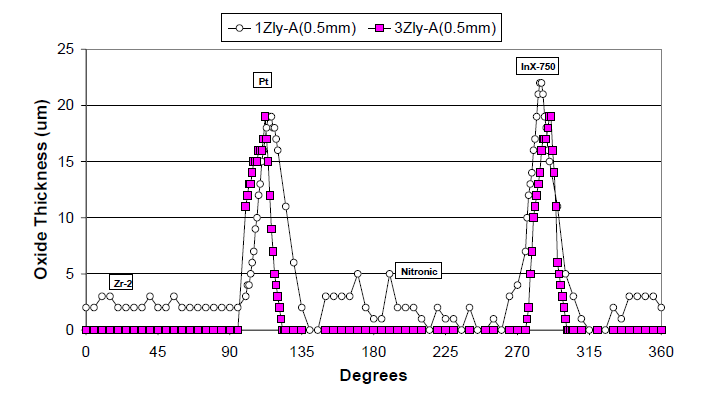
\includegraphics[width=0.65\textwidth]{Bischoff_2012_Fig9.png} 
            \caption[Epaisseurs de zircone mesurées sur le module sans contact en fonction des quatre types matériaux de
            contre-électrode pour une distance gaine--contre-électrode de \SI{0.5}{\milli\meter}.]
            {Epaisseurs de zircone mesurées sur le module sans contact en fonction des quatre types matériaux de
            contre-électrode pour une distance de \SI{0.5}{\milli\meter} \citep{Chatelain2000}.} 
            \label{fig:oxide_thickness_vs_counter_material_non_contact_module} 
        \end{figure}

        \begin{figure}[H] 
            \centering
            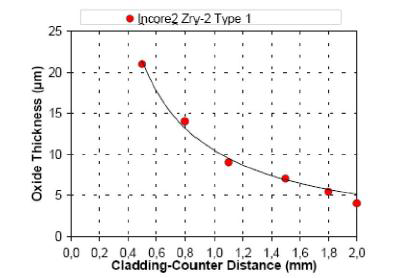
\includegraphics[width=0.65\textwidth]{Bischoff_2012_Fig10.png} 
            \caption[Epaisseurs de zircone mesurées en fonction de la distance pour le couple Zircaloy-2/X750.]
            {Epaisseurs de zircone mesurées en fonction de la distance gaine--contre-électrode pour le couple Zircaloy-2/X750 \citep{Chatelain2000}.}
            \label{fig:oxide_thickness_vs_distance_non_contact_module} 
        \end{figure}

        
        Sur les gaines des modules avec contact, il n a pas été observé de corrosion aggravée
        sur la surface située sous la contre-électrode. Cependant, une surépaisseur
        d’oxyde est apparue au voisinage de l’espacement entre les deux demi-tubes formant la
        contre-électrode, probablement en raison que l’électrolyte peut y accéder
        plus facilement à la surface de la gaine, favorisant ainsi le renouvellement
        de la chimie locale. Malgré une surface de contact élevée entre la gaine et les
        contre-électrodes, les modules avec contact présentent une surépaisseur
        d’oxyde plus faible que les modules sans contact quelle que soit leur position
        dans le réacteur. Tout comme pour les modules sans contact, seuls l’alliage de
        nickel X750 et le platine ont donné lieu au phénomène de Shadow Corrosion.
        
        Le phénomène de Shadow Corrosion apparaît donc avec des matériaux de
        contre-électrode plus nobles que l'alliage Zircaloy-2 tels que l’alliage de nickel X750 et le platine.
        La présence d'une irradiation et les doses de radiations sont des paramètres importants pour l'apparition de la
        Shadow Corrosion.
        La distance grille--gaine est
        également un paramètre important mais l’accès de l’électrolyte à la surface de
        la gaine et de la contre-électrode est tout aussi important. La circulation du
        fluide caloporteur, c’est-à-dire l’électrolyte, permet probablement de renouveler la
        chimie locale et ainsi de favoriser l'apparition de la Shadow Corrosion.

        
%        \citet{Treeman2005} a réalisée des essais supplémentaires dans ce même réacteur afin de quantifier les densités
%        de courants de couplage mis en jeu lorsque l'alliage Zircaloy-2 est en contact avec du Pt ou l'alliage de nickel X750. 
%        L'étude a été mené sur environ 50 jours avec des phases d'interruption. La figure \ref{fig:treeman_jgal}
%        présente les résultats obtenus retracé en fonction de la durée d'exposition afin de mieux visualiser les phases
%        à haute température ainsi que les phases à forte dose d'irradiation. 

%        Les résultats obtenus sont intéressants puisqu'ils mettent en avant l'importance de la température. A 20
%        d'exposition, la puissance du coeur est au maximum alors la température est à environ \SI{60}{\degreeCelsius}.
%        La densité de courant de couplage se situe à \SI{\sim 0.5}{\micro\ampere\per\square\centi\meter}. En maintenant,
%        la puissance constante et en augmentant la température à \SI{250}{\degreeCelsius}, la densité de courant de
%        couplage augmente brutalement jusqu'à \SI{\sim 10}{\micro\ampere\per\square\centi\meter}. Ce résultat
%        expérimental confirme bien le lien entre le transport ionique et le transport électronique.

%        \begin{figure}[!htb]
%            \centering
%            \includegraphics[width=0.45\textwidth]{Treeman_2005-Galvanic_Currents.pdf}
%            \caption[Résultats expérimentaux obtenus par Treeman et al. retracés en fonction du temps d'exposition.]
%            {Résultats expérimentaux obtenus par \citet{Treeman2005} retracés en fonction du temps d'exposition.
%            a) Evolution de la température. 
%            b) Evolution des courants de couplage. 
%            c) Evolution de la puissance du coeur.}
%        \end{figure}

        


    \subsection{Essais effectués dans le réacteur de Halden (Norvège)}\label{subsec:halden}

    \subsubsection{Conditions expérimentales des essais}
        Les objectifs de ce test était d'évaluer l’impact du flux
        neutronique, du flux de rayonnement gamma, des traitements thermiques, de la
        composition chimique des gaines de confinement et des matériaux de
        contre-électrode sur le phénomène de Shadow Corrosion dans le cas d'une exposition de longue durée. Un test
        complémentaire était axé sur l’impact de traitements de surfaces des
        gaines.
	
        Le matériau de la gaine était toujours l’alliage de Zircaloy-2. Plusieurs
        matériaux de contre-électrodes ont été testés: l’alliage de nickel X750, un alliage de
        zirconium ZrSnCrNi et un alliage de zirconium ZrSnFe dépourvu d’éléments
        d’alliage plus nobles tels que le Cr et le Ni. Les gaines et les
        contre-électrodes, en contact, ont été exposées dans le coeur du réacteur pendant
        une durée de 289 jours. 

	
	\subsubsection{Résultats des essais}
        Les résultats de ces essais ont montré que le phénomène de Shadow Corrosion est
        plus prononcé dans les régions où les flux de neutrons et de rayonnement
        gamma sont plus importants. Tout comme lors des tests dans le réacteur de Studvik, 
        le phénomène de Shadow Corrosion a été
        observée au point de contact mais il a, ici également, été observé dans la zone autour du point de contact.
        Il a été noté qu'une taille des précipités importante semblait diminuer
        la résistance à la Shadow Corrosion. Cependant, une augmentation plus
        modérée de la taille des précipités, obtenue en modifiant le traitement thermique ou la quantité
        d’éléments d’alliage, ne semblait avoir aucun effet.
	
        Le phénomène de Shadow Corrosion a été observé sur les gaines de Zircaloy-2 situées
        en face des contre-électrodes en alliage de nickel X750 et en alliage de
        zirconium ZrSnFeCrNi, avec une épaisseur de zircone mesurée deux fois moins
        importante avec l’alliage ZrSnFeCrNi. Dans le cas du couple Zy2/ZrSnFe,
        le phénomène de Shadow Corrosion est apparu sur l'alliage ZrSnFe et non pas sur l'alliage Zy2.

        Enfin, les gaines décapées puis pré-oxydées ainsi que les gaines simplement pré-oxydées
        ont montré une meilleure résistance à la Shadow Corrosion.


%%%%%%%%%%%%%%%%%%%%%%%%%%%%%%%%%%%%%%%%%%%%%%%%%%%%%%%%%%%%%%%%%%%%%%%%%%%%%%%%%%%%%
%%%%%%%%%%%%%%%%%%%%%%%%%%%%%%%%%%%%%%%%%%%%%%%%%%%%%%%%%%%%%%%%%%%%%%%%%%%%%%%%%%%%%
\section{Mécanismes proposés pour le phénomène de Shadow Corrosion}\label{sec:mechanisms}


    \subsection{Couplage galvanique}\label{subsec:galvanic_coupling}
    A partir des résultats obtenus dans le réacteur MITR-II (\S\ref{subsec:MIT}), \citet{Lysell2004} proposent un 
    mécanisme de couplage galvanique pour la Shadow Corrosion dont une représentation schématique est présentée 
    sur figure~\ref{fig:lysell_mechanism}. La force motrice du couplage galvanique est la différence de potentiel 
    entre la gaine en Zircaloy-2 et la contre-électrode en platine ou en alliage de nickel X750. 
    Le couplage nécessite que les deux matériaux soient en contact électrique ce qui est très certainement le cas puisque 
    l’alumine ne peut être considérée comme un isolant lorsqu’elle irradiée \citep{Shikama1994}. 

     \begin{figure}[H] 
            \centering 
            
\includegraphics[width=0.85\textwidth]{Lysell_2004-Mechanism-1.png}
            \caption[Représentation schématique du mécanisme couplage galvanique: 
            a) représentation schématique du système réel au niveau du contact entre
            le ressort de la grille de maintien et la gaine de confinement, 
            b) représentation schématique sous forme de circuit électrique équivalent du système de couplage.]
            {Représentation schématique du
                mécanisme de couplage galvanique (d'après \citet{Lysell2004}): 
            a) représentation schématique du système réel au niveau du contact entre
            le ressort de la grille de maintien et la gaine de confinement, 
            b) représentation schématique sous forme de circuit électrique équivalent du système de couplage.} 
            \label{fig:lysell_mechanism} 
 	\end{figure}


    Le mécanisme de couplage galvanique proposé par Lysell permet d’expliquer la diminution d’épaisseur de l’oxyde en
    fonction de la distance entre les électrodes car la chute de potentiel dans l’électrolyte augmente avec la distance.
    Les radiations ont pour effet d’accélérer le processus en augmentant la conductivité électronique
    des oxydes qui se forment sur la
    gaine de confinement et sur les grilles de maintien et elles accélèrent le passage du courant dans l'alumine. 
    Mais les effets de la radiolyse de l’eau ne sont pas pris en compte
    dans ce mécanisme.

    Ce mécanisme est aujourd'hui assez largement admis dans la communauté scientifique du nucléaire.
    Il faut tout de même noter que le transport ionique dans la couche de zircone est
    certainement un élément à prendre en compte, car le courant
    galvanique global sera fixé par le transport ionique dans la couche de zircone si ce dernier est limitant par rapport au
    transport électronique.


       
    \subsection{Radiolyse locale}\label{subsec:local_radiolysis}
    \citet{Ramasubramanian2004} a proposé un mécanisme basé sur la radiolyse locale en postulant que le contact
    électrique, nécessaire dans le mécanisme de couplage galvanique, n’est pas assuré. Ramasubramanian base son
    mécanisme sur l’alignement des niveaux d’énergies de la zircone et du platine avec ceux des couples redox issues de
    la radiolyse de l’eau. Le peroxyde d’hydrogène est un élément clé de son mécanisme puisque c’est un des produits
    principaux de la radiolyse de l’eau \citep{Saffre2011}. Selon l'auteur, le même raisonnement peut être appliqué à
    l'alliage de nickel en lieu et place du platine.

    Le peroxyde d’hydrogène peut s’oxyder à la surface du platine, et les produits de l’oxydation vont être réduits sur
    la zircone à la surface de la gaine comme schématisé en figure \ref{fig:ramasubramanian_mechanism}. La réduction à
    la surface de la gaine crée un "appel d’électrons" accélérant ainsi l’oxydation de la gaine. La force motrice de ce
    mécanisme est la différence de potentiel entre la gaine et la contre-électrode qui provoque la migration des ions
    $\rm H^+$ soumis au champ électrique.

    La remarque faite à la fin du paragraphe \ref{subsec:galvanic_coupling} peut être à nouveau
    formulée concernant les travaux de Ramasubramanian.

    \begin{figure}[H] 
 		\centering 
 		
\includegraphics[width=0.75\textwidth]{Ramasubramanian_2004-Mechanism.png}
        \caption[Représentation schématique du mécanisme de radiolyse locale.]
        {Représentation schématique du mécanisme de radiolyse locale (d'après \citet{Ramasubramanian2004}).} 
 		\label{fig:ramasubramanian_mechanism} 
 	\end{figure}

       

	
%%%%%%%%%%%%%%%%%%%%%%%%%%%%%%%%%%%%%%%%%%%%%%%%%%%%%%%%%%%%%%%%%%%%%%%%%%%%%%%%%%%%%
%%%%%%%%%%%%%%%%%%%%%%%%%%%%%%%%%%%%%%%%%%%%%%%%%%%%%%%%%%%%%%%%%%%%%%%%%%%%%%%%%%%%%
\section{Etude expérimentale de la Shadow Corrosion hors réacteur}\label{sec:out_of_pile_experiments}

    Plus récemment, une étude expérimentale hors réacteur a été réalisée par
    \citet{Kim2010}. Les auteurs postulent que la lumière UV est responsable de
    modifications de comportement électrochimique des matériaux alors que les
    rayonnements plus intenses, par exemple les rayonnements $\gamma$, impactent
    principalement les propriétés physiques des matériaux. Effectivement, des rayonnements UV sont
    présents dans le coeur du réacteur à cause du rayonnement de Cherenkov, et, 
    comme mentionné dans le paragraphe \S\ref{subsec:with_irradiation}. \citet{Cox1989} a suggéré que l’effet de l’irradiation
    dans le coeur pouvait éventuellement être simulé avec de la lumière UV à condition que
    son énergie soit supérieure à la largeur de bande interdite de la zircone, soit \SI{5}{\electronvolt} ($\rm \lambda <
    \SI{248}{\nano\meter}$). 

    \subsection{Conditions expérimentales des essais}

    Les principaux alliages testés dans cette étude sont l’alliage Zircaloy-2, l’alliage de nickel X750 et
    l’acier inoxydable 304. Les mesures électrochimiques ont été réalisées dans un autoclave équipé d’une fenêtre en saphir
    monocristallin pour permettre le passage de la lumière et connecté à une boucle de contrôle de la chimie comme illustré 
    en figure \ref{fig:kim_autoclave}. La source lumineuse est une lampe à vapeur de mercure dont le faisceau lumineux est
    guidé jusqu'à la fenêtre de saphir par une
    fibre optique. La lumière émise par cette lampe est intense, et polychromatique avec un spectre allant d'environ 
    \SI{200}{\nano\meter} à l'infrarouge. Dans la suite, l'illumination avec cette lampe sera désignée par illumination
    UV--Visible. 


        \begin{figure}[H] 
            \centering 
            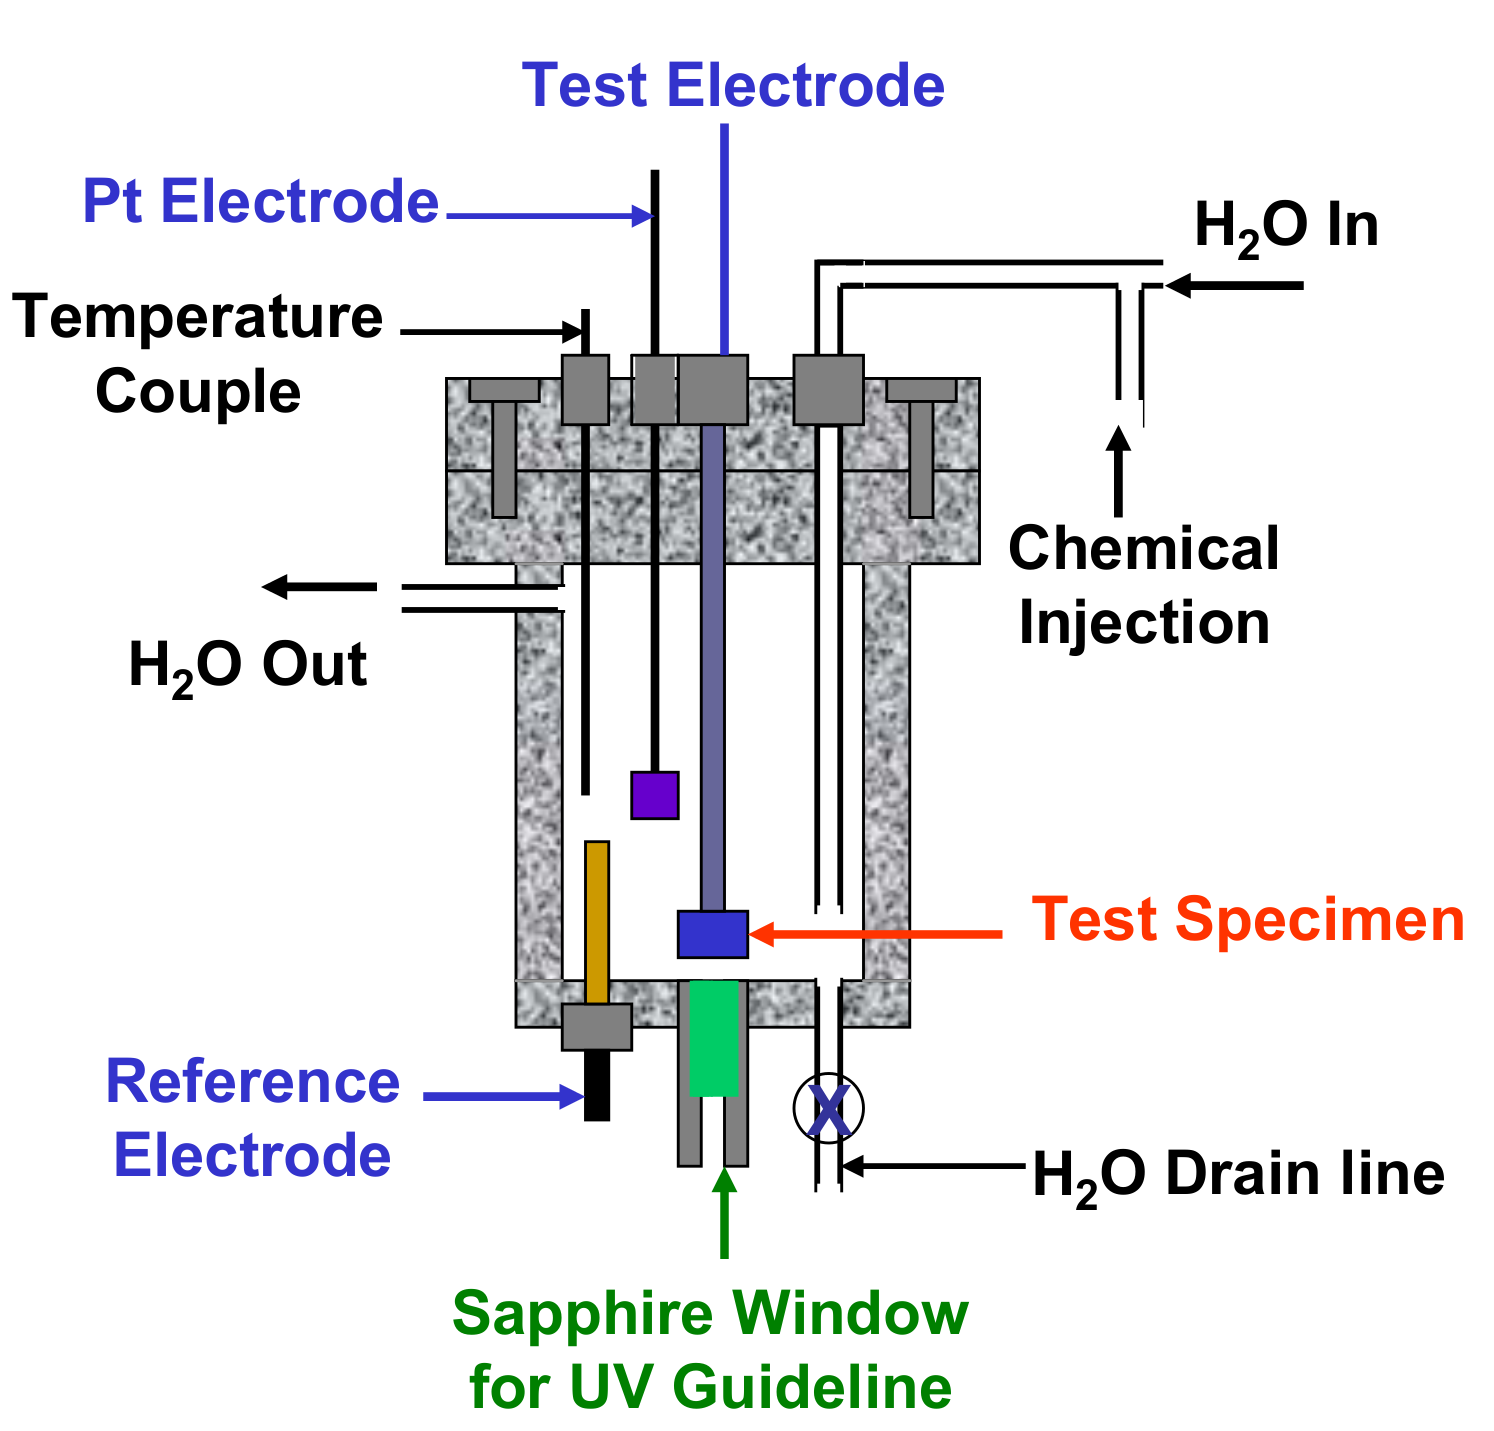
\includegraphics[width=0.5\textwidth]{Kim_2010_Fig2.png} 
            \caption[Représentation schématique de l'autoclave équipé d'un hublot.]
            {Représentation schématique de l'autoclave équipé d'un hublot \citep{Kim2010}.} 
            \label{fig:kim_autoclave} 
        \end{figure}

    \subsection{Résultats}

    La figure~\ref{fig:kim_ecp_vs_time_H2_O2} montre l’évolution des potentiels électrochimiques des différents
    matériaux selon que l’électrolyte contient \SI{0.15}{\ppm} de $\rm H_2$ ou \SI{1.1}{\ppm} d’$\rm O_2$. Dans un
    environnement peu oxydant, soit \SI{0.15}{\ppm} de $\rm H_2$, tous les matériaux présentent des potentiels
    électrochimiques similaires. Lorsque l’environnement est plus oxydant, soit \SI{1.1}{\ppm} d’$\rm O_2$, des
    différences notables apparaissent en termes de valeurs de potentiel électrochimique : le potentiel du Zircaloy-2 est
    plus cathodique que celui des autres matériaux. Ce premier résultat suggère que le phénomène de Shadow Corrosion
    peut être potentiellement une conséquence de la séparation des potentiels en milieu oxygéné caractéristique des REB.
    \citet{Cox2005} suggère que l’ajout de $\rm H_2$ à hauteur de 10~$\rm cc \, kg^{-1}$ pourrait éliminer l’apparition de la Shadow
    Corrosion en fixant le potentiel électrochimique des matériaux au potentiel de l’hydrogène.

    \begin{figure}[H] 
            \centering 
            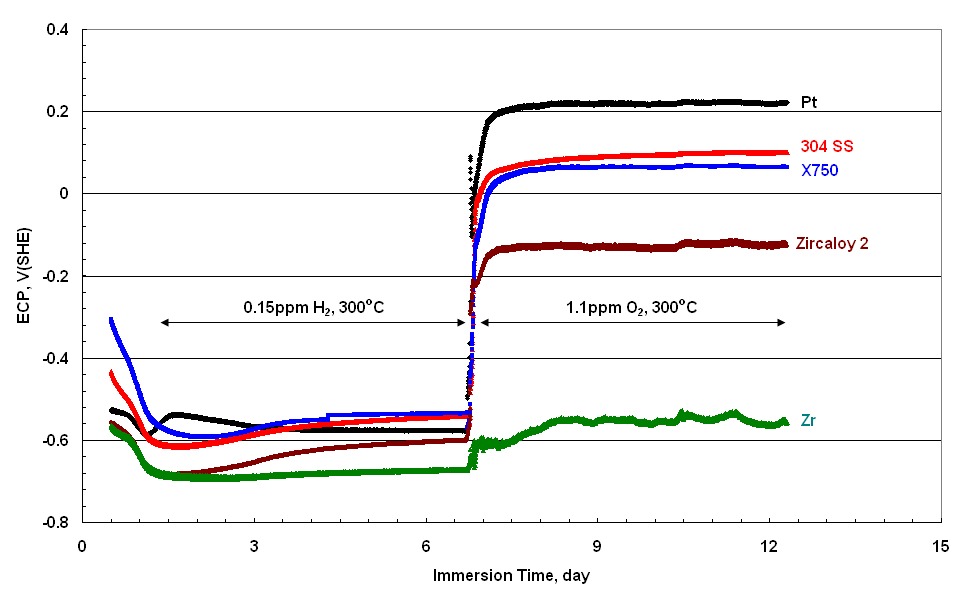
\includegraphics[width=0.85\textwidth]{Kim_2010_Fig3.png} 
            \caption[Evolution des potentiels électrochimiques de l’alliage Zircaloy-2, de l’acier inoxydable 304,
            de l’alliage de nickel X750 et du Pt dans l'eau à \Tkim\ contenant \SI{0.15}{\ppm} de \Hyd\ ou \SI{1.1}{ppm}
        d’\Oxy.]
            {Evolution des potentiels électrochimiques de l’alliage Zircaloy-2, de l’acier inoxydable 304,
            de l’alliage de nickel X750 et du Pt dans l'eau à \Tkim\ contenant \SI{0.15}{\ppm} de \Hyd\ ou \SI{1.1}{ppm}
        d’\Oxy \citep{Kim2010}.} 
            \label{fig:kim_ecp_vs_time_H2_O2} 
        \end{figure}


    La figure~\ref{fig:kim_ecp_vs_time_O2_UV} présente l’évolution des potentiels électrochimiques de l’alliage 
    Zircaloy-2 et de l’alliage de nickel X750 sous illumination UV--Visible intermittente. Le potentiel du Zircaloy-2 diminue vers
    des valeurs plus cathodiques alors que le potentiel de l’alliage X750 augmente vers des valeurs plus anodiques.
    Cette
    variation des potentiels électrochimiques augmente ainsi la différence de potentiel entre les matériaux et par
    conséquent l'intensité d'un éventuel couplage galvanique comme
    illustré en figure~\ref{fig:kim_current_vs_time_O2_UV}. Le sens de variation des potentiels électrochimiques
    sous illumination UV--Visible indique que la couche zircone présente une semiconduction de type \emph{n} alors que l’oxyde 
    formé sur l’alliage X750 présente une semiconduction de type \emph{p} \citep{Memming2008}.
    Cependant, la normalisation
    par rapport à la surface de l'échantillon de Zircaloy-2 (\SI{\sim 1.6}{\square\centi\meter}) des courants de couplage
    mesurés sur la figure \ref{fig:kim_current_vs_time_O2_UV}, fait apparaître des densités de courants ne dépassant
    pas la barre des \SI{1}{\micro\ampere\per\square\centi\meter} dans le cas du couple Zircaloy-2/X750 et donc la
    densité de courant de couplage sous illumination UV--Visible 
    n'est pas supérieure aux valeurs typiques qui sont mesurables en autoclave (\S\ref{subsubsec:oxidation_kinetics}, figure
    \ref{fig:Zy2_Kinetics_vs_T_J}).

    
    \begin{figure}[H] 
        \centering 
        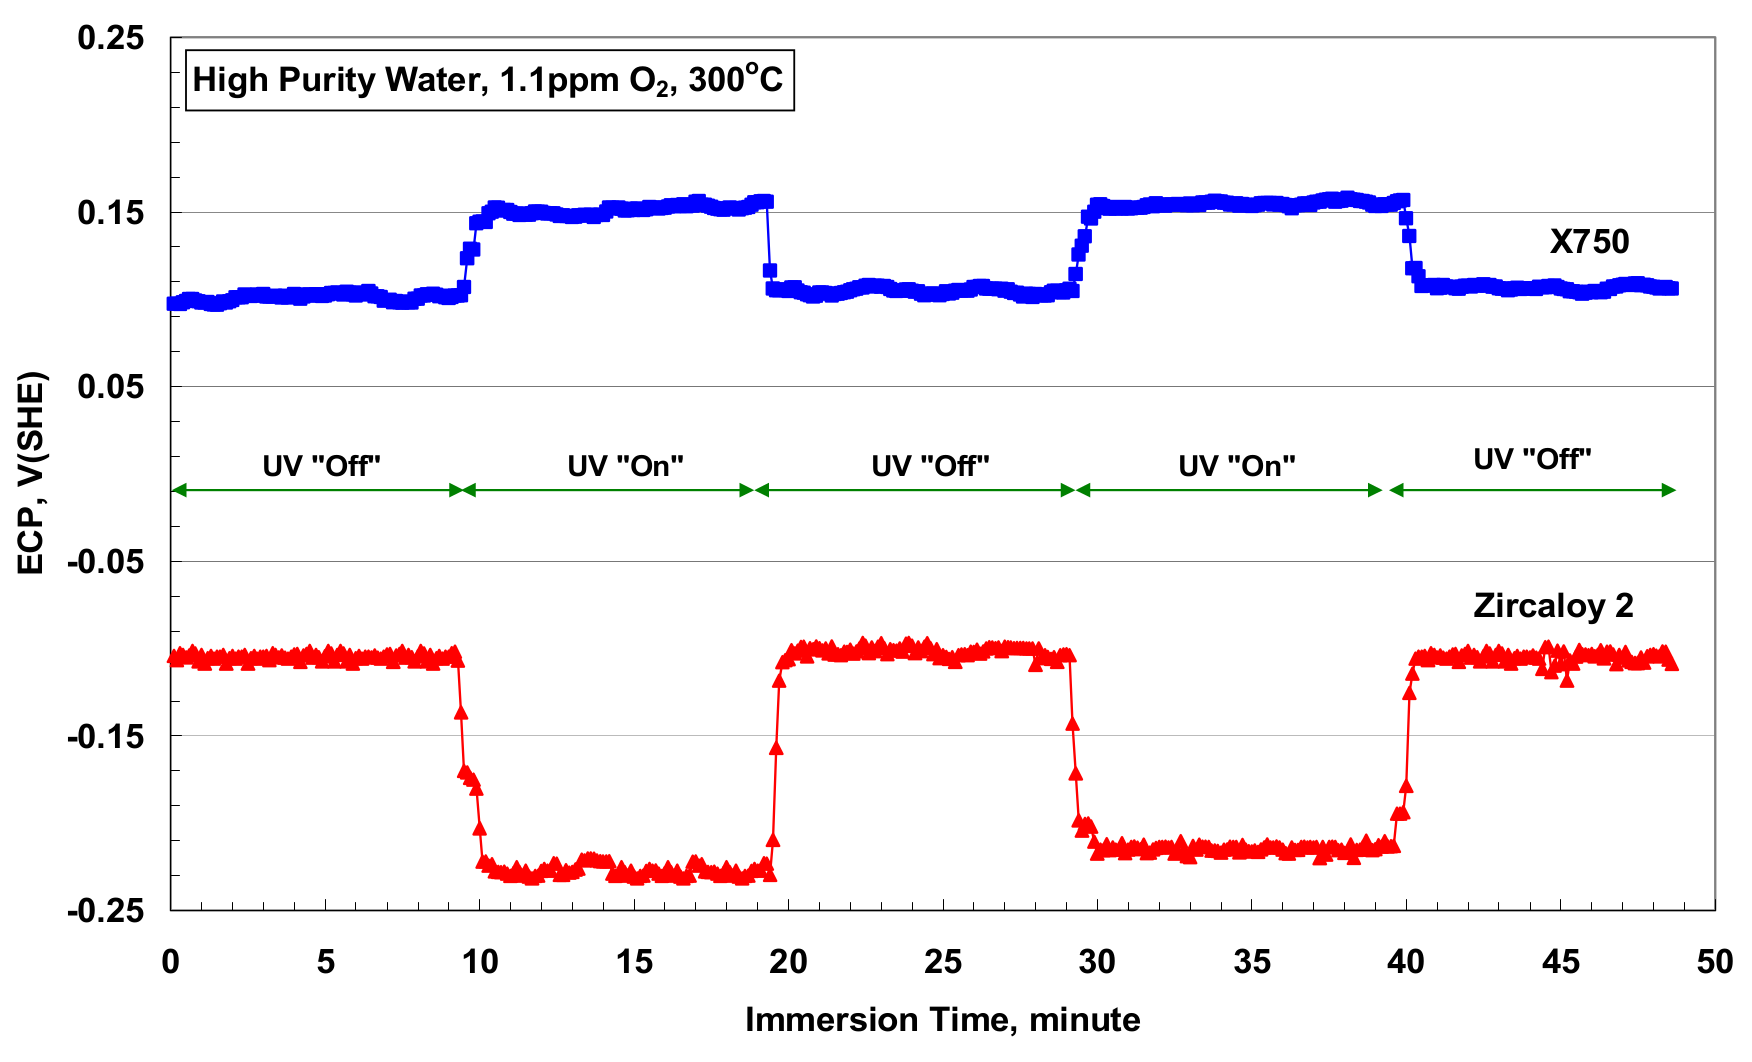
\includegraphics[width=0.85\textwidth]{Kim_2010_Fig6.png} 
        \caption[Potentiels électrochimiques mesurés sur les alliages Zircaloy-2 et X750 dans l'eau à
        \SI{300}{\degreeCelsius} contenant \SI{1.1}{ppm} d'oxygène avec ou sans illumination UV--Visible.]
        {Potentiels électrochimiques mesurés sur les alliages Zircaloy-2 et X750 dans l'eau à
        \SI{300}{\degreeCelsius} contenant \SI{1.1}{ppm} d'oxygène avec ou sans illumination UV--Visible \citep{Kim2010}.} 
        \label{fig:kim_ecp_vs_time_O2_UV} 
    \end{figure}

    \begin{figure}[H]
        \centering
        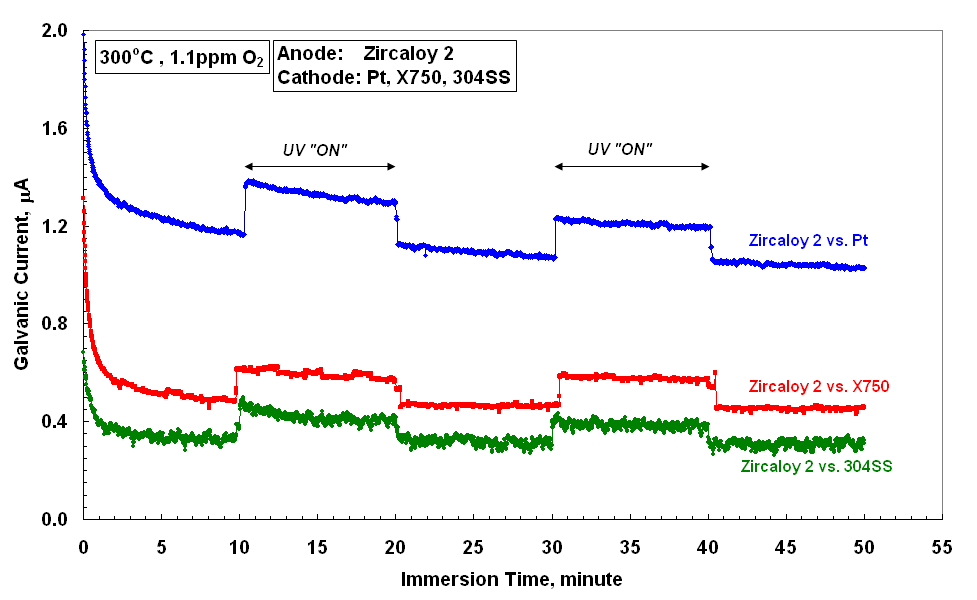
\includegraphics[width=0.85\textwidth]{Kim_2010_Fig13.png} 
        \caption[Courants de couplage mesurés pour les couples Zircaloy-2/X750, Zircaloy-2/Pt et Zircaloy-2/304SS dans l'eau à
        \SI{300}{\degreeCelsius} contenant \SI{1.1}{ppm} d'oxygène avec ou sans illumination UV--Visible.]
        {Courants de couplage mesurés pour les couples Zircaloy-2/X750, Zircaloy-2/Pt et Zircaloy-2/304SS dans l'eau à
        \SI{300}{\degreeCelsius} contenant \SI{1.1}{ppm} d'oxygène avec ou sans illumination UV--Visible \citep{Kim2010}.} 
        \label{fig:kim_current_vs_time_O2_UV} 
    \end{figure}

    L’auteur n’étudie pas l’influence de la longueur d'onde (l’énergie) de la lumière incidente sur la réponse
    en termes de potentiel et de courant. 
    La zircone est l'oxyde majoritaire qui se forme sur la surface de l'alliage Zircaloy-2. 
    Néanmoins, des oxydes minoritaires y sont
    également présents tels que des oxydes de fer, de chrome et/ou spinelles dont les largeurs de bande interdite sont
    inférieures à celle de la zircone \citep{Atmani2008,Loucif2013}. Dans le cas des alliages de nickel, la couche
    d'oxyde est duplex avec une couche interne riche en chrome et une couche externe formée de spinelle de
    nickel, fer et chrome \citep{Marchetti2006}.
    Par conséquent, l’illumination UV--Visible modifie également
    le comportement électrochimique de ces oxydes "mineurs". En d’autres termes, la modification de comportement
    électrochimique, sous illumination UV--Visible, observée dans cette étude est la résultante de la contribution de l’oxyde
    majoritaire mais également de la contribution de tous les oxydes minoritaires.
    Une manière de séparer ces différentes contributions est de réaliser des caractérisations par photoélectrochimie
    (communément désignée par PEC) au photopotentiel ou au photocourant.


    Le paragraphe \ref{sec:state_of_art_PEC} qui suit donne les bases théoriques nécessaires à la compréhension de ce
    type de caractérisations, ainsi que quelques exemples d'applications à la caractérisation de couches d'oxydation
    thermiques. Nous y reviendrons plus en détail au chapitre \ref{chap:design}.

    
    

%%%%%%%%%%%%%%%%%%%%%%%%%%%%%%%%%%%%%%%%%%%%%%%%%%%%%%%%%%%%%%%%%%%%%%%%%%%%%%%%%%%%%
%%%%%%%%%%%%%%%%%%%%%%%%%%%%%%%%%%%%%%%%%%%%%%%%%%%%%%%%%%%%%%%%%%%%%%%%%%%%%%%%%%%%%
\section{Caractérisations photoélectrochimiques}\label{sec:state_of_art_PEC}
    
    La photoélectrochimie utilise l'effet photovoltaïque à l'interface entre un semiconducteur et un électrolyte découvert par
    \citet{Becquerel1839} en 1839. La première expérience a été réalisée avec une électrode d'argent sur laquelle une
    couche d'oxyde s'était développée. Cette dernière a été mise dans une solution acide et connectée à une électrode de
    platine. Lors de l'illumination, un photopotentiel et un photocourant ont été observés. Les premières études de
    compréhension des processus physico-chimiques se produisant à l'interface semiconducteur/électrolyte et à l'origine
    de photopotentiel ou de ce photocourant ont été réalisées bien plus tardivement 
    \citep{Gerischer1966, Copeland1942, Stimming1986}. 

    La photoélectrochimie est, aujourd'hui entre autres, un outil de caractérisations \emph{in-situ} \citep{Fujishima1972, Gratzel2001}, 
    ou \emph{ex-situ} \citep{Carpenter1989, Sunseri1995, Boschloo2001} de matériaux semiconducteurs tels que les oxydes
    formés sur les alliages métalliques, les sulfures et les carbures. Cette technique permet de déterminer des
    propriétés optiques et électroniques des semiconducteurs tels que leur largeur de bande interdite ainsi que leur
    type de semiconduction.
    Elle permet également de déterminer des paramètres de l'interface semiconducteur/électrolyte tels que les positions
    des bords de bande au contact de l'électrolyte. 
    
    Les notions de base de la photoélectrochimie sont présentées dans la suite avec des exemples d'application de la photoélectrochimie
    sur des alliages de zirconium et de nickel. Le détail du développement théorique est très largement décrit dans la
    littérature \citep{Marcus2006, Memming2008, Gerischer1985, Morrison1980, Bard2002, Sato1998}.
    On notera que, l'ensemble des notions qui vont être introduites dans la suite 
    font les hypothèses suivantes:
    \begin{itemize}
        \item le semiconducteur est considéré comme idéal c'est-à-dire cristallin, homogène, semi-infini
        \item la constante diélectrique du semi-conducteur ($\epsilon$) est indépendante de la fréquence
        \item l'interface du semiconducteur est plane
        \item la capacité de la couche de Helmholtz ($C_\Hm$) est très grande devant celle de la région de la charge
        d'espace du semiconducteur
        \item la variation de la chute de potentiel dans la couche de Helmholtz en fonction du
        potentiel imposé ou du dopage du semi-conducteur est négligeable.
    \end{itemize}

    Les oxydes ou les films passifs formés sur les alliages, lors du vieillissement de ces derniers, respectent très
    rarement l'ensemble des conditions énoncées ci-dessus, mais la littérature montre que les modèles développés ci-après
    restent souvent applicables approximativement, mais avec profit.


    \subsection{Notions de base sur les semiconducteurs}\label{subsec:basics_semiconductors}
    
    \subsubsection{Structure de bandes électroniques}\label{subsubsec:band_model}

    Les solides sont généralement classés en trois catégories: \emph{conducteurs}, \emph{semiconducteurs} et
    \emph{isolants}.
    Chacune de ces catégories peut être représentée par une structure de bande d'énergie électronique illustrée en figure
    \ref{fig:band_model}. Les bandes de \emph{valence} et de \emph{conduction} sont des bandes d'énergie permises pour les
    électrons. Elles sont séparées par une bande d'énergie nommée \emph{gap} ou \emph{bande interdite} qui ne
    comprend aucun état d'énergie électronique permise: sa largeur est notée $\E_g$. La répartition des électrons dans
    ces
    bandes est décrite par la position du niveau de Fermi noté $\E_F$. Ce dernier représente l'énergie la plus haute que peut occuper
    un électron à \SI{0}{\kelvin}, il est l'équivalent du potentiel électrochimique des électrons dans la phase solide. 
    La plus basse énergie de la bande de conduction est notée $\E_c$ alors que l'énergie
    la plus élevée de la bande de valence est notée $\E_v$.

     \begin{figure}[H]
        \centering
        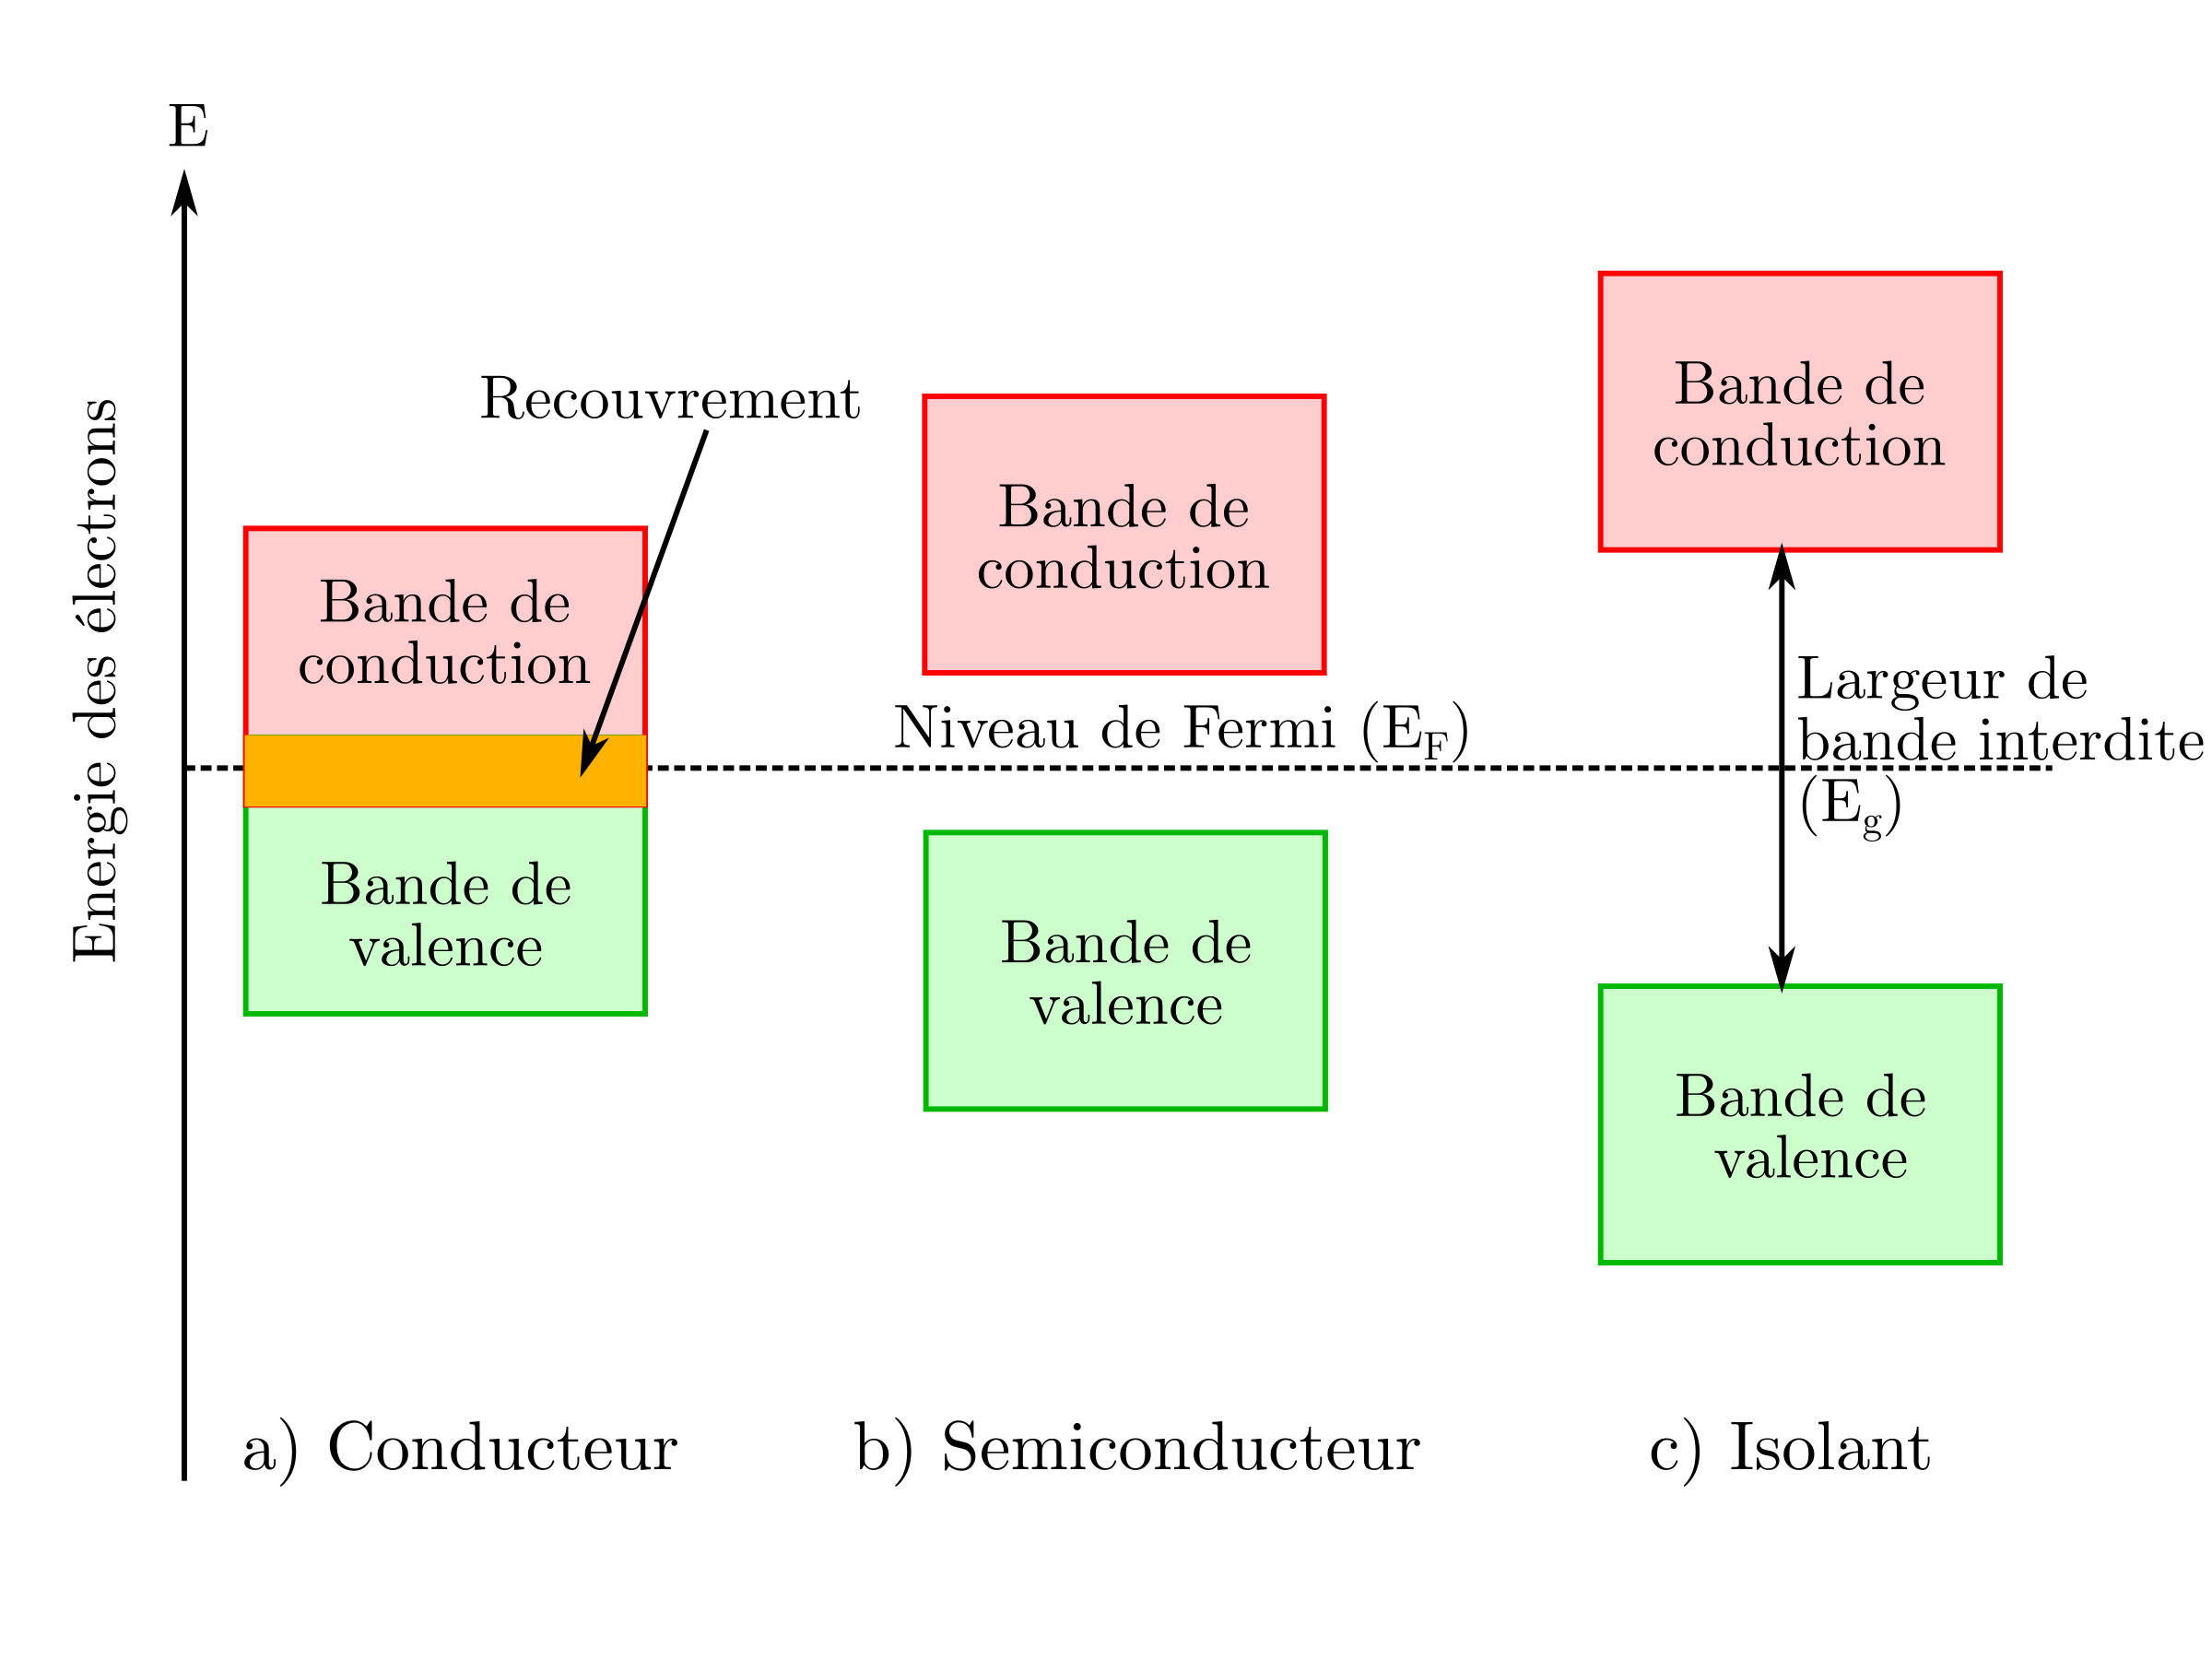
\includegraphics[width=0.65\textwidth]{Band_Model.png}
        \caption[Représentation schématique des structures de bandes électroniques:
        a) conducteur, 
        b) semiconducteur,
        c) isolant.]
        {Représentation schématique des structures de bandes électroniques (d'après \citet{Marucco2006}):
        a) conducteur, 
        b) semiconducteur,
        c) isolant.}
        \label{fig:band_model}
    \end{figure}

    La conduction électronique est due soit aux mouvements, dans la bande de
    conduction, des électrons chargés négativement soit aux mouvements, dans la bande de valence, des trous chargés
    positivement ou bien aux deux simultanément. La conduction électronique dépend donc du nombre de porteurs de charge
    disponibles dans la bande de conduction et dans la bande de valence. 
    Dans le cas d'un conducteur, la bande permise occupée d'énergie la plus élevée est partiellement remplie, on dit
    quelquefois que les bandes de valence et de conduction se trouvent en position de recouvrement.
    La distinction, en termes de conduction électronique, entre un semiconducteur et un isolant est plus floue puisqu'elle 
    dépend de la largeur du gap et de l'énergie apportée par l'environnement aux électrons de la bande de valence pour
    passer dans la bande de conduction. 
    
    Dans les semiconducteurs, les porteurs de charge peuvent être générés de trois manières différentes:
    \emph{excitation thermique}, \emph{photoexcitation} et \emph{dopage}. La figure \ref{fig:excitation_carrier} illustre
    de manière schématique les trois mécanismes de générations des porteurs de charge dans les bandes de valence ou de
    conduction. Pour des gaps faibles,
    l'excitation thermique peut expulser un électron de la bande de valence vers la bande de conduction. Dans le cas de la
    photoexcitation, un électron peut être expulsé de la bande de valence vers la bande de conduction lorsqu'un photon
    incident absorbé possède une énergie supérieure au gap. Le dopage, quant à lui, consiste à introduire des niveaux d'énergie
    supplémentaires situés entre la bande de valence et la bande de conduction.

    \begin{figure}[H]
        \centering
        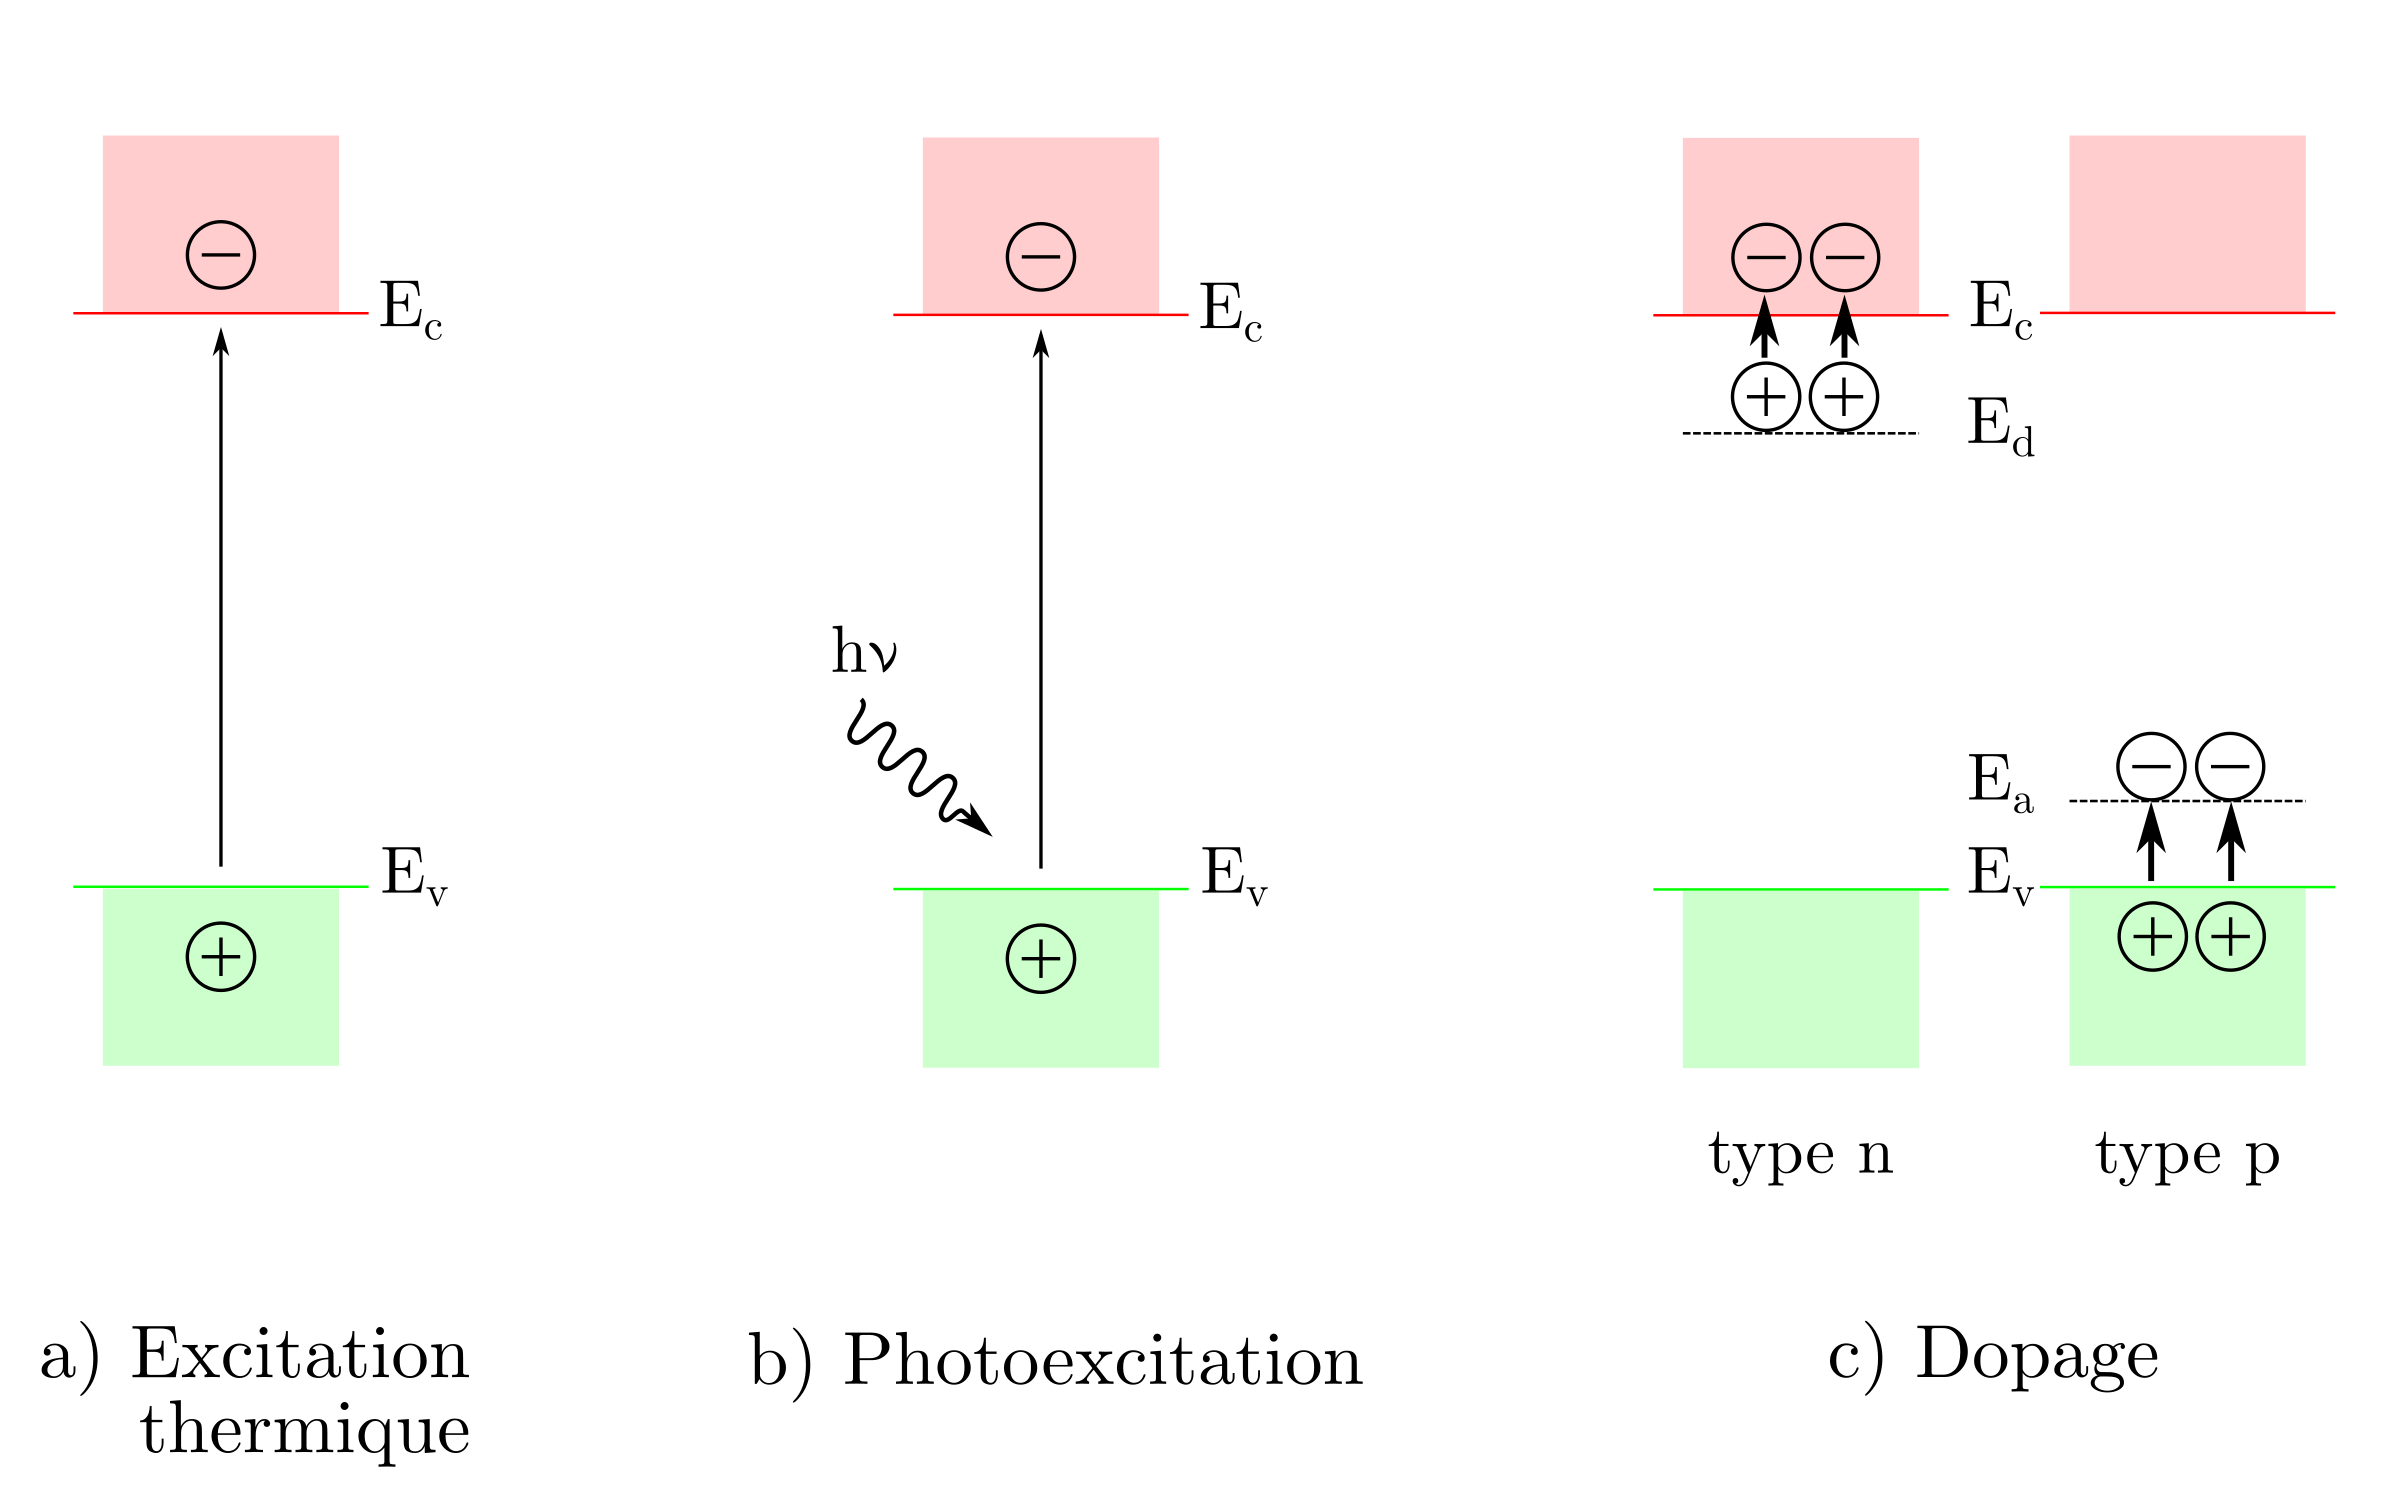
\includegraphics[width=0.85\textwidth]{Excitation_Carrier.png}
        \caption[Représentation schématique des mécanismes de génération des porteurs de charge dans des
        semiconducteurs ou des isolants:
        a) excitation thermique,
        b) photoexcitation,
        c) dopage.]
        {Représentation schématique des mécanismes de génération des porteurs de charge dans des
            semiconducteurs ou des isolants (d'après \citet{Finklea1983}):
        a) excitation thermique,
        b) photoexcitation,
        c) dopage.}
        \label{fig:excitation_carrier}
    \end{figure}

    Le dopage peut être dû à une modification de la stoechiométrie du semiconducteur, ou l'introduction d'impuretés
    dans le réseau du
    semiconducteur. Dans le cas des semiconducteurs de type \emph{n}, les niveaux d'énergie donneurs d'électrons
    $\E_d$ se situent près
    de la bande de conduction. Les électrons des niveaux d'énergie donneurs rejoignent la bande de conduction par
    excitation thermique. Par conséquent, les porteurs de charge majoritaires sont des électrons chargés négativement
    mobiles dans la bande de conduction.
    De manière similaire, les niveaux d'énergie accepteur d'électrons $\E_a$ des semiconducteurs de type \emph{p} se
    situent près de la
    bande de valence. Ces derniers capturent les électrons de la bande de valence créant ainsi des trous. Dans ce cas de
    figure, les porteurs de charge majoritaires sont des trous chargés positivement mobiles dans la bande de valence.
    La classification des semiconducteurs, type \emph{p} ou type \emph{n}, indique donc le signe des porteurs de
    charges mobiles
    majoritaires. Les semiconducteurs non dopés sont appelés semiconducteurs intrinsèques.

    Le niveau de Fermi ($\E_F$) dans les semiconducteurs intrinsèques est situé au milieu du gap. Le dopage de
    type \emph{n} et \emph{p} déplace le niveau de Fermi vers les bords des bandes de conduction $\E_c$ et de valence
    $\E_v$, respectivement.
    La figure \ref{fig:fermi_position} illustre la position du niveau de Fermi en fonction du type de semiconducteur.


     \begin{figure}[H]
        \centering
        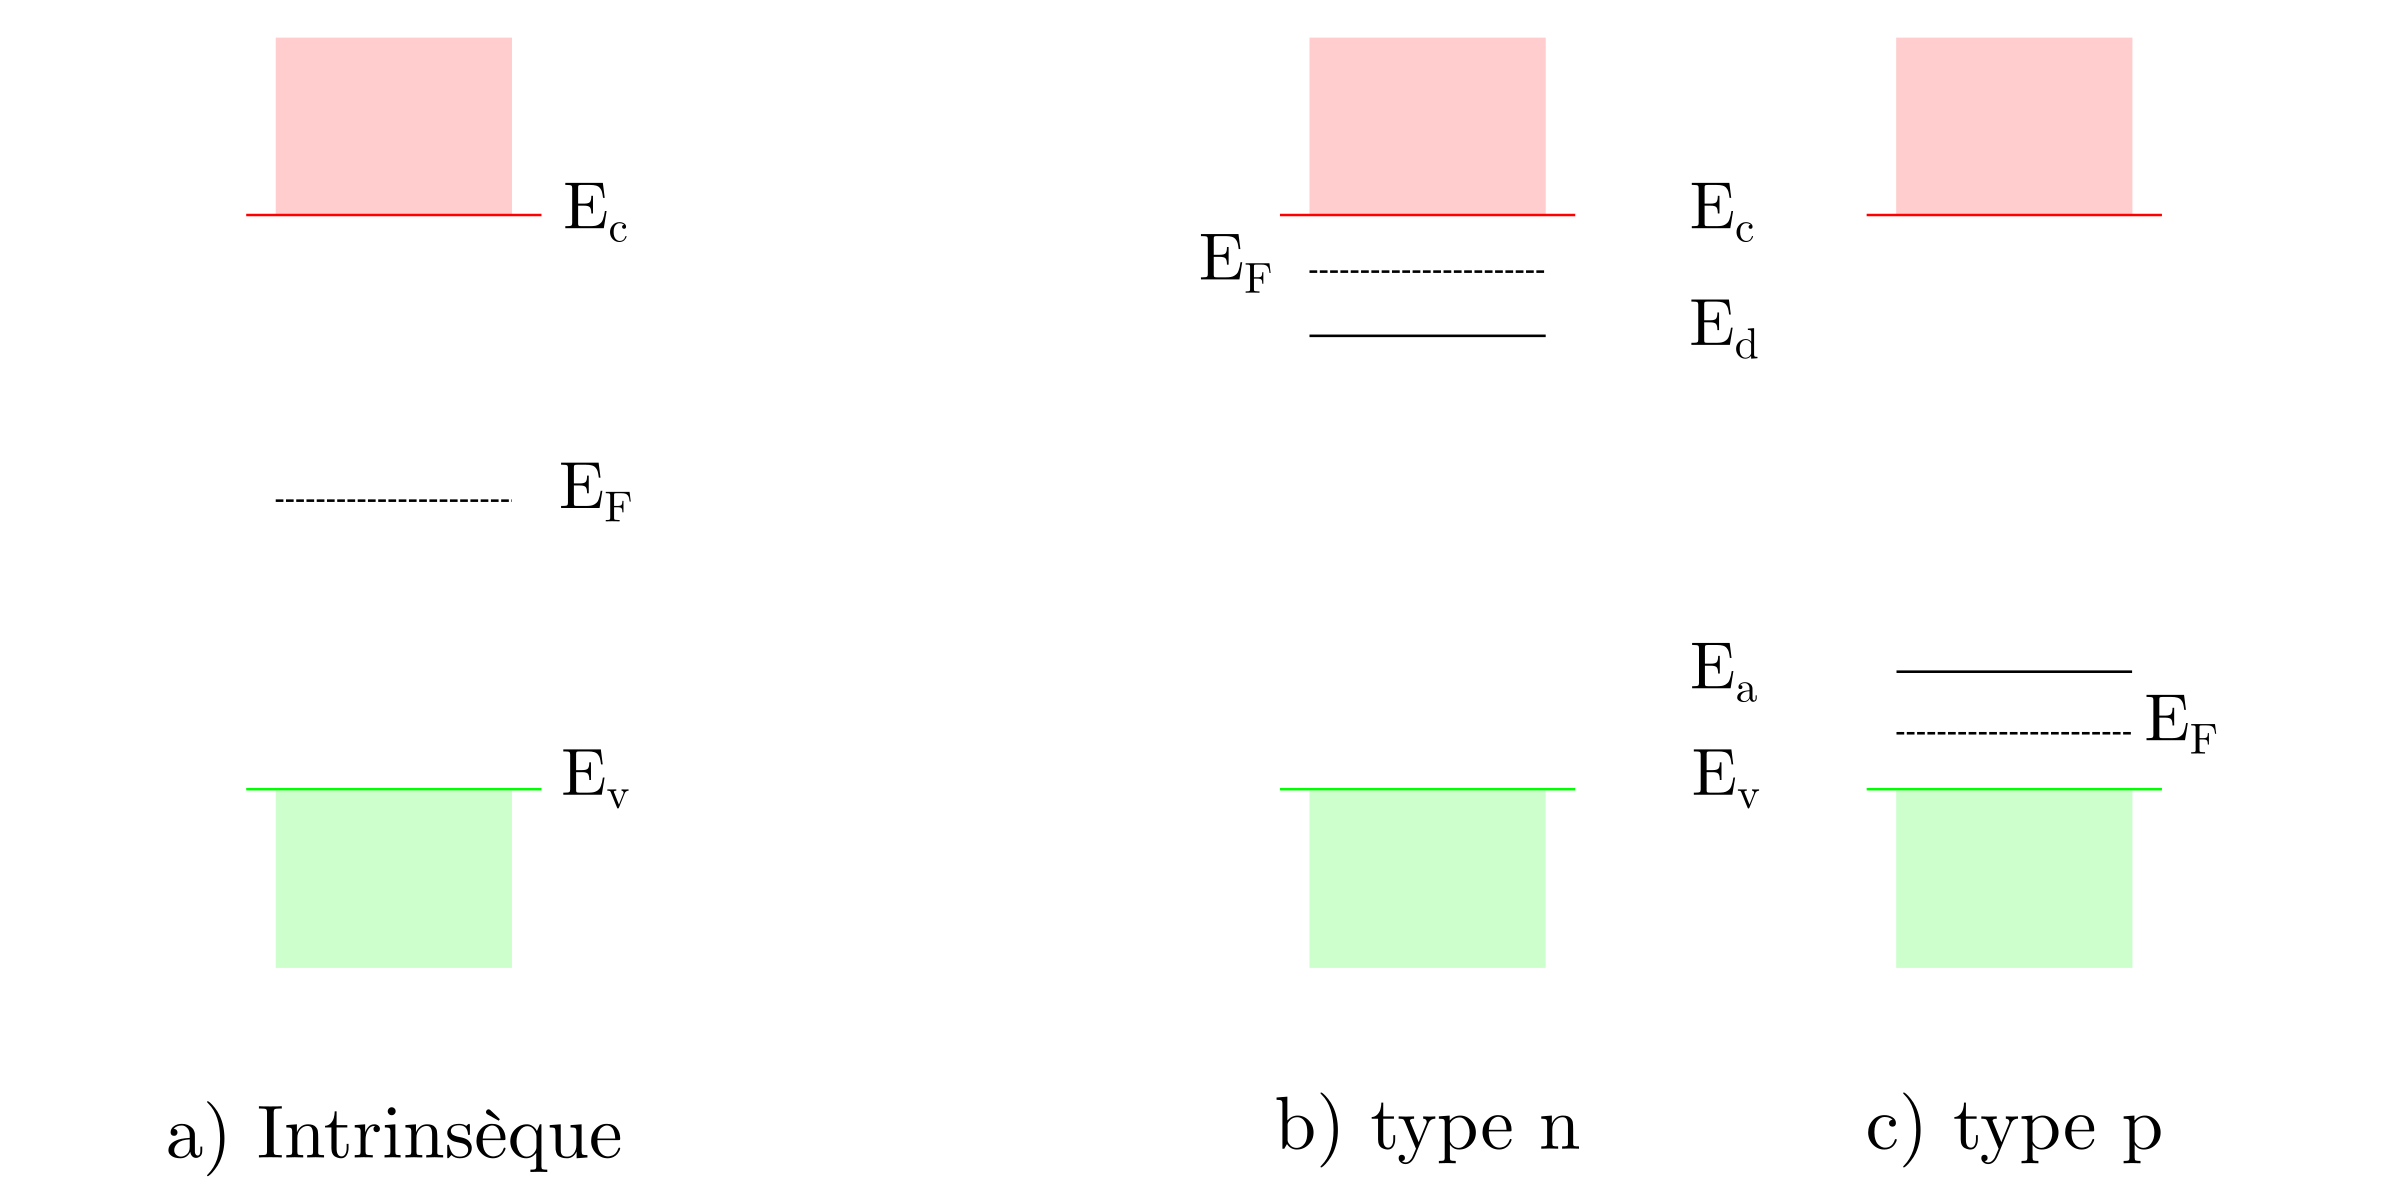
\includegraphics[width=0.85\textwidth]{Fermi_Position.png}
        \caption[Représentation schématique de la position du niveau de Fermi en fonction du type de semiconducteur:
        a) intrinsèque,
        b) type \emph{n},
        c) type \emph{p}.]
        {Représentation schématique de la position du niveau de Fermi en fonction du type de semiconducteur
            (d'après \citet{Finklea1983}):
        a) intrinsèque,
        b) type \emph{n},
        c) type \emph{p}.}
        \label{fig:fermi_position}
    \end{figure}


    
    \subsubsection{Interface semiconducteur/électrolyte à l'obscurité}
    \label{subsec:semiconductor_electrolyte_contact_dark}
     
    Lorsqu'un semiconducteur est mis en contact avec un électrolyte, un gradient de potentiel s'établit à l'interface. Le
    profil du potentiel à l'interface est illustré par la figure \ref{fig:interfacial_potential_gradient}. 
    
    \begin{figure}[H]
        \centering
        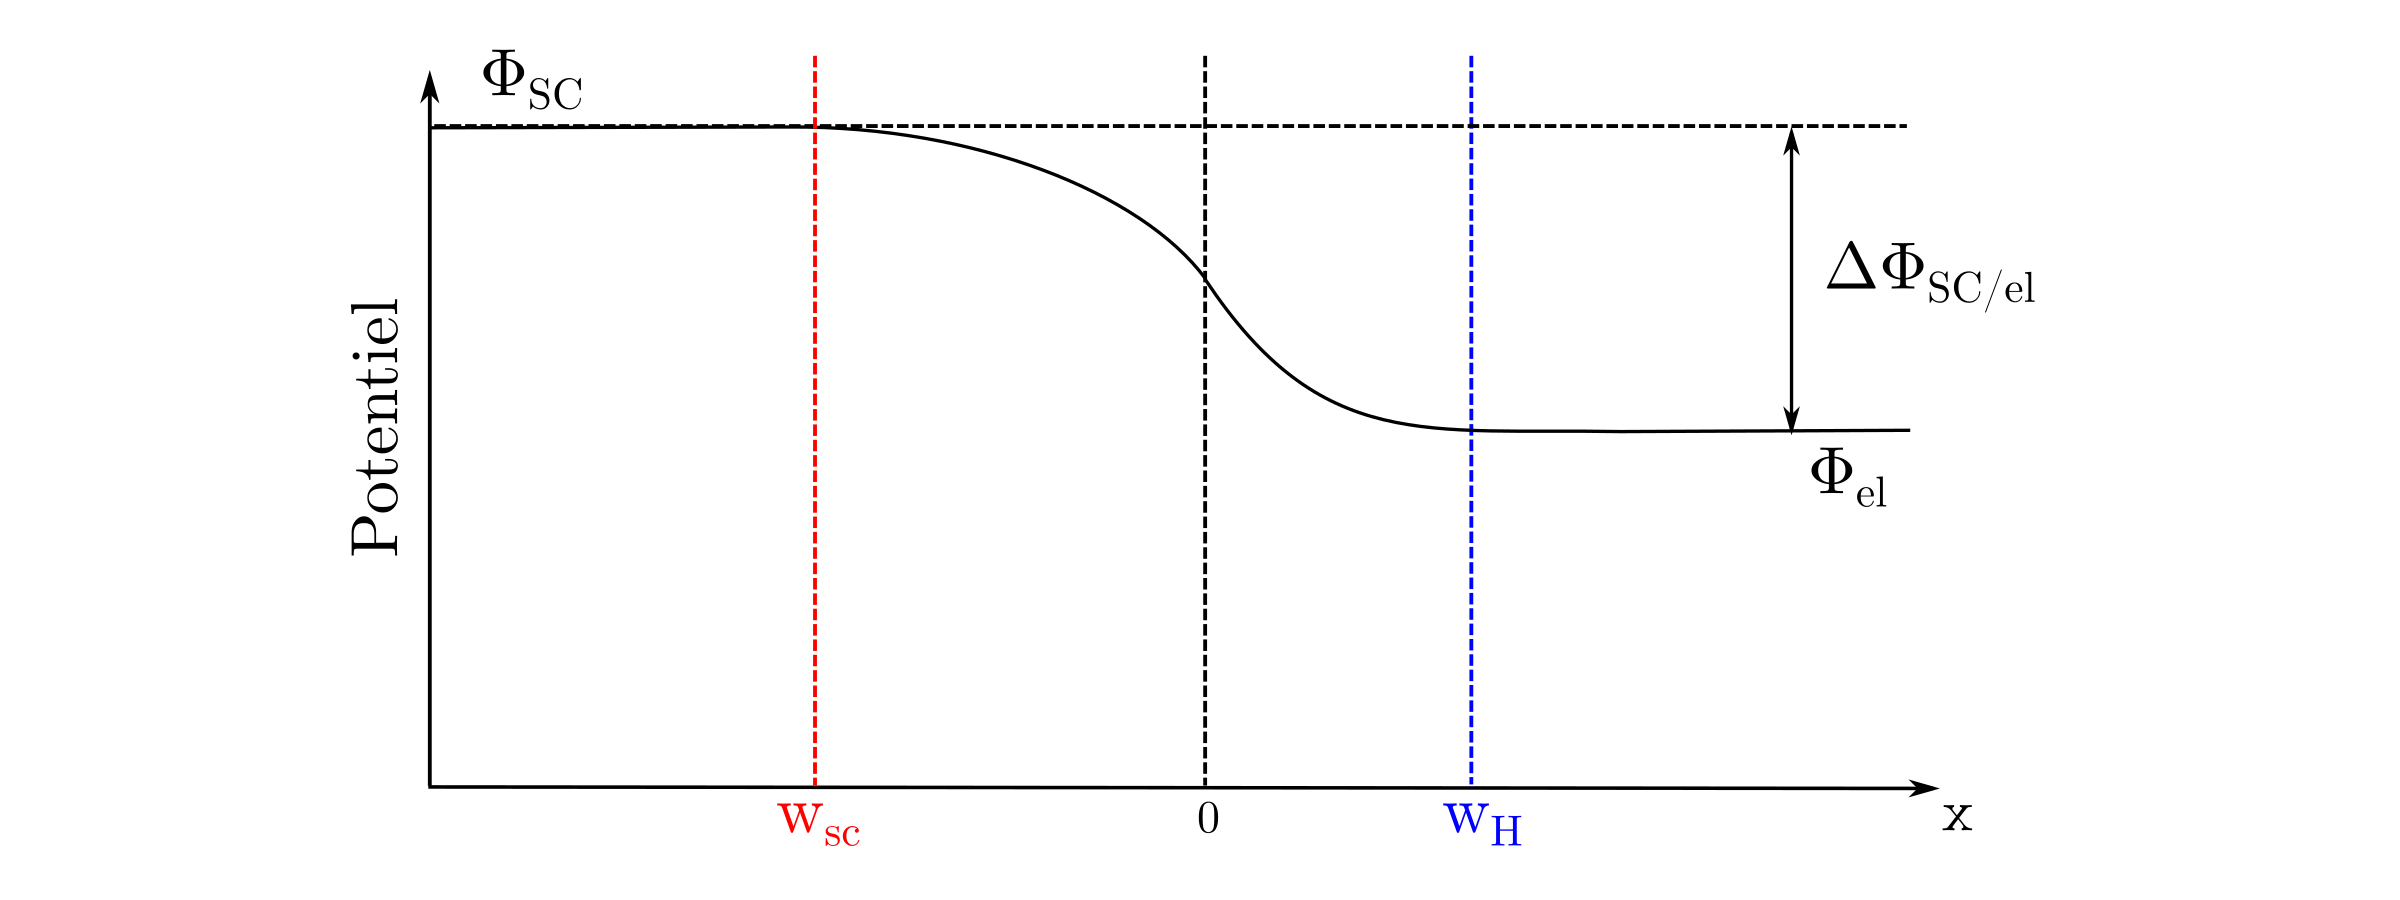
\includegraphics[width=0.85\textwidth]{Interfacial_Potential_Gradient.png}
        \caption[Gradient de potentiel à l'interface semiconducteur/électrolyte.]
        {Gradient de potentiel à l'interface semiconducteur/électrolyte (d'après \citet{Marcus2006}). $\Phi _{\SC}$ et
        $\Phi _{\el}$
        correspondent aux potentiels dans le semiconducteur et l'électrolyte, respectivement. $\Delta \Phi _{\SC/\el}$ correspond à la
        différence de potentiel entre le semiconducteur et l'électrolyte. $w_{\SC}$ et $w_{\Hm}$ correspondent aux
        épaisseurs de la charge d'espace et de la double couche électrochimique, respectivement.}
        \label{fig:interfacial_potential_gradient}
    \end{figure}
    
    En fonction du niveau de Fermi de
    l'électrolyte par rapport aux bords des bandes de valence et de conduction du semiconducteur, le transfert de charge
    transitoire peut mener à trois situations principales. La situation de bande plate est obtenue lorsque le niveau de Fermi
    dans l'électrolyte correspond à celui du semiconducteur. Dans cette situation, il n'y pas de
    gradient de potentiel dans le semiconducteur, on parle de situation de bandes plates. Si les deux niveaux de Fermi
    ne sont pas alignés, une courbure des bandes
    dans le semiconducteur apparaît au voisinage de l'interface semiconducteur/électrolyte. 
    Cette courbure des bandes entraîne soit un appauvrissement soit
    une accumulation des porteurs de charge majoritaires au voisinage de l'interface.
    L'extension spatiale de la zone d'appauvrissement
    ou d'accumulation est appelée région de charge d'espace (figure \ref{fig:bending_example}).

     \begin{figure}[H]
        \centering
        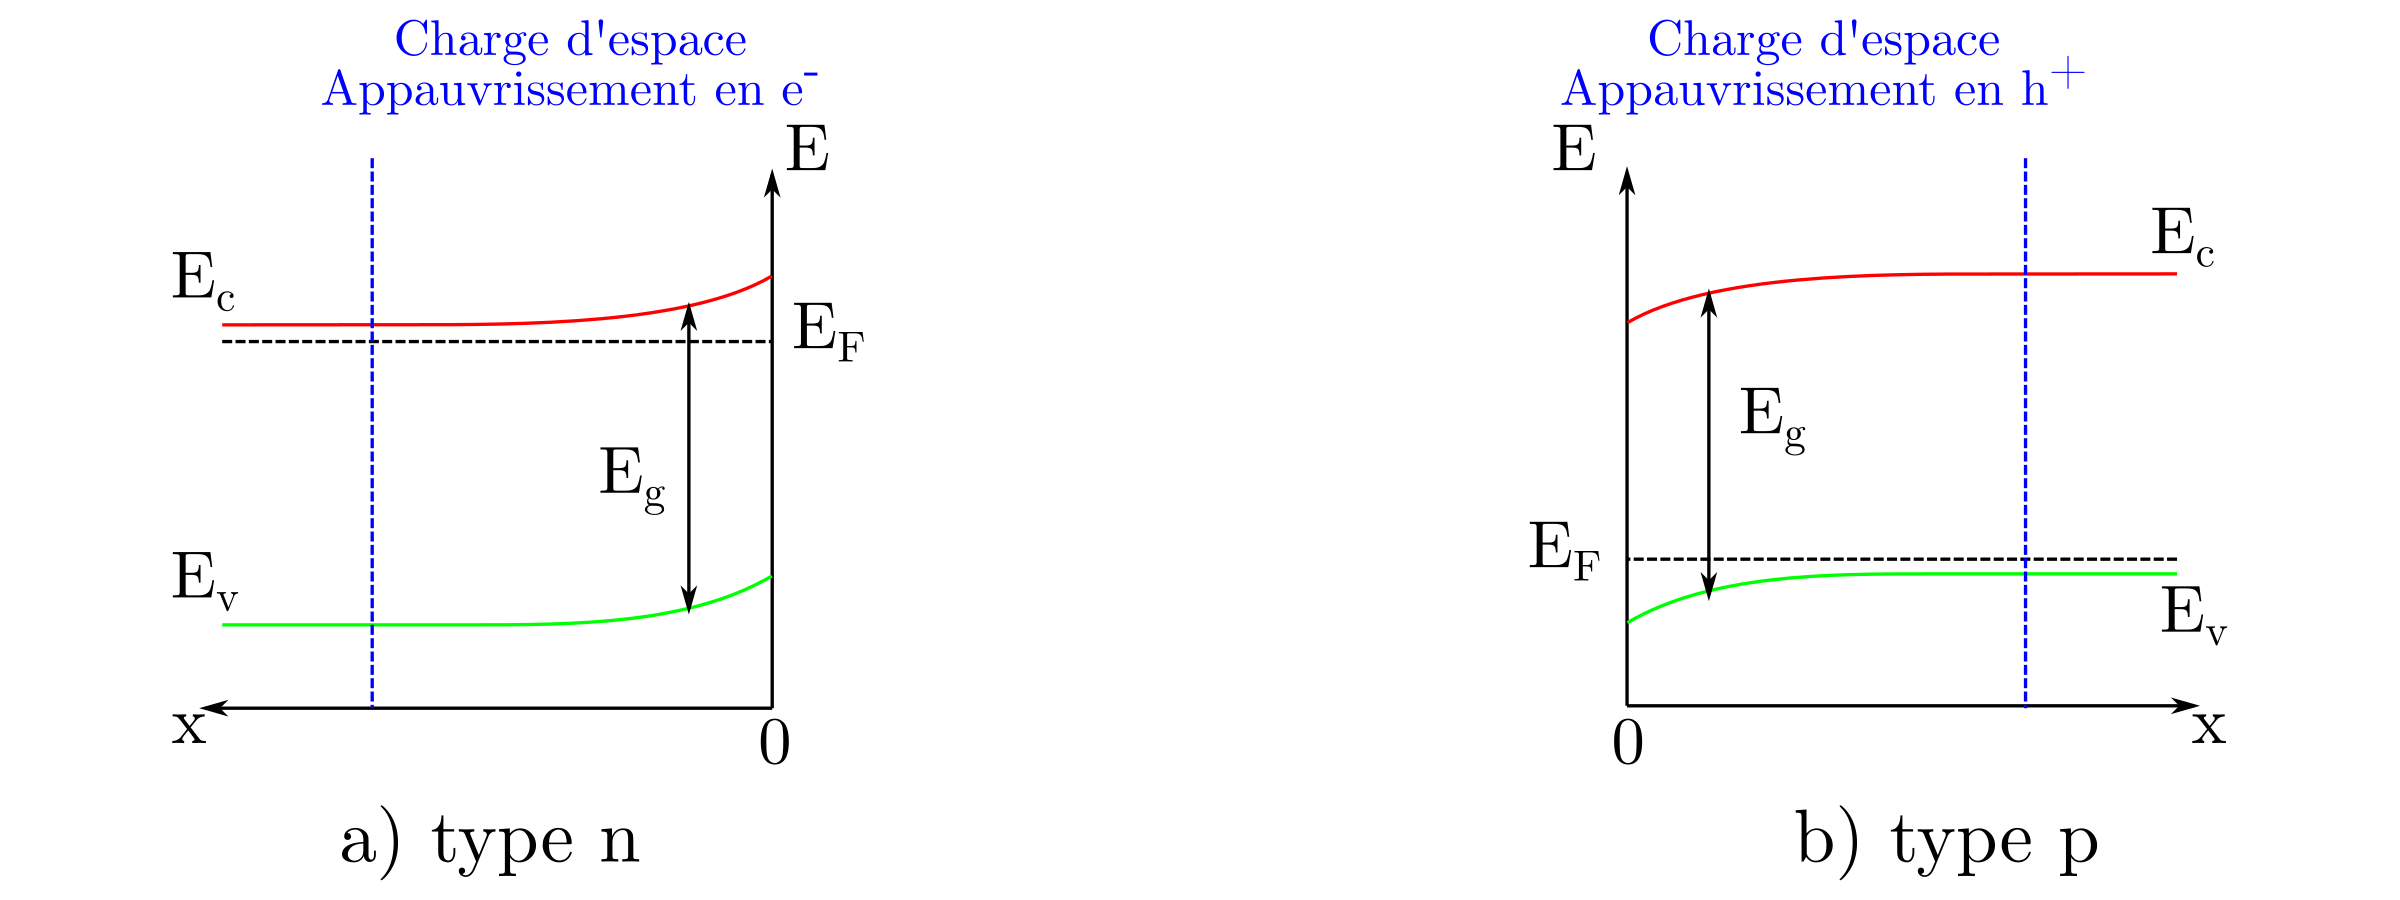
\includegraphics[width=0.85\textwidth]{Bending_Example.png}
        \caption[Représentation schématique d'une région de charge d'espace en situation d'appauvrissement en porteurs 
        de charge majoritaires pour un semiconducteur en contact avec un électrolyte: a)
        type \emph{n}, b) type \emph{p}.]
        {Représentation schématique d'une région de charge d'espace en situation d'appauvrissement en porteurs 
            de charge majoritaires pour un semiconducteur en contact avec un électrolyte (d'après \citet{Bard2002, Memming2008}): a)
        type \emph{n}, b) type \emph{p}.}
        \label{fig:bending_example}
    \end{figure}

    Les situations d'accumulation et d'appauvrissement et de bandes plates dans la région de charge d'espace
    peuvent être obtenues par polarisation du semiconducteur par rapport à une référence dans l'électrolyte. Si les
    hypothèses listées au début de ce paragraphe sont respectées, la polarisation ne modifie
    pas la position en énergie des bords de bande en surface, $\E_{cs}$ et $\E_{vs}$.
    La polarisation appliquée ne modifiera donc que les courbures de bande dans la région de charge d'espace.
    En fonction du potentiel appliqué (U) par rapport au potentiel correspondant à la situation de bandes plates
    ($U_{fb}$), trois situations différentes sont possibles (figure \ref{fig:bending_polarization}):

    \begin{itemize}
        \item U = $U_{fb}$: situation de bandes plates quel que soit le type de semiconducteur.
        \item U > $U_{fb}$: situation d'appauvrissement (accumulation) pour un semiconducteur de type \emph{n}
        (\emph{p}).
        \item U < $U_{fb}$: situation d'accumulation (appauvrissement) pour un semicondcuteur de type \emph{n}
        (\emph{p}).
    \end{itemize}

        
    \begin{figure}[H]
        \centering
        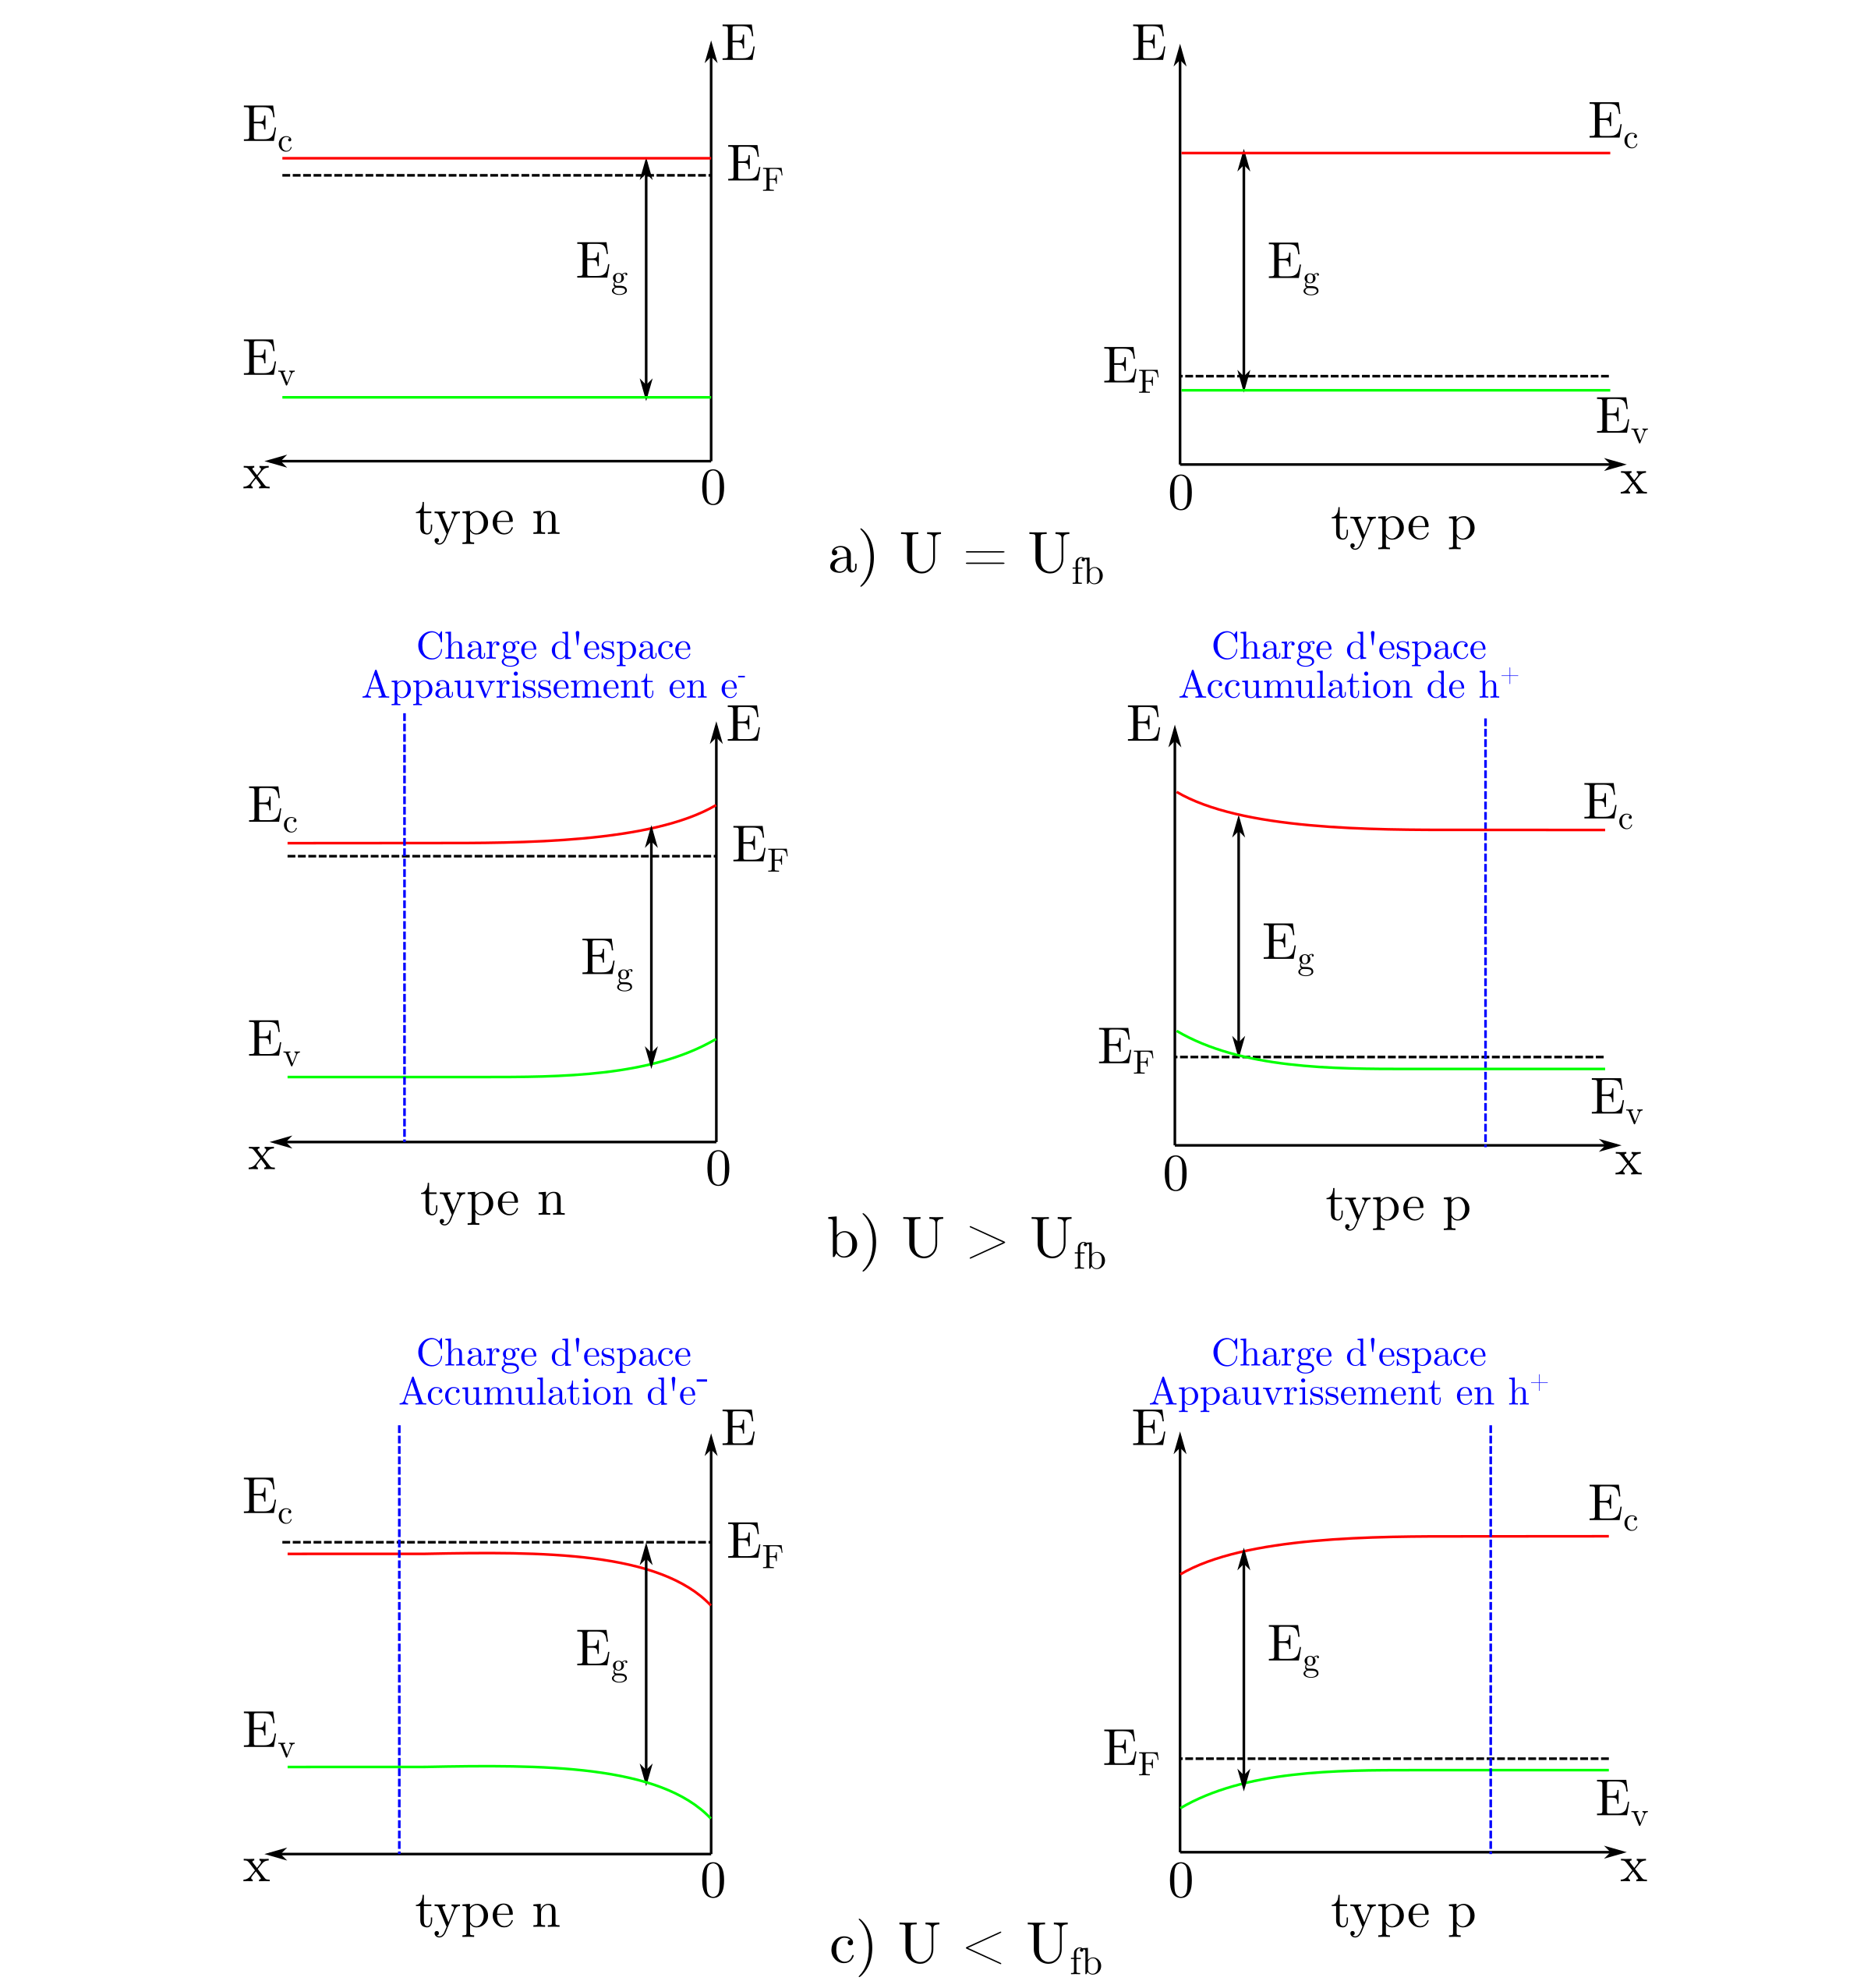
\includegraphics[width=0.85\textwidth]{Bending_Polarization.png}
        \caption[Représentation schématique des courbures de bandes pour des semiconducteurs de type \emph{n} et \emph{p}
        en contact avec un électrolyte en fonction de la polarisation appliquée: 
        a) U = $U_{fb}$,
        b) U > $U_{fb}$,
        c) U < $U_{fb}$.]
        {Représentation schématique des courbures de bandes pour des semiconducteurs de type \emph{n} et \emph{p}
            en contact avec un électrolyte en fonction de la polarisation appliquée (d'après \citet{Bard2002,
            Memming2008}): 
        a) U = $U_{fb}$, 
        b) U > $U_{fb}$, 
        c) U < $U_{fb}$.}
       \label{fig:bending_polarization}
    \end{figure}

    Sans illumination, des courants cathodiques (anodiques) vont être favorisés en situation d'accumulation d'électrons
    (trous) dans le cas d'un semiconducteur de type \emph{n} (\emph{p}). En effet, les porteurs de charge majoritaires
    d'un semiconducteur de type \emph{n} (\emph{p}) sont les électrons (trous). De manière réciproque, les courants
    anodiques (cathodiques) seront peu favorisés en situation d'appauvrissement dans le cas d'un semiconducteur de type
    \emph{n} (\emph{p}) puisque les trous (électrons) sont les porteurs de charge minoritaires. La jonction
    semiconducteur/électrolyte fonctionne comme une diode de Schottky.
             
    \subsubsection{Interface semiconducteur/électrolyte sous
    illumination}\label{subsec:semiconductor_electrolyte_contact_light}
     
    L'illumination d'une interface semiconducteur/électrolyte par des photons d'une énergie E ($h\nu$) supérieure
    au gap $\E_g$ génère des paires électron--trou dans le semiconducteur. En appliquant un potentiel adéquat,
    on peut séparer ces paires électron--trou de sorte que les 
    les porteurs de charge majoritaires soient évacués vers l'intérieur du semiconducteur alors que les
    porteurs de charge minoritaires rejoindront l'interface semiconducteur/électrolyte où ils pourront être transférer
    à une espèce redox présente dans
    l'électrolyte, générant un courant supplémentaire appelé \emph{photocourant}.

    La figure \ref{fig:photocurrent_generation} illustre de manière schématique le mécanisme de génération du photocourant.
    Pour un semiconducteur de type \emph{n} (\emph{p}), le photocourant est anodique (cathodique) puisque les électrons
    (trous) se dirigent vers le circuit externe alors que les trous (électrons) se dirigent vers l'interface externe. 
    Le photocourant devient donc significatif lorsque la jonction semiconducteur/électrolyte est en situation
    d'appauvrissement. Cela implique que le potentiel appliqué est supérieur (inférieur) au potentiel de bande plate
    dans le cas d'un semiconducteur de type \emph{n} (\emph{p}). 
    La figure \ref{subfig:ch1_Polarization_Curve-ntype} (\ref{subfig:ch1_Polarization_Curve-ptype}) illustre le
    photocourant anodique (cathodique) dans le cas d'un semiconducteur GaAs de type \emph{n} (\emph{p}).
    
    \begin{figure}[H]
        \centering
        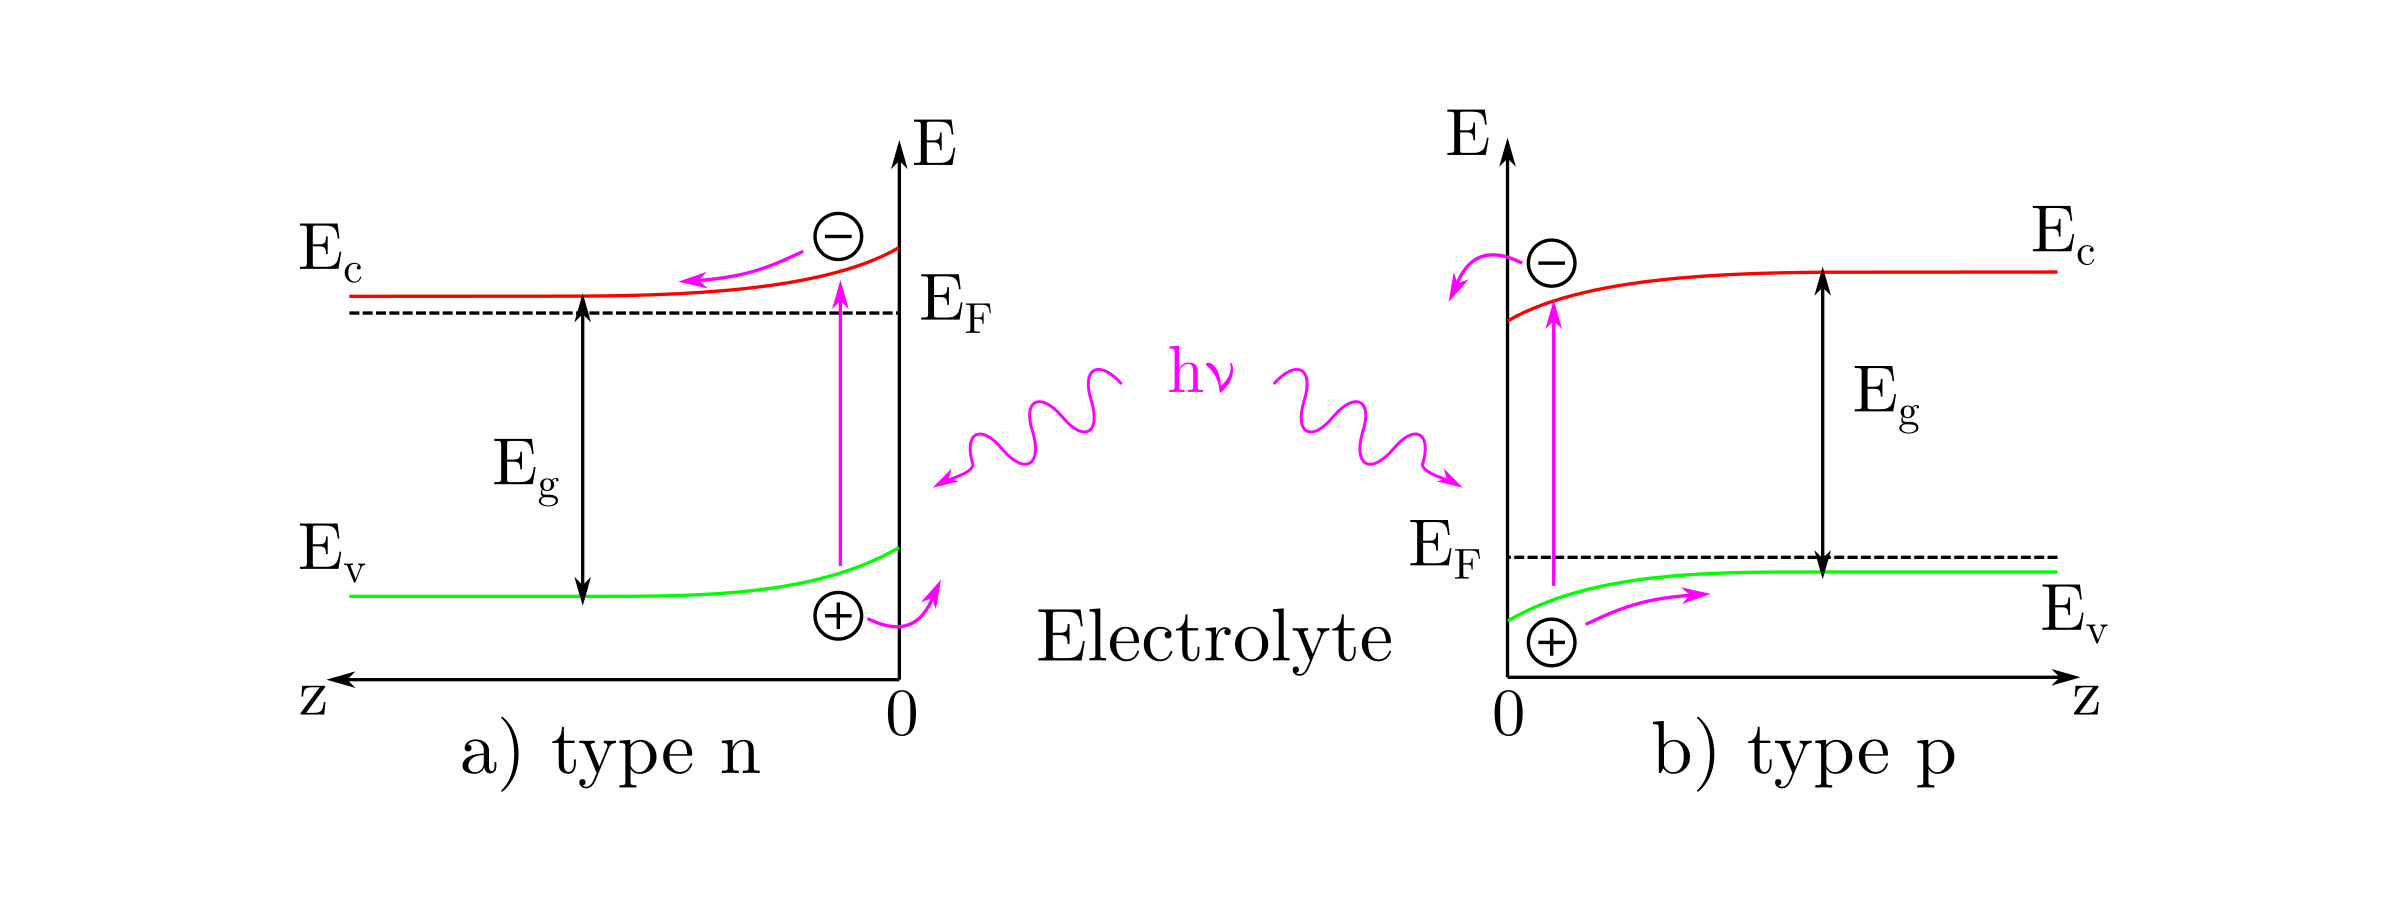
\includegraphics[width=0.85\textwidth]{Photocurrent_Generation.png}
        \caption[Représentation schématique du mécanisme de génération du photocourant.]
        {Représentation schématique du mécanisme de génération du photocourant (d'après \citet{Bard2002,
        Memming2008}).}
       \label{fig:photocurrent_generation}
    \end{figure}

    \begin{figure}[H]
        \centering
        \begin{subfigure}[b]{0.6\textwidth}
            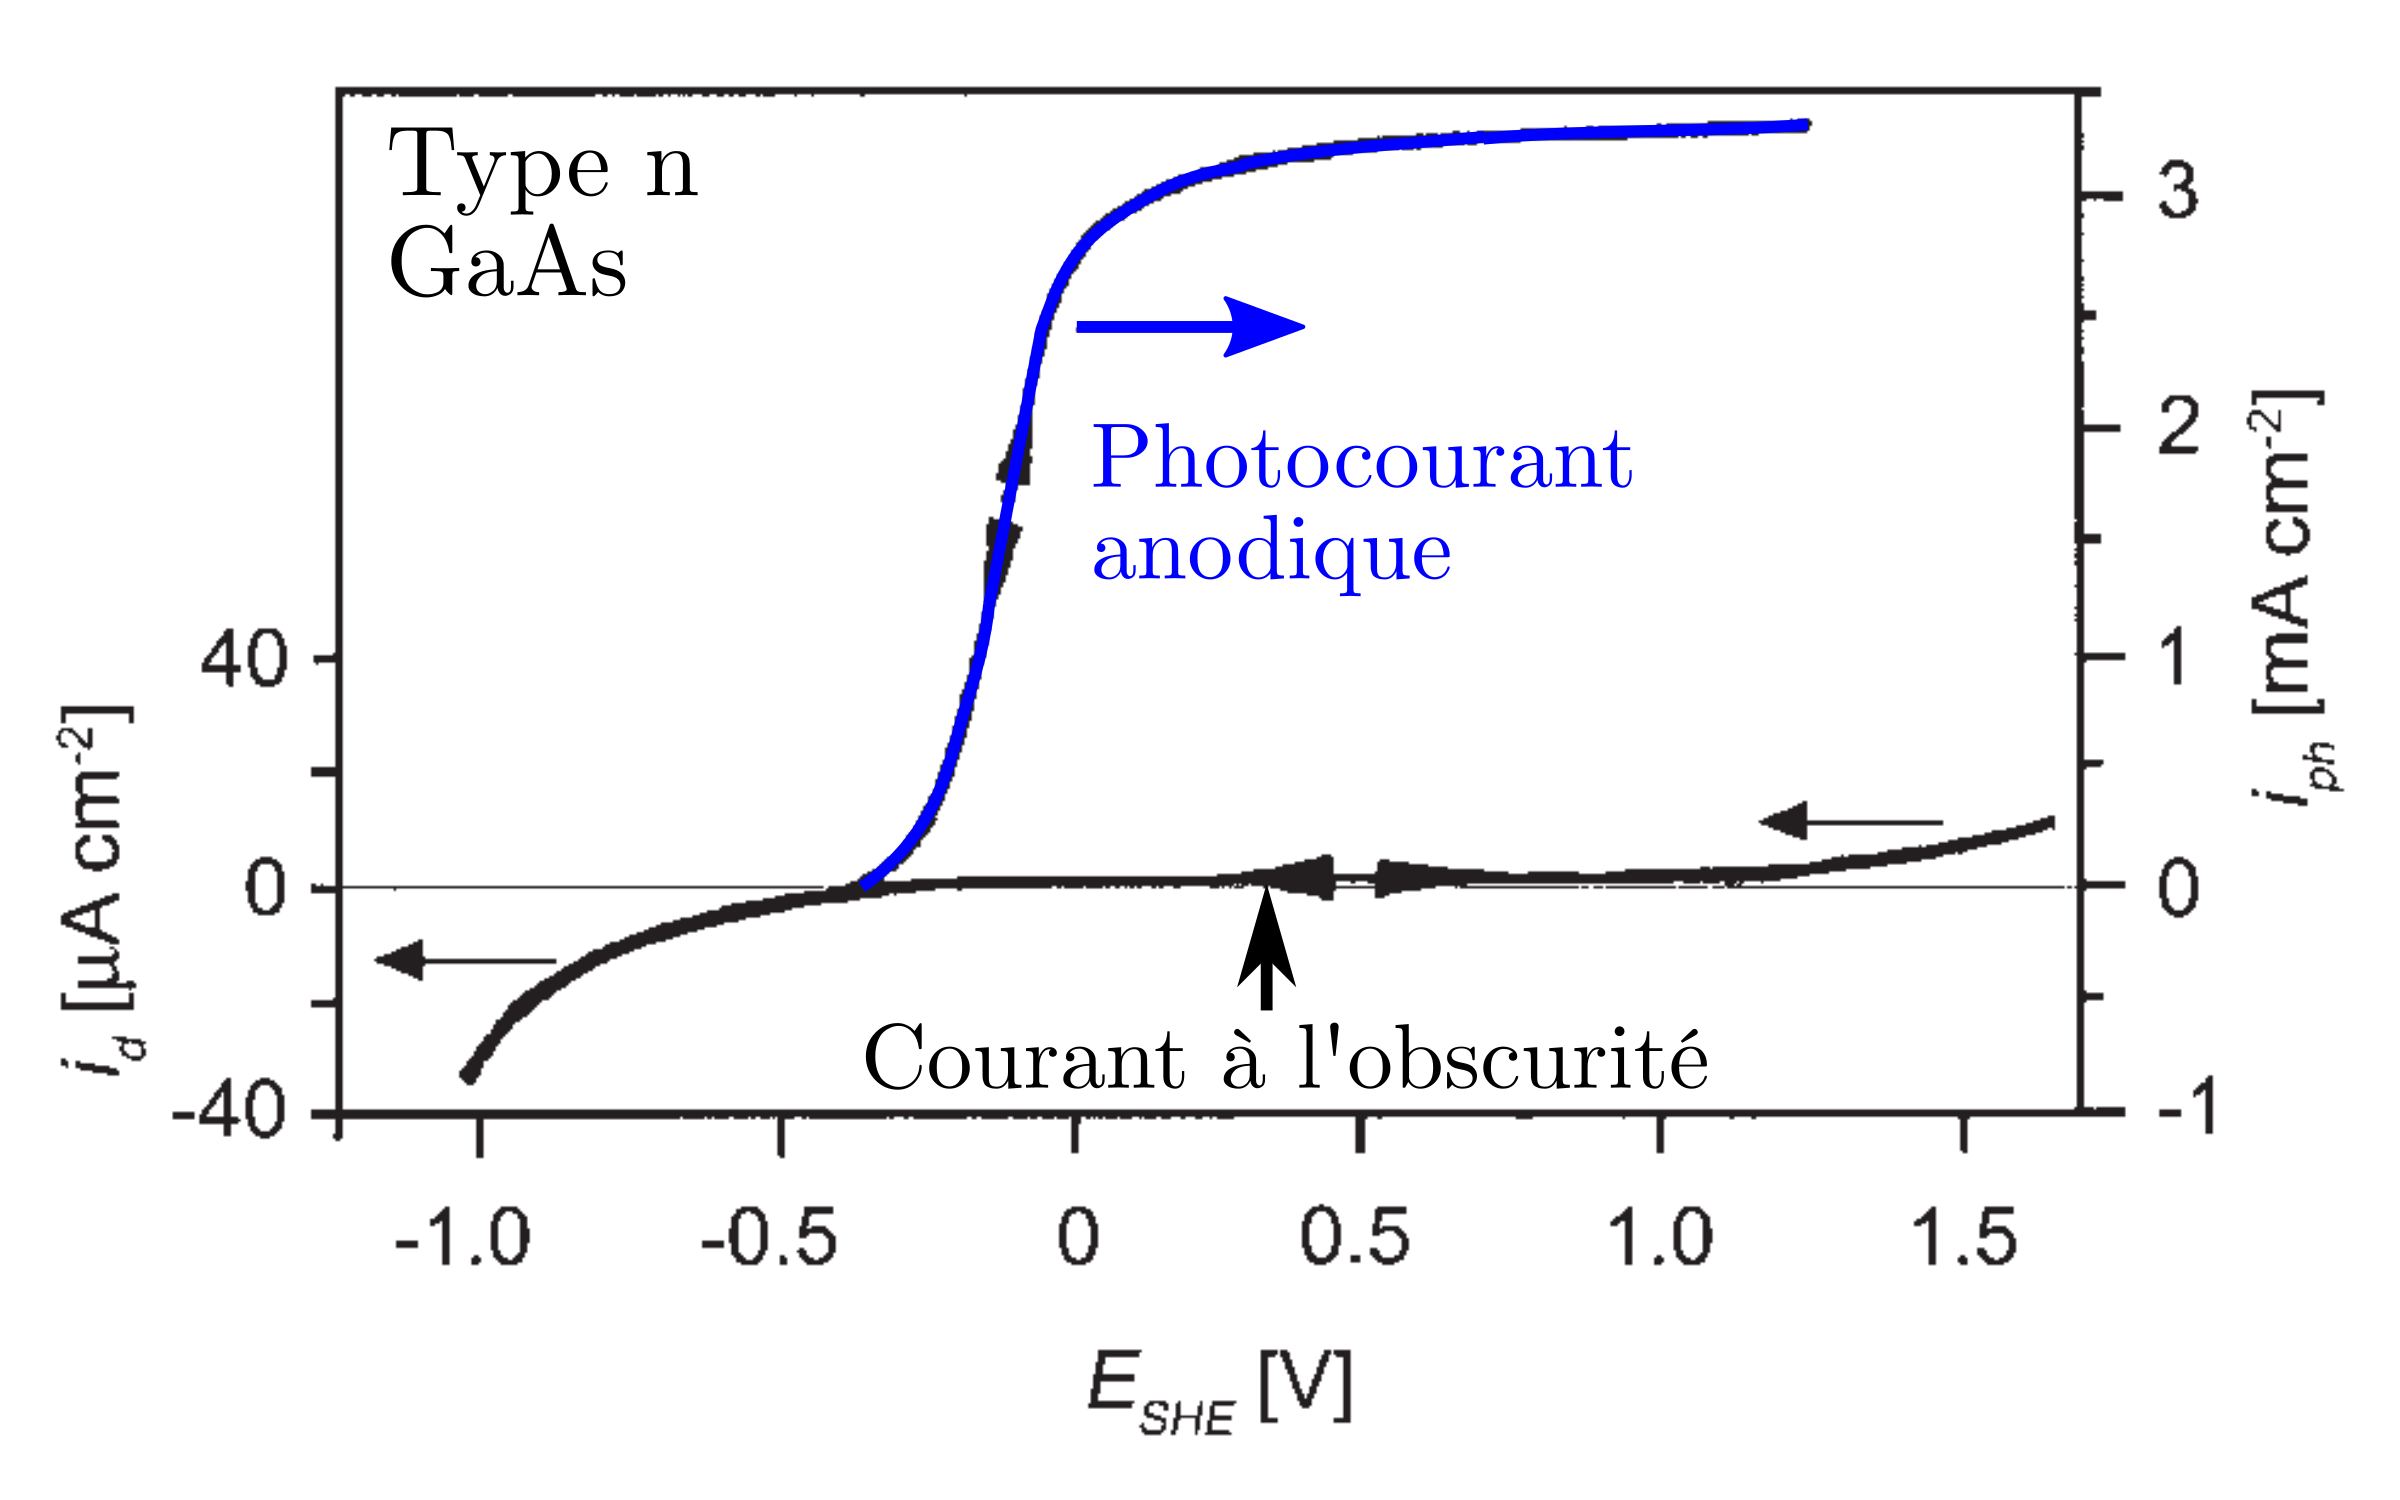
\includegraphics[width=\textwidth]{Iph_example_n_type.png}
            \caption{}
            \label{subfig:ch1_Polarization_Curve-ntype}
        \end{subfigure}

        \begin{subfigure}[b]{0.5\textwidth}
            \centering
            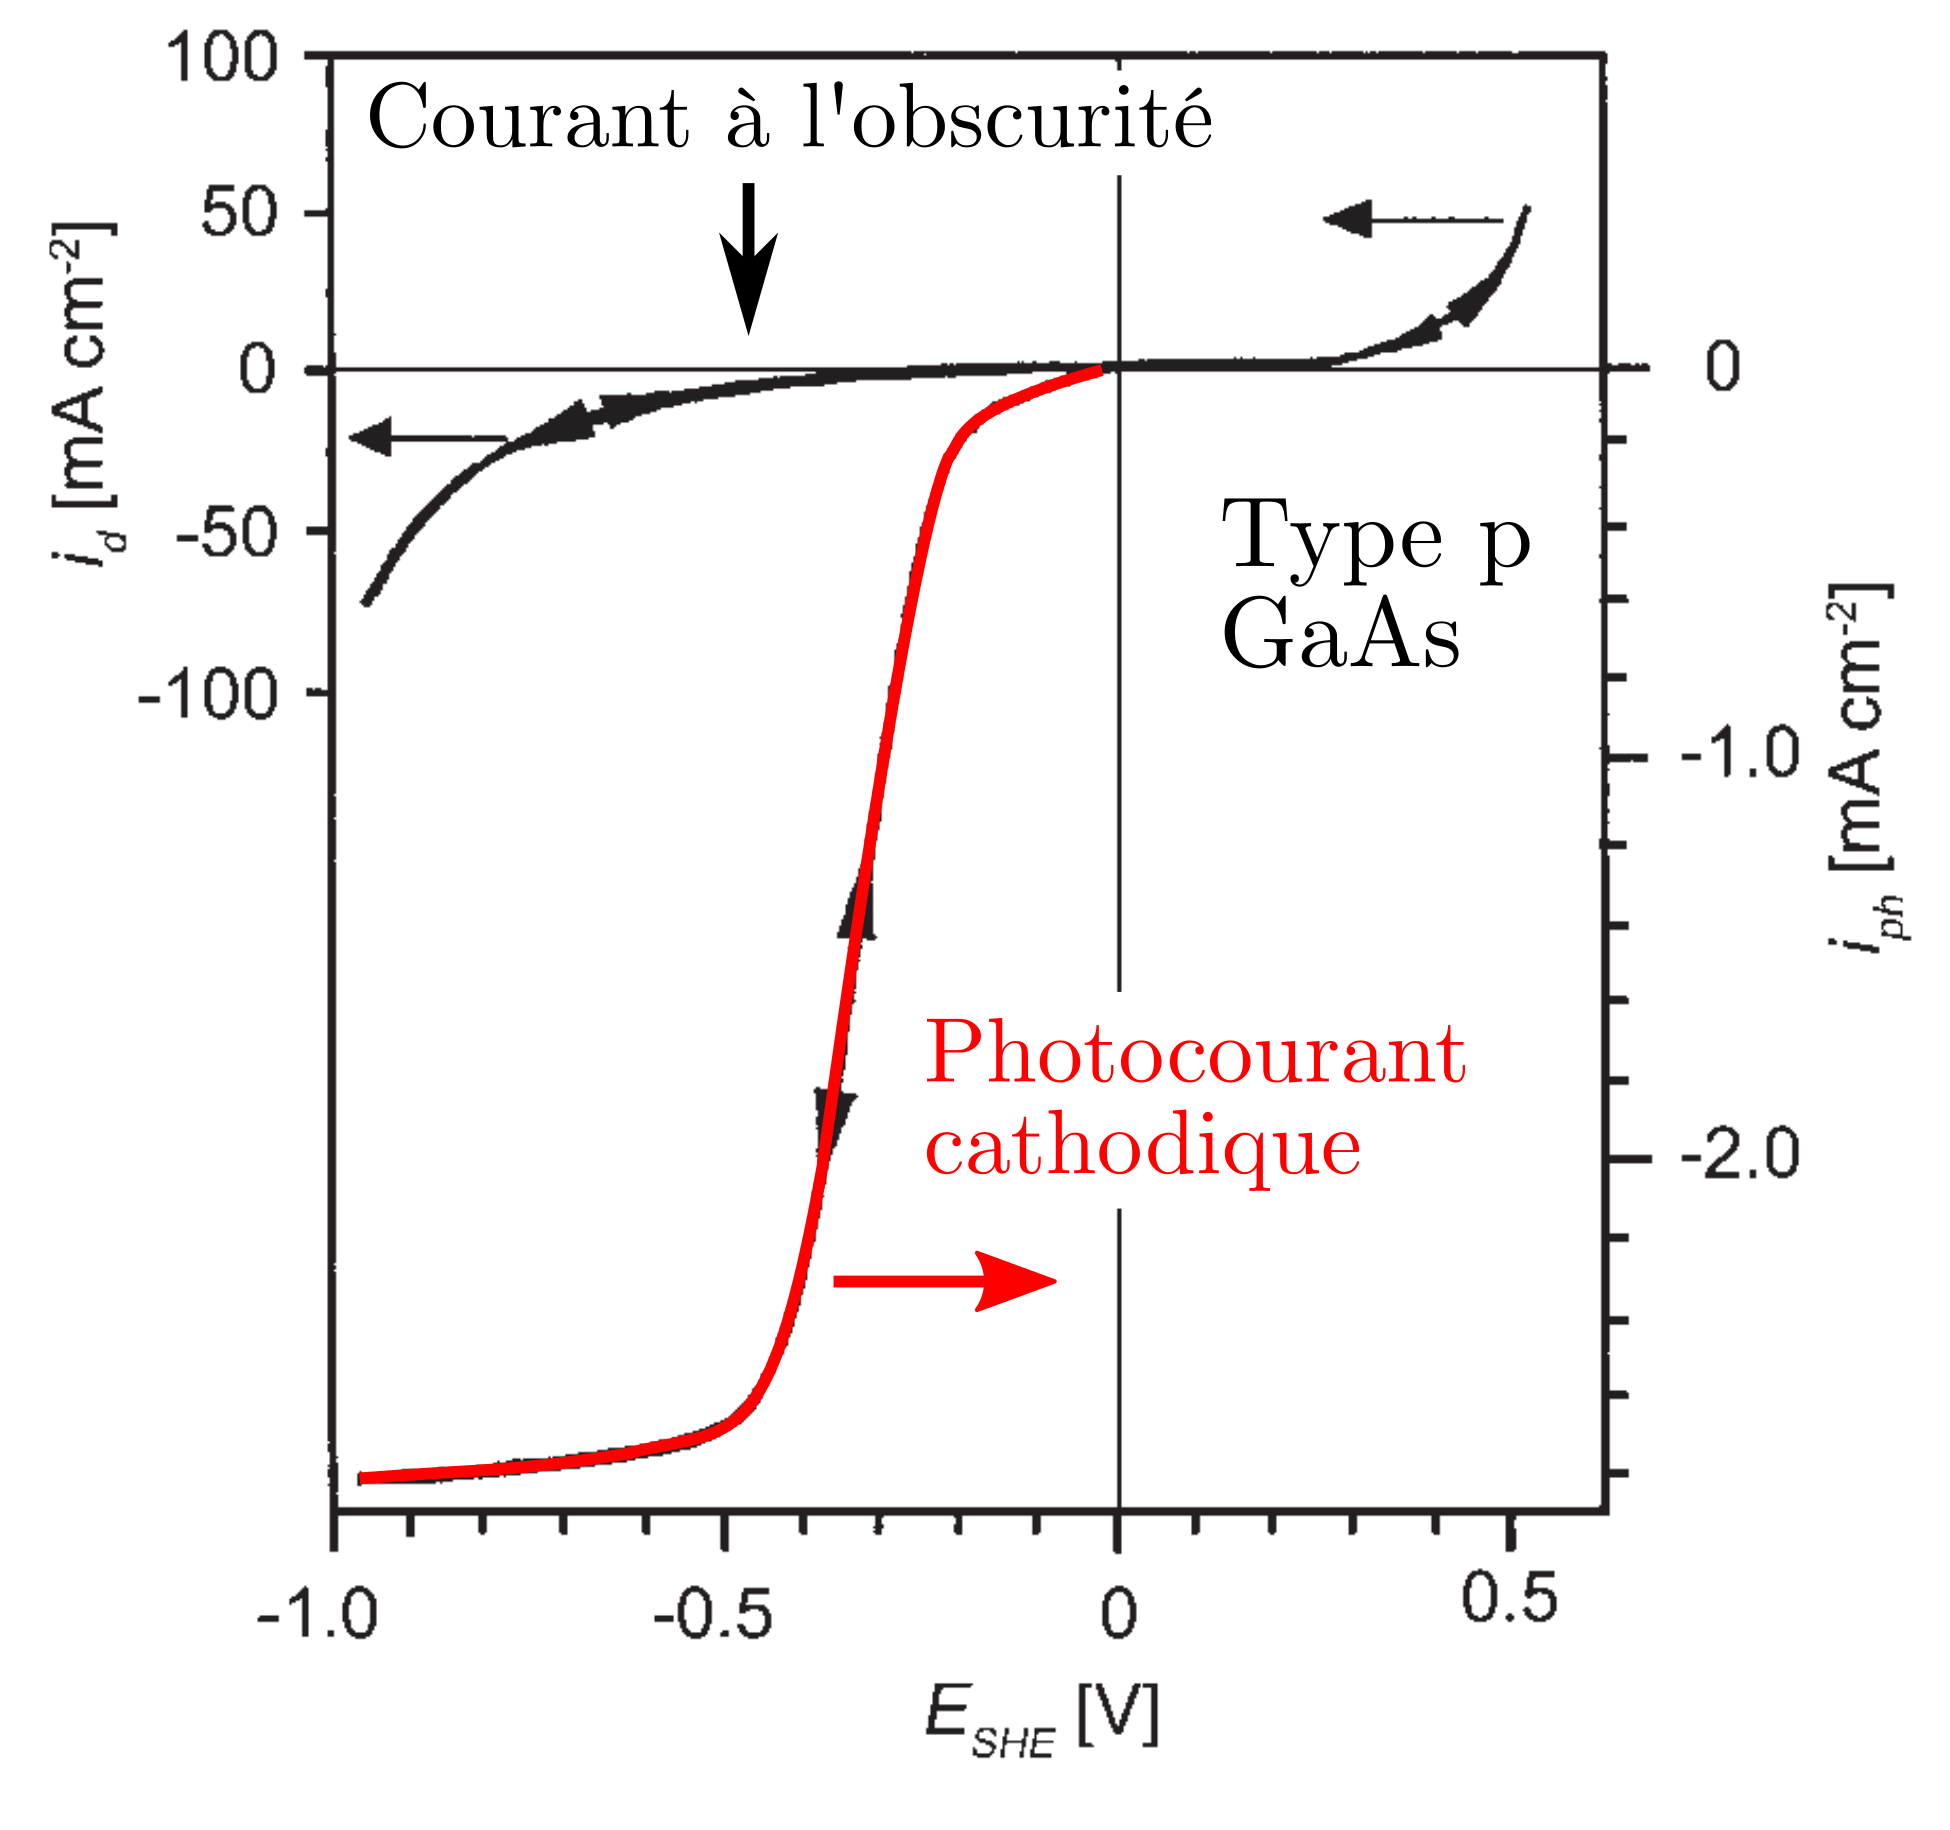
\includegraphics[width=\textwidth]{Iph_example_p_type.png}
            \caption{}
            \label{subfig:ch1_Polarization_Curve-ptype}
        \end{subfigure}
        \caption[Densité de photocourant $i_{ph}$ et densité de courant à l'obscurité $i_d$ en fonction du potentiel
            dans le cas du semiconducteur GaAs: 
            a) type \emph{n},
            b) type \emph{p}.]
        {Densité de photocourant $i_{ph}$ et densité de courant à l'obscurité $i_d$ en fonction du potentiel
            dans le cas du semiconducteur GaAs (d'après \citet{Plieth2008}): 
            a) type \emph{n},
            b) type \emph{p}.}
        \label{fig:ch1_photocurrent_examples}
    \end{figure}


    \citet{Gartner1959} et \citet{Butler1977} ont proposé un modèle, simple mais robuste, pour décrire le photocourant
    en faisant l'hypothèse que les paires électron--trou photogénérées dans la charge d'espace ne se recombinent pas. Le photocourant $\iph$
    est alors proportionnel au flux de photons incidents $\phi _0$. De plus, le photocourant dépend également du
    rapport relatif entre l'épaisseur de la charge d'espace $w_{\SC}$, la profondeur de pénétration des photons donnée
    par l'inverse du coefficient d'absorption $\alpha _{\SC}$ et de la longueur de diffusion moyenne des porteurs de
    charge minoritaires $L_{\cc}$. En d'autres termes, tous les
    photons absorbés dans une épaisseur égale à $w_{\SC} + L_{\cc}$ génèrent des paires électron--trou dont les porteurs de
    charge minoritaires sont transférés à l'électrolyte et par conséquent, participent au photocourant qui obéit donc à
    l'équation \ref{eq:iph_gartner_butler}. Lorsque $\alpha _{\SC} \cdot w_{\SC} \ll 1$ et $\alpha _{\SC} \cdot L_{\cc} \ll 1$, le photocourant peut être approximé par l'équation
    \ref{eq:iph_gartner_butler_simplified}.


    \begin{equation}
        I_{ph} = \phi _0 \left[ 1 - \frac{\exp (-\alpha _{\SC} \cdot w_{\SC})}{1+\alpha _{\SC} \cdot
        L_{\cc}} \right]
        \label{eq:iph_gartner_butler}
    \end{equation}

     \begin{equation}
        I_{ph} = \phi _0 \cdot \alpha _{\SC} \cdot w_{\SC}
        \label{eq:iph_gartner_butler_simplified}
    \end{equation}

    L'expression de l'épaisseur de la charge d'espace $w_{\SC}$, en situation d'appauvrissement, est donnée par
    l'équation \ref{eq:Space_charge_Schottky} dans le cadre de la théorie de Mott-Schottky. $N_{\cc}$ représente la
    concentration des porteurs de charge majoritaires, supposée égale au taux de dopage, $e$ correspond à la charge
    élémentaire de l'électron, U représente le potentiel appliqué à l'électrode, $U_{fb}$ représente le potentiel de
    bande plate, $\epsilon$ et $\epsilon _0$ représentent la permittivité relative du semiconducteur et la
    permittivité du vide, respectivement.
    
    \begin{equation}
        w_{\SC} = \sqrt{ \frac{2\epsilon \epsilon _0}{e N_{\cc}} (U-U_{fb}-\frac{kT}{e}) }
        \label{eq:Space_charge_Schottky}
    \end{equation}

    L'expression la plus utilisée du coefficient d'absorption $\alpha _{\SC}$ en fonction de l'énergie
    $h\nu$ des photons incidents est donnée par l'équation \ref{eq:absorption_coef}. La valeur de n dépend du type
    de transition bande--bande. Lorsque les transitions permises sont \emph{directes}, n vaut 0.5 alors que dans le cas des
    transitions \emph{indirectes}, n vaut 2.

    \begin{equation}
        \alpha _{\SC} = const \frac{(h\nu - \E_g)^n}{h\nu}
        \label{eq:absorption_coef}
    \end{equation}

    
    La dépendance en potentiel et en énergie du photocourant $\iph$ est donnée par l'équation
    \ref{eq:iph_substitute_W_alpha}. Cette
    dernière est obtenue en substituant l'épaisseur de la charge d'espace
    $w_{\SC}$ et le coefficient d'absorption $\alpha _{\SC}$ de l'équation \ref{eq:iph_gartner_butler_simplified} par
    les  équations \ref{eq:Space_charge_Schottky} et \ref{eq:absorption_coef}, respectivement.
             
     \begin{equation}
        I_{ph} = \phi _0 \cdot const \frac{(h\nu - \E_g)^n}{h\nu}
         \cdot \sqrt{ \frac{2\epsilon \epsilon _0}{e N_{\cc}} (U-U_{fb}-\frac{kT}{e}) }
        \label{eq:iph_substitute_W_alpha}
    \end{equation}

    A potentiel constant, la \emph{transformée linéaire} en énergie de l'équation
    \ref{eq:iph_substitute_W_alpha} est donnée par l'équation \ref{eq:iph_linear_transform}. A énergie constante, la \emph{transformée linéaire} en potentiel
    de l'équation \ref{eq:iph_substitute_W_alpha} est donnée par l'équation \ref{eq:iph_linear_transform_potential}.
    La transformée linéaire en énergie est utilisée pour déterminer des gaps (nous y reviendrons plus tard) alors que la
    transformée linéaire en potentiel est utilisée pour déterminer le type de semiconduction ainsi que les
    potentiels de bande plate.
    
    \begin{equation}
        \left[ \frac{I_{ph} \cdot h\nu}{\phi _0} \right] ^{1/n} = const \cdot (h\nu - \E_g)
        \label{eq:iph_linear_transform}
    \end{equation}

     \begin{equation}
        I_{ph}^2 = const \cdot (U-U_{fb}-\frac{kT}{e})
        \label{eq:iph_linear_transform_potential}
    \end{equation}

    
    \subsection[Exemples d'application de la photoélectrochimie]
    {Exemples d'application de la photoélectrochimie aux alliages de zirconium et aux alliages de
    nickel}\label{subsec:ch1_PEC_applications}

    \subsubsection{Identification des oxydes minoritaires}
     
    Les travaux de \citet{Benaboud2007} illustrent bien que la caractérisation photoélectrochimique se révèle être un outil
    performant pour mettre en évidence la présence d'oxydes
    mineurs dans la couche de zircone formée sur des échantillons de Zircaloy-4 par rapport à de la zircone formée sur du
    zirconium "pur". Les deux échantillons ont été oxydés en micro-thermobalance à \SI{470}{\degreeCelsius} avec une pression d'oxygène de
    \SI{150}{\milli\bar} pendant 1~h.
    
    Tout comme l'alliage Zircaloy-2, l'alliage Zircaloy-4 contient des éléments d'alliage (étain, fer, chrome) 
    se trouvant sous forme de précipités
    dans le métal. Lors de l'oxydation, ces éléments d'alliage se retrouvent dans la couche de zircone qui se forme à la
    surface et peuvent potentiellement être oxydés.
    Ces précipités oxydés sont des phases d'oxyde minoritaires dans la couche de zircone.
    En revanche la zircone qui se forme sur le zirconium "pur" ne devrait pas contenir de phases minoritaires. 
    En pratique, le zirconium "pur" contient des traces impuretés (fer et chrome) mais dont les concentrations sont bien
    plus faibles
    (environ dix fois moins de fer et environ cinq fois moins de chrome) que dans le cas de l'alliage Zircaloy-4.
    
    La figure \ref{subfig:benaboud_fig4} présente les spectres en énergie de photocourants mesurés sur l'alliage
    Zircaloy-4 et le zirconium "pur" où le fort photocourant observé à 5~eV, pour le Zircaloy-4 et le zirconium "pur",
    est une signature de l'oxyde majoritaire en l'occurrence la zircone monoclinique.
    Les photocourants mesurés sur les deux échantillons ne sont pas nuls aux basses énergies (<5~eV) mais leurs amplitudes 
    ne sont pas identiques, comme on peut l'observer en figure \ref{subfig:benaboud_fig5}.
    Ces photocourants mesurés à basse énergie sont des signatures des oxydes mineurs provenant des précipités oxydés.
    Malgré des concentrations en fer et chrome moins élevées dans l'échantillon de zirconium "pur", la caractérisation
    photoélectrochimique est suffisamment sensible pour détecter la présence de ces oxydes mineurs. 
   
    Les ruptures de pentes observées sur les spectres en énergie de photocourants permettent d'avoir une estimation des gaps des oxydes
    mineurs et de les identifier en s'appuyant sur les données de la littérature.
    Ainsi, l'auteur
    identifie de l'hématite $Fe_2O_3$, de la chromine $Cr_2O_3$ et une solution solide $(Fe_xCr_{1-x})_2O_3$.


    \begin{figure}[H]
        \centering
        \begin{subfigure}[b]{0.65\textwidth}
            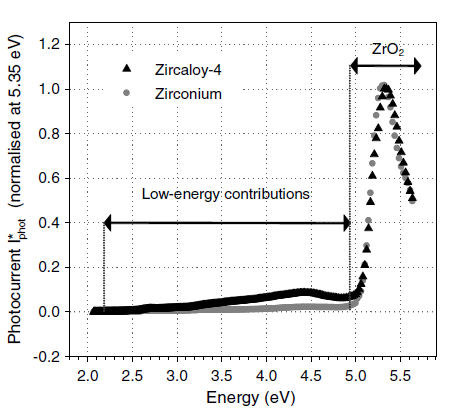
\includegraphics[width=\textwidth]{Benaboud2007-Fig4.png}
            \caption{}
            \label{subfig:benaboud_fig4}
        \end{subfigure}
        \begin{subfigure}[b]{0.65\textwidth}
            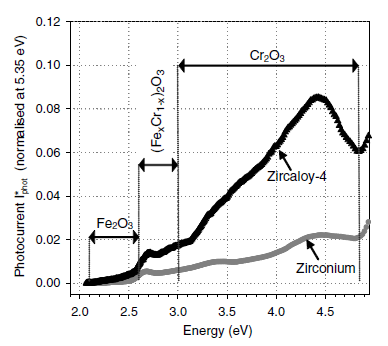
\includegraphics[width=\textwidth]{Benaboud2007-Fig5.png}
            \caption{}
            \label{subfig:benaboud_fig5}
        \end{subfigure}
        \caption[Spectres en énergie de photocourants mesurés sur des couches de zircone, sur un alliage
            Zircaloy-4 et sur 
            zirconium pur, formées à \SI{470}{\degreeCelsius} dans une atmosphère d'oxygène pendant 1~h:
            a) spectre complet de 2 à 5~eV, 
            b) zoom sur les contributions des oxydes mineurs.]
        {Spectres en énergie de photocourants mesurés sur des couches de zircone, sur un alliage Zircaloy-4 et sur 
            zirconium pur, formées à \SI{470}{\degreeCelsius} dans une atmosphère d'oxygène pendant 1~h \citep{Benaboud2007}:
            a) spectre complet de 2 à 5~eV, 
            b) zoom sur les contributions des oxydes mineurs.}
        \label{fig:benaboud_application}
    \end{figure}

    \subsubsection{Identification du type de semiconduction}

    Les travaux de \citet{Loucif2013} illustrent le changement de type de semiconduction des couches d'oxyde formées 
    sur des alliages de nickel oxydés en
    milieu primaire REP simulé pendant 500~h en fonction de la pression d'hydrogène (6.5 et \SI{0.05}{\bar}).
    La figure \ref{fig:loucif_application} présente les photocaractéristiques en potentiel mesurées pour différentes
    énergies dont les photocourants ont été normalisés à 1 à leur valeur maximale.
    
    A forte pression partielle d'hydrogène, la photocourant normalisé de la figure
    \ref{subfig:loucif_fig3_18} présente une forme en "V" suggérant un comportement isolant de la couche d'oxyde.
    En revanche, lorsque la pression partielle d'hydrogène est très faible, le photocourant normalisé de la figure \ref{subfig:loucif_fig3_19}
    augmente fortement lorsque le potentiel appliqué est de plus en plus anodique
    indiquant que la couche d'oxyde présente une semiconduction de type \emph{n}.
    
     \begin{figure}[H]
        \centering
        \begin{subfigure}[b]{0.48\textwidth}
            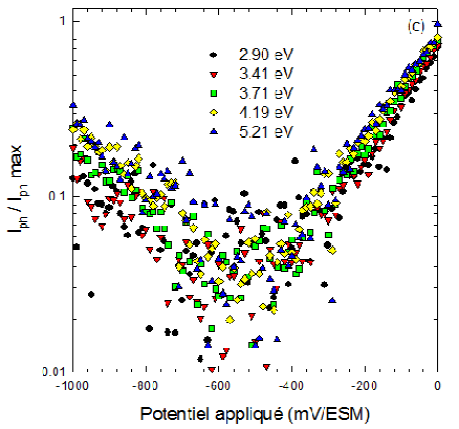
\includegraphics[width=\textwidth]{Loucif2012-Fig3-18.png}
            \caption{}
            \label{subfig:loucif_fig3_18}
        \end{subfigure}
        \begin{subfigure}[b]{0.48\textwidth}
            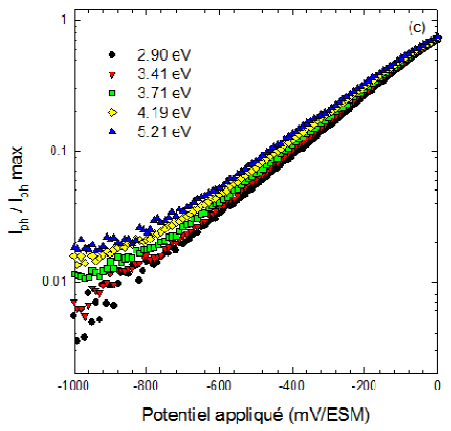
\includegraphics[width=\textwidth]{Loucif2012-Fig3-19.png}
            \caption{}
            \label{subfig:loucif_fig3_19}
        \end{subfigure}
        \caption[Photocaractéristique en potentiel de l'alliage 600 poli diamant et oxydé en milieu primaire REP simulé pendant
        500~h:
        a) $P_{H_2} = \SI{6.5}{\bar}$,
        b) $P_{H_2} = \SI{0.05}{\bar}$.]
        {Photocaractéristique en potentiel de l'alliage 600 poli diamant et oxydé en milieu primaire REP simulé pendant
            500~h \citep{Loucif2013}: 
        a) $P_{H_2} = \SI{6.5}{\bar}$,
        b) $P_{H_2} = \SI{0.05}{\bar}$.}
        \label{fig:loucif_application}
    \end{figure}

    Comme la majorité des caractérisations photoélectrochimiques, les deux exemples cités ci-dessus sont des
    caractérisations réalisées à température ambiante dans des cellules électrochimiques en verre.
    Réaliser des caractérisations photoélectrochimiques à haute température nécessite l'utilisation de cellules
    électrochimiques métalliques possédant un hublot pouvant laisser passer la lumière.
    \citet{Bojinov2002} ont montré la faisabilité à haute température sur des couches d'oxyde formées sur du
    fer pur. La figure \ref{subfig:Bojinov_HT_cell} illustre la cellule conçue pour travailler à
    haute température qui a permis d'obtenir des photocaractéristiques en énergie de la figure
    \ref{subfig:Bojinov_PEC_result}. Toutefois, la température a été limitée à \SI{200}{\degreeCelsius} et l'interval
    de travail en énergie a été limitée entre 1.8 et \SI{4}{\electronvolt}. A notre connaissance, cette étude est la
    seule dans le domaine de la photoélectrochimie à haute température.

	\begin{figure}[H] 
 		\centering 
            \begin{subfigure}[b]{0.55\textwidth}
                \includegraphics[width=\textwidth]{Bojinov_2002_Fig5b-redraw.png} 
                \caption{}
                \label{subfig:Bojinov_HT_cell}
            \end{subfigure}
            \quad
            \begin{subfigure}[b]{0.55\textwidth} 
                \includegraphics[width=\textwidth]{Bojinov_2002_Fig1.png} 
                \caption{}
                \label{subfig:Bojinov_PEC_result} 
           \end{subfigure}
       \caption[a) Spectres en énergie de photocourants à différentes températures mesurés sur des oxydes de fer
           (\SI{<200}{\degreeCelsius}, \SI{100}{\bar}),
                b) aperçu de la cellule de caractérisation photoélectrochimique.]
       {a) Spectres en énergie de photocourants à différentes températures mesurés sur des oxydes de fer
           (\SI{<200}{\degreeCelsius}, \SI{100}{\bar}),
       b) aperçu de la cellule de caractérisation photoélectrochimique \citep{Bojinov2002}.}
      \label{fig:HT_PEC_bojinov}
 	\end{figure}

%%%%%%%%%%%%%%%%%%%%%%%%%%%%%%%%%%%%%%%%%%%%%%%%%%%%%%%%%%%%%%%%%%%%%%%%%%%%%%%%%%%%%
%%%%%%%%%%%%%%%%%%%%%%%%%%%%%%%%%%%%%%%%%%%%%%%%%%%%%%%%%%%%%%%%%%%%%%%%%%%%%%%%%%%%%
\section{Conclusions}\label{sec:impacting_parameters}

    L'état de l'art exposé dans ce chapitre suggère que le phénomène de Shadow Corrosion résulte très
    probablement de la combinaison de quatre facteurs 
    liés au fonctionnement des REB: \emph{irradiation}, \emph{chimie de l’eau}, \emph{nature des matériaux} et la
    \emph{couplage galvanique} avec d’autres matériaux comme nous tentons de le schématiser en
    figure \ref{fig:impacting_parameters} où les principaux facteurs sont symbolisés par des cercles et les paramètres
    d'intérêt pour l'étude expérimentale sont symbolisés par des rectangles. 

    \begin{figure}[H] 
 		\centering 
 		\includegraphics[width=0.95\textwidth]{Impacting_Parameters-3.png} 
 		\caption{Principaux facteurs d'influence de la Shadow Corrosion et les paramètres d'intérêt pour son étude
        expérimentale.} 
 		\label{fig:impacting_parameters} 
 	\end{figure}

    Comme vu plus haut, l’irradiation que subissent les matériaux englobe des rayonnements électromagnétiques allant 
    des UV aux
    rayonnements $\gamma$ ainsi que le rayonnement neutronique. Ces rayonnements peuvent impacter le transport ionique
    ainsi que le transport électronique dans les oxydes formés sur les gaines de confinement et les grilles de maintien. 
    La principale conséquence de l'irradiation est selon nous la perturbation de l'équilibre qui s'établit entre le transport
    ionique et le transport électronique afin d'assurer l'électroneutralité dans la couche de zircone.
    %Toutefois, il
    %semble y avoir peu de preuves avérées sur le lien direct entre l’accélération de la cinétique de corrosion et 
    %l’augmentation des coefficients de diffusion de l’oxygène dans la couche de zircone.

    Etudier l'impact du rayonnement neutronique et du rayonnement $\gamma$ nécessite des moyens expérimentaux
    conséquents. En revanche, l'illumination avec de la lumière UV semble être un moyen plus accessible 
    permettant de tenter de simuler
    une partie de l'effet de l'irradiation, à condition de disposer d'un flux non négligeable de photons y compris
    pour ceux ayant une énergie
    supérieure au gap de la zircone monoclinique soit \SI{5}{\electronvolt}.

    Nous avons également vu que la radiolyse de l’eau crée des espèces radicalaires ayant un pouvoir oxydant élevé. La
    recombinaison de ces espèces produit principalement du peroxyde d’hydrogène, qui augmente le
    pouvoir oxydant de l'électrolyte et peut potentiellement entraîner une dissolution partielle de la zircone. 
    Des injections en continu de péroxyde d'hydrogène dans l'électrolyte pourront permettre de simuler l'effet chimique
    de la radiolyse. 
    
    Les éléments fer, nickel et chrome, provenant de la dissolution des phases intermétalliques 
    peuvent doper la couche de zircone et ainsi modifier le comportement électrochimique global des alliages Zy2.
    De plus, ces mêmes éléments peuvent être présents dans l'électrolyte et sont susceptibles de modifier le
    comportement électrochimique global du Zy2 et de l'Inconel 718.
    Même si le lien entre la présence de cations dans
    l'électrolyte et l'accélération de la corrosion des alliages de zirconium n'est pas clairement établi, il sera
    possible de modifier la chimie de l'électrolyte pour examiner l'influence de ces cations sur le comportement
    électrochimique des alliages.
   
    Les méthodes électrochimiques classiques semblent bien être adaptée à l'étude des comportements
    électrochimiques des matériaux dans le cadre du mécanisme de couplage galvanique proposé par \citet{Lysell2004} et
    également modélisé par \citet{Buttin2011}.
    Nous nous axerons sur trois techniques: suivi du potentiels électrochimiques, suivi de courants de
    couplages et tracés de courbes de polarisation. Ces techniques seront présentées dans le
    chapitre 2.

    La technique de caractérisation photoélectrochimique (PEC) est moins communément utilisée mais est performante
    pour suivre les modifications subies par la couche d'oxydation en fonction des conditions expérimentales. 
    Afin de pouvoir réaliser des photocaractéristiques en énergie et/ou en potentiel à la température d'un réacteur à
    eau bouillante, soit
    \SI{280}{\degreeCelsius}, il a été nécessaire de développer une cellule électrochimique spécifique.
    Les étapes de conception, développement et de validation de l'installation développée seront décrites au chapitre
    \ref{chap:design}.
    Le chapitre 4 sera axé sur la présentations et la discussion des résultats de notre étude.

    % \ref{chap:ch4_results}
    \singlespacing
\printbibliography[heading=subbibintoc]
    \onehalfspacing
\end{refsection}
